\ifnum \aluno=1
\renewcommand\chapterillustration{abertura-funcoes}
\else
\renewcommand\chapterillustration{abertura-funcoes-professor}
\fi
\renewcommand\chapterwhat{Funções e suas diferentes representações (numérica, algébrica e gráfica); domínio, contradomínio e imagem; aplicações em situações envolvendo a análise, interpretação e resolução de problemas em contextos diversos.}
\renewcommand\chapterbecause{Funções são objetos matemáticos que nos permitem compreender como a variação de uma grandeza influencia na variação de outra. Por isso elas são ferramentas essencias para a compreensão, análise e tomada de decisão em diversas situações do nosso dia a dia.
O estudo de funções nos permite, por exemplo, relacionar a área de um polígono com o comprimento de seus lados, a distância percorrida por um objeto com o intervalo de tempo gasto no percurso e o valor da conta de energia elétrica com o consumo de energia.
De um modo mais geral, funções são úteis para o estudo do crescimento populacional, disseminação de doenças, lançamento de foguetes e satélites, interpretação de exames médicos, etc.}
\chapter{Introdução às Funções}

\mbox{}\thispagestyle{empty}\clearpage

\thispagestyle{empty}
\def\funcoeschap{}

\begin{center}
Projeto: LIVRO ABERTO DE MATEMÁTICA

\noindent \begin{tabular}{lcccr}

\includegraphics[scale=.15]{impa}& \quad\quad& 
\includegraphics[width=3cm]{logo} & \quad\quad& 
\includegraphics[scale=.24]{obmep} 
\end{tabular}
\end{center}

\vspace*{.3cm}

Cadastre-se como colaborador no site do projeto: \url{umlivroaberto.org}

Versão digital do capítulo:

\url{https://www.umlivroaberto.org/BookCloud/Volume_1/master/view/AF106.html}


\begin{tabular}{p{.15\textwidth}p{.7\textwidth}}
Título: & Introdução às Funções\\
\\
Ano/ Versão: & 2020 / versão 1.0 de \today\\
\\
Editora & Instituto Nacional de Matem\'atica Pura e Aplicada (IMPA-OS)\\
\\
Realização:& Olimp\'iada Brasileira de Matem\'atica das Escolas P\'ublicas (OBMEP)\\
\\
Produção:& Associação Livro Aberto\\
\\
Coordenação:& Fabio Simas, \\
			& Augusto Teixeira (livroaberto@impa.br)\\
\\
  Autores: & Gladson Antunes (UNIRIO),\\
        & Michel Cambrainha (UNIRIO),\\
           
\\
Revisoras: &  Cydara Ripoll  \\
                &  Letícia Rangel \\
\\
Design: & Andreza Moreira (Tangentes Design) \\
\\
  Ilustrações: & --- \\ 
\\
Gráficos: & Beatriz Cabral e Tarso Caldas (Licenciandos da UNIRIO)\\
\\
  Capa: & Foto de Engin Akyurt, no Pexels \\
  		& https://www.pexels.com/pt-br/foto/animacao-ao-ar-livre-ativo-borrao-1435537/
\end{tabular}
\vspace{.5cm}


\begin{figure}[b]
\begin{minipage}[l]{5cm}
\centering

{\large Licença:}

  
\includegraphics[width=3.5cm]{cc-by-sa1.png}
\end{minipage}\hfill
\begin{minipage}[c]{5cm}
\centering
{\large Desenvolvido por}


\includegraphics[width=2.5cm]{logo-associacao.jpg}
\end{minipage}
\begin{minipage}[r]{5cm}
\centering

{\large Patrocínio:}
  \vspace{1em}
  
\includegraphics[width=3.5cm]{itau}
\end{minipage}
\end{figure}

\mainmatter

\begin{apresentacao}{Introdução}

Muitas situações e decisões do dia a dia dependem do reconhecimento de uma relação entre duas grandezas e da análise de como a variação de uma delas influencia na variação da outra (Por exemplo, a distância percorrida e o tempo, a área de um polígono e o comprimento de seus lados, a absorção de um medicamento pelo organismo humano e o tempo desde a sua ingestão, valor da conta de energia elétrica e consumo, quantidade de vereadores e a população etc). O tema \textit{funções} trata da relação entre grandezas, sendo uma ferramenta matemática importante para descrever, analisar e tomar decisões em diversas situações. Além disso, na Matemática como ciência, função é considerado um conceito fundamental e elementar para que outros conceitos e resultados da própria Matemática sejam estabelecidos.

\subsection{Objetivos do capítulo}:

\begin{habilities}{EM11MT06}

Compreender função como uma relação de dependência entre duas variáveis, as ideias de domínio, contradomínio e imagem, e suas representações algébricas e gráficas e utilizá- las para analisar, interpretar e resolver problemas em contextos diversos, inclusive fenômenos naturais, sociais e de outras áreas.

Espera-se também que o estudante compreenda função como uma relação unívoca entre duas variáveis.
\end{habilities}

Destaca-se que, segundo a Base Nacional Comum Curricular (BNCC), no nono ano do Ensino Fundamental, é esperado que o estudante tenha alcançado a habilidade: \textbf{(EF09MA06)} Compreender as funções como relações de dependência unívoca entre duas variáveis e suas representações numérica, algébrica e gráfica e utilizar esse conceito para analisar situações que envolvam relações funcionais entre duas variáveis. O foco nessa habilidade é retomado neste capítulo com os propósitos de revisão e de aprofundamento, visando aos objetivos indicados acima.

O capítulo tem início com a seção \textit{Explorando}, que propõe três atividades que envolvem aspectos fundamentais da definição de função e algumas formas de representação. Serão tratadas a relação de dependência, a existência de correspondência e a univocidade. Essas atividades têm também o objetivo de resgatar conceitos já tratados no Ensino Fundamental, tais como reconhecimento de padrões, leitura e interpretação de gráficos. Na primeiro \textit{Organizando as Ideias} desse capítulo, o conceito de função é formalizado e, em seguida, na seção \textit{Praticando}, é explorado a partir de atividades variadas.  A primeira parte do capítulo termina com uma seção de \textit{Aprofundando}, na qual são propostos problemas e situações em que os conceitos e as ideias já tratados são explorados em contextos mais desafiadores. Na segunda parte, em uma nova seção \textit{Explorando}, a representação gráfica de função é abordada. Algumas das atividades já apresentadas anteriormente são revisitadas, e são propostas outras nas quais discutem-se vantagens e desvantagens da representação gráfica quando comparada com tabelas, a localização de pontos no plano cartesiano a partir de situações reais e a representação gráfica para pares ordenados com coordenada não numérica. Em seguida, em um segundo \textit{Organizando as ideias}, o conceito de representação gráfica é formalizado, para logo após ser explorado em outra seção \textit{Praticando}. O capítulo encerra com um \textit{Aprofundamento}, no qual são propostas duas atividades que relacionam os conceitos apreendidos com problemas de Modelagem Matemática, e uma proposta de Projeto Aplicado, em que os estudantes são estimulados a construírem uma caixa de volume máximo.

\paragraph{Algumas observações}

\begin{itemize}
\item {} 
O conceito de função é apresentado e explorado de maneira contextualizada e geral, isto é, não restrito apenas a conjuntos numéricos. Assim, busca-se ressaltar que a importância desse conceito transcende a Matemática alcançando outras áreas do conhecimento.

\item {} 
Reconhecer a dependência, observando como a variação de uma ou mais grandezas afeta        a variação de outras, é um objetivo. A partir dessse reconhecimento, sempre que possível, busca-se, usando linguagem matemática ou não, estabelecer uma maneira de descrever a relação observada.

\item {} 
A univocidade como condição para que uma relação entre grandezas ou variáveis seja identificada como função é destacada desde as atividades iniciais.

\item {} 
As conversões entre representações algébrica e gráfica são de vital importância para a compreensão do conceito de função, amparando a análise e a interpretação das relações existentes entre as variáveis envolvidas.

\item {} 
Incentive e conduza seus estudantes a expressarem seus raciocínios de maneira precisa, mesmo que seja apenas usando palavras, tanto de forma verbal como escrita.

\item {} 
Ao criar suas próprias atividades, sugerimos que sejam evitadas as que envolvem cálculos algébricos exaustivos.

\item {} 
Nas atividades extras que você venha a apresentar para seus estudantes, é importante estar atento para não reforçar a crença bastante comum de que relações entre grandezas são sempre proporcionais.

\end{itemize}

\paragraph{O que dizem as pesquisas sobre o tema?}

A noção de função é considerada uma das mais importantes da matemática. Segundo \cite{Ponte1992}, assim como o ponto, a reta e o plano são conceitos básicos da Geometria Euclidiana, o  conceito de função tem um papel fundamental na Análise Matemática. Documentos oficiais como os Parâmetros Curriculares Nacionais do Ensino Médio (PCNEM) e a (segunda versão da) Base Nacional Comum Curricular (BNCC)  evidenciam a preocupação com tal conteúdo no Ensino Médio, trazendo inclusive sugestões no que diz respeito a sua abordagem.
\begin{quote}

Nessa etapa de escolaridade, merece especial destaque o estudo das funções por seu papel como modelo matemático para analisar e interpretar relações de dependência entre variáveis de duas grandezas em fenômenos do mundo natural ou social, incluindo os trabalhados em componentes de outras áreas de conhecimento \citep[p.576]{BNCC2016}.

O estudo das funções permite ao aluno adquirir a linguagem algébrica como a linguagem das ciências, necessária para expressar a relação entre grandezas e modelar situações-problema, construindo modelos descritivos de fenômenos e permitindo várias conexões dentro e fora da própria matemática. (PCNEM-2006, p.121)
\end{quote}

São muitos os relatos sobre as  diversas dificuldades que os estudantes apresentam no processo de aprendizagem da noção de função. \cite{Sierpinska1992} chama atenção para alguns dos problemas mais comuns:  fazer a ligação entre as diferentes representações (fórmulas, gráficos, diagramas, descrição por palavras); interpretar gráficos e manipular algebricamente, entre outros.

Neste ponto do desenvolvimento do seu aprendizado é muito comum o estudante fazer confusão entre os diferentes papéis que as variáveis (letras) representam nas expressões algébricas. Para \cite{Ursini2001}, as distintas interpretações possíveis para a simbologia algébrica constituem aspectos que geram dificuldades adicionais a muitos estudantes.

Segundo \cite{Eisenberg1992}, os estudantes têm uma forte tendência para pensar em funções algebricamente, em vez de visualmente, mesmo que a visualização possa ser extremamente útil. Segundo esse autor, os estudantes resistem às representações visuais porque o processamento visual requer habilidades de nível mais elevado do que o processamento analítico.

\begin{figure}[H]
\centering

\noindent\includegraphics[width=.75\linewidth]{{caixa_3}.png}
\end{figure}

\cite{Jones2006} chama atenção para três níveis de abstração nos quais é possível situar o entendimento do conceito de função:  como \textit{ação}, como \textit{processo} e como \textit{objeto}. O nível ação é aquele em que são conhecidas todas as ações que devem ser tomadas para converter a variável independente \(x\) na sua imagem, por exemplo: tome \(x\), primeiro eleve ao quadrado e então subtraia do seu dobro. Nesse nível de abstração, que é o mais simples entre os três, os procedimentos e algoritmos estão bem definidos. A ideia de função como processo está diretamente relacionada com o nível ação, no sentido de que a partir da variável \(x\) chega-se por um processo à variável \(y\). Contudo nesse nível de abstração os procedimentos algorítmicos não são tão importantes como no nível anterior. Aqui as funções que não envolvem conjuntos numéricos fazem mais sentido, apoiadas pela ideia de correspondência entre conjuntos. Por exemplo, uma atividade que envolva uma tabela, sem especificar a expressão algébrica ou algoritmo que a gerou pode ser associada ao nível processo. Finalmente, o nível objeto é o mais abstrato dos três. Uma função nesse nível de abstração passa a ser considerada como parte de um universo de funções. Torna-se um elemento dentro de um conjunto. Nesse nível de compreensão, estão as operações com as funções: soma, produto, composição, derivada, integral etc.


Considerando essas pesquisas, procura-se, neste texto, não privilegiar o pensamento algébrico em detrimento da visualização, buscando alcançar os diferentes níveis de abstração indicados por \cite{Jones2006}.

Além disso, para que os alunos não fiquem com a ideia restrita de relação, identificando os conceitos de relação e de função, são propostas atividades que tratam de relações que não são funções.

\end{apresentacao}


\explore{Conceito de Função}

\clearmargin
\begin{objectives}{Pluviometria do Sistema Cantareira}
{
\begin{itemize}

\item Interpretar representações gráficas de relações de dependência entre grandezas.

\item Reconhecer uma relação de dependência entre grandezas a partir da sua representação gráfica.

\item Reconhecer a univocidade em uma relação de dependência entre grandezas.

\end{itemize}
}{1}{2}
\end{objectives}
\begin{sugestions}{Pluviometria do Sistema Cantareira}
{
\begin{itemize}
\item Nível de abstração: \textbf{Processo}.

\item Os valores apresentados no gráfico são estimativas. Na página \url{https://www.nivelaguasaopaulo.com/cantareira} é possível ter acesso aos valores exatos para cada mês. No entanto, cabe observar que os dados do período apresentado na atividade (de 12/2013 a 11/2016) podem não estar mais disponíveis na página de referência. Você pode (e é interessante que o faça) modificar e adequar esta atividade usando dados atualizados do Sistema Cantareira ou substiuindo esses dados por dados da região em que você leciona.

\item No item \titem{b)}, o objetivo é identificar o valor absoluto da diferença, não sendo importante se o valor é positivo ou negativo, ou seja, se choveu menos ou mais do que o esperado.
\end{itemize}

}{1}{2}
\end{sugestions}
\begin{answer}{Pluviometria do Sistema Cantareira}
{
\begin{itemize}
\item {} 
Há duas relações: uma envolvendo tempo e volume de chuva real e a outra tempo e o volume de chuva esperado.

\item {} 
De acordo com os dados apresentados no gráfico, a maior e a menor incidência de chuvas ocorreram e fevereiro de 2015 e em abril de 2016, respectivamente.

\item {} 
Em dezembro de 2013, janeiro e fevereiro de 2014, janeiro e fevereiro de 2015 e junho de 2016.

\item {} 
Sim, nos meses de abril e julho do ano de 2016.

\item {} 
Houve uma coindicência entre a quantidade de chuva esperada e a que realmente caiu sobre a região do Sistema Cantareira

\end{itemize}
}{1}
\end{answer}
\clearmargin
\begin{objectives}{Números triangulares}
{
\begin{enumerate}

\item Reconhecer a relação de dependência entre a ordem e os termos de uma sequência.

\item Reconhecer, a partir de um padrão geométrico, os primeiros termos de uma sequência e ser capaz de, a partir do padrão identificado, inferir os próximos termos da sequência.

\item Generalizar, ainda que em palavras, a determinação de um termo qualquer da sequência a partir da sua ordem segundo um padrão identificado.

\end{enumerate}
}{1}{1}
\end{objectives}
\begin{answer}{Números triangulares}
{
\begin{enumerate}
\item {} 
$21$, $28$ e $36$

\item {} 
Uma resposta possível seria a partir de um raciocínio aditivo baseado em contagem: $T_6$ é obtido adicionando $6$ círculos a um dos lados do triângulo equilátero que corresponde a $T_5$ e efetuando a soma dos círculos presentes nesse novo triângulo equilátero: $T_6=1+2+3+4+5+6=21$. Outra maneira é a partir do raciocínio recursivo. Assim $T_6$ é obrido adicionando $6$ círculos ao total de círculos do triângulo equilátero que corresponde a $T_5$: $T_6=T_5+6=15+6=21$. Os números triangulares $T_7$ e $T_8$ podem ser obtidos de formas análogas.

\item {} 
$T_1000=1+2+3+4+5+6+...+1000=500500$.

\item {} 
Uma resposta possível é: o número triangular $T_n$ é obtido somando $n$ ao número triangular anterior

\item {} 
$n$ e $T_n$.

\end{enumerate}
}{1}
\end{answer}
\begin{sugestions}{Números triangulares}
{
\begin{itemize}
\item Nível de abstração: \textbf{Ação}.


\item Muito provavelmente os estudantes descreverão a sequência de formas diferentes, mas obtendo o mesmo resultado para o sexto, o sétimo e o oitavo números triangulares. Por exemplo, um estudante poderá dizer que, para identificar os números triangulares solicitados, “constrói”{} os triângulos “de cima para baixo”{}. Já ouro pode argumentar que o faz “de baixo para cima”. Outro ainda pode agumentar a partir da observação do padrão recursivo: “basta acrescentar uma linha ao último triângulo construído”. Assim, como a resposta ao ítem (b) não é única, procure aproveitar e explorar as diferentes respostas na discussão com a turma: os resultados são os mesmos para essas diferentes formas de descrever a sequência? Por que? Por exemplo, “somar de cima para baixo” produz o mesmo resultado que “somar de baixo para cima”, pois a adição é comutativa.


\item Pela mesma razão apontada no ítem (b), a resposta do item (d) não é única.

\item Não é objetivo, neste momento, que o estudante expresse a relação por meio da linguagem simbólica matemática, escrevendo, por exemplo, $T_n=T_n−1+n$, mas que seja matematicamente preciso em suas palavras, dizendo, por exemplo, que “o $n$-ésimo termo da sequência é obtido a partir do termo anterior acrescido de mais uma fileira com $n$”{} ou que “o $n$-ésimo triângulo da sequência é obtido a partir do triângulo anterior acrescido de mais uma fileira com $n$ círculos", portanto, “o $n$-ésimo número triangular é obtido a partir do termo anterior acrescido de $n$“.


\item É possível que algum estudante descreva o $n$-ésimo número triangular como a soma dos primeiros $n$ números naturais. Nesse caso, você pode mostrar que essa maneira de descrever o procedimento é equivalente à recursiva. Não apenas testando exemplos, mas sim fazendo uso da propriedade associativa da adição: seja qual for o $n$ tem-se

\begin{align*}
T_n &= 1+2+...+(n-1)+n \\
&=[1+2+...+(n-1)]+n \\
&=T_{n-1}+n
\end{align*}

\end{itemize}
}{0}{1}
\end{sugestions}
\clearmargin
\begin{objectives}{Arranha-céu}
{
\begin{itemize}

\item Reconhecer uma relação de dependência entre variáveis apresentada em forma de tabela.

\item Interpretar tabela que representa relação de dependência entre variáveis.

\end{itemize}
}{1}{2}
\end{objectives}
\begin{sugestions}{Arranha-céu}
{
\begin{itemize}
\item Nível de abstração: \textbf{Processo}.

\item A escolha dessa atividade se apoia no fato de que os estudantes têm familiaridade com a noção de proporcionalidade, que é explorada em álgebra e em geometria desde os anos iniciais do Ensino Fundamental.

\item Deseja-se, entretanto, que os estudantes levem em conta o contexto do problema.
\end{itemize}
}{1}{2}
\end{sugestions}
\begin{answer}{Arranha-céu}
{
\begin{enumerate}
\item {} 
$4$ metros
\item {} 
$39$ metros

\item {} 
Significa que a garagem está abaixo do nível da rua

\item {} 
$23^{\circ}$ andar.

\item {} 
O $40^{\circ}$ andar está localizado a $159$ metros do solo, e como cada andar possiu altura $4$ metros,a altura total do prédio é $163$ metros.

\item A resposta depende do período em que a pesquisa for realizada. Em setembro de $2017$ o maior arranha-céu brasileiro é o Millennium Palace, localizado em Balneário Camboriú, Santa Catarina, com $177$ metros de altura e $46$ andares.

\end{enumerate}
}{1}
\end{answer}


O que o nosso batimento cardíaco, um terremoto ou a variação das ações de uma empresa na bolsa de valores possuem em comum? Os batimentos cardíacos podem ser monitorados a partir de um sinal bioelétrico cujo gráfico é representado em um eletrocardiograma, as ondas sísmicas produzidas por um terremoto podem ser observadas a partir do registro de um sismógrafo e as variações dos valores das ações de uma empresa percebidas ao longo do tempo podem ser facilmente visualizadas em um gráfico.

\begin{figure}[H]
\centering

\noindent\includegraphics[width=400bp]{{sismografo_2}.png}
\end{figure}

Como nos fenômenos descritos acima, muitas situações e decisões do dia a dia dependem do reconhecimento de uma relação entre duas grandezas e da análise de como a variação de uma delas influencia na variação da outra (Por exemplo, a distância percorrida e o tempo transcorrido, a área de um polígono e o comprimento de seus lados, a absorção de um medicamento pelo organismo humano e o tempo desde a sua ingestão, valor da conta de energia elétrica e consumo, quantidade de vereadores e a população etc). O tema funções trata da relação entre grandezas, identificando um tipo especial de relação. Funções são uma ferramenta matemática importante para descrever, analisar e tomar decisões em diversas situações.

As funções, de maneira geral, conectam grandezas, medidas, conjuntos numéricos e até variáveis que não podem ser quantificadas, ou seja, não numéricas, como, por exemplo, as variáveis qualitativas estudadas pela Estatística (classe social, cor dos olhos, local de nascimento, gênero etc).

Função é um dos conceitos centrais da Matemática, e sua importância transcende os limites dessa ciência, sendo fundamental para descrever fenômenos em diversas áreas do conhecimento, não só nas mais próximas, como a Física, a Química, ou as Engenharias como também em Biologia, Geografia, Sociologia, e em situações cotidianas diversas, como será exemplificado nas atividades a seguir.

A noção de função não surgiu ao acaso. É um instrumento matemático indispensável para o estudo quantitativo dos fenômenos naturais, tendo sua origem nos estudos desenvolvidos por Kepler (1571-1630) e Galileu (1564-1642) sobre os movimentos dos planetas e a queda dos corpos pela ação da força da gravidade, respectivamente.  Nesses estudos era preciso medir grandezas, identificar regularidades e obter relações que oferecessem uma descrição matemática simples.

A aplicação da Matemática nas mais diversas áreas é feita, na maioria das vezes, por meio da noção de modelo matemático. Um modelo matemático permite representar uma determinada situação ou fenômeno a partir de variáveis e de relações entre essas variáveis. Portanto, funções são fundamentais tanto na concepção e construção de um modelo matemático como no estudo desses modelos.


\begin{task}{ Pluviometria no Sistema Cantareira}
\label{\detokenize{AF106-0:atividade-pluviometria-no-sistema-cantareira}}\label{\detokenize{AF106-0:ativ-funcoes-pluviometria}}

As chuvas são a principal fonte de água para os reservatórios que abastecem as grandes cidades. Com base em dados passados, constrói-se uma média mensal esperada de chuvas. Em períodos em que a chuva real é menor do que o esperado pode-se observar uma diminuição da quantidade de água armazenada no sistema.

O gráfico a seguir apresenta a variação pluviométrica (em milímetros) da chuva real e da chuva esperada no Sistema Cantareira, que abastece a região metropolitana de São Paulo, no período de dezembro de 2013 (2013-12) a novembro de 2016 (2016-11).

\begin{figure}[H]
\centering

\begin{tikzpicture}[scale=.8]
\draw[step=1,black,thin,  xscale=.5, yscale=1, help lines, line width =-.1] (-.1,-.1) grid (35, 4);
\draw[color=\currentcolor!80, very thick]  (0,.6)--(.5, .9)--(1, .8)--(1.5, 2) --(2, .4)--(2.5,.2)--(3, .5)--(3.5, .2)--(4, .7)--(4.5,.5)--(5,1.3)--(5.5, 1.6)--(6, 1.5)--(6.5, 3.2)--(7,2)--(7.5, .5)--(8, .7)--(8.5, .3)--(9, .4)--(9.5, .3)--(10,1.5 )--(10.5,1.2 )--(11., 2)--(11.5, 2.6)--(12.5,2.4)--(13,1.7)--(13.5, 0)--(14, 1)--(14.5,1.9)--(15, 0)--(15.5, .6)--(16, .6)--(16.5,1.7)--(17, 1.7)--(17.5,.8);
\draw[color=secundario, very thick] (0,2.3)--(.5, 2.5)--(1,2)--(1.5, 1.8)--(2, .9)--(2.5, .6)--(3, .5)--(3.5, .4)--(4, 1)--(4.5, 1.3)--(5, 1.6)--(5.5, 2.2)--(6,2.7 )--(6.5,1.9 )--(7, 1.7)--(7.5, .9)--(8, .7)--(8.5,.6 )--(9,.46)--(9.5,.3)--(10, .9)--(10.5,1.4 )--(11,1.6 )--(11.5, 2.2)--(12, 2.6)--(12.5, 2)--(13, 1.8)--(13.5, .9)--(14, .8)--(14.5, .6)--(15, .5)--(15.5,.5)--(16, .9)--(16.5,1.2)--(17, 1.6)--(17.5,2.2);
\draw[color=black, very thick](-.1,0)--(17.5,0);
\begin{scriptsize}
\draw (0, -.15)node[left, rotate=30] {2013-12};
\draw (1, -.15)node[left, rotate=30] {2014-02};
\draw (2, -.15)node[left, rotate=30] {2014-05};
\draw (3, -.15)node[left, rotate=30] {2014-07};
\draw (4, -.15)node[left, rotate=30] {2014-09};
\draw (5, -.15)node[left, rotate=30] {2014-11};
\draw (6, -.15)node[left, rotate=30] {2015-01};
\draw (7, -.15)node[left, rotate=30] {2015-03};
\draw (8, -.15)node[left, rotate=30] {2015-05};
\draw (9, -.15)node[left, rotate=30] {2015-07};
\draw (10, -.15)node[left, rotate=30] {2015-09};
\draw (11, -.15)node[left, rotate=30] {2015-11};
\draw (12, -.15)node[left, rotate=30] {2016-01};
\draw (13, -.15)node[left, rotate=30] {2016-03};
\draw (14, -.15)node[left, rotate=30] {2016-05};
\draw (15, -.15)node[left, rotate=30] {2016-07};
\draw (16, -.15)node[left, rotate=30] {2016-09};
\draw (17, -.15)node[left, rotate=30] {2016-11};
\draw(0,.15) node[left]{0};
\draw(0,1.0) node[left]{100};
\draw(0,2.0) node[left]{200};
\draw(0,3.0) node[left]{300};
\draw(0,4.0) node[left]{400};
\end{scriptsize}
\draw(9,-1.5) node {Mês};
\draw[color=\currentcolor!80, very thick](6,-2.5)--(6.5, -2.5) node[color=black, right] {Real};
\draw[color=secundario, very thick](8,-2.5)--(8.5, -2.5) node[color=black, right] {Esperada};

\end{tikzpicture}
\caption{Volume de chuvas real e esperado no Sistema Cantareira
}
\end{figure}

De acordo com o gráfico acima:
\begin{enumerate}
\item {} 
Que grandezas estão sendo relacionadas?

\item {} 
Em que mês e ano houve a maior incidência de chuvas? E a menor?

\item {} 
Em que período(s) a diferença entre a quantidade de chuva esperada e a quantidade real de chuva superou $100$mm?

\item {} 
Houve algum mês em que não foi registrada chuva na região do Sistema Cantareira?

\item {} 
O que pode ser observado nos meses de agosto de 2015 e março de 2016?

\end{enumerate}
\end{task}


\begin{task}{ Números triangulares}
\begin{figure}[H]
\centering

\begin{tikzpicture}
\tikzstyle{circ}=[circle,draw,minimum size=1cm, fill=\currentcolor!80];
\begin{scope}
\node (A) [circ] {};
\node [below of=A] {$T_1=1$};
\end{scope}

\begin{scope}[xshift=1.3cm,node distance=1cm]

\node (A) [circ] {};
\node (B) [circ, right of=A] {};
\node (C) at ($(A)!.5!(B)$) [circ, 
yshift=.86602cm] {};

\node [below of=A, xshift=.5cm] {$T_2=3$};
\end{scope}

\begin{scope}[xshift=3.4cm,node distance=1cm]

\node (A) [circ] {};
\node (B) [circ, right of=A] {};
\node (C) at ($(A)!.5!(B)$) [circ, 
yshift=.86602cm] {};
\node (D) [circ, right of=B] {};
\node (E) [circ, right of=C] {};
\node (F) at ($(C)!.5!(E)$) [circ, yshift=.86602cm] {};

\node [below of=B] {$T_3=6$};
\end{scope}

\begin{scope}[xshift=6.6cm,node distance=1cm]

\node (A) [circ] {};
\node (B) [circ, right of=A] {};
\node (C) at ($(A)!.5!(B)$) [circ, 
yshift=.86602cm] {};
\node (D) [circ, right of=B] {};
\node (E) [circ, right of=C] {};
\node (F) at ($(C)!.5!(E)$) [circ, yshift=.86602cm] {};
\node (G) [circ, right of=D] {};
\node (H) [circ, right of=E] {};
\node (I) [circ, right of=F] {};
\node (J) at ($(F)!.5!(I)$) [circ, yshift=.86602cm] {};

\node [below of=B, xshift=.5cm] {$T_4=10$};
\end{scope}

\begin{scope}[xshift=10.8cm,node distance=1cm]

\node (A) [circ] {};
\node (B) [circ, right of=A] {};
\node (C) at ($(A)!.5!(B)$) [circ, 
yshift=.86602cm] {};
\node (D) [circ, right of=B] {};
\node (E) [circ, right of=C] {};
\node (F) at ($(C)!.5!(E)$) [circ, yshift=.86602cm] {};
\node (G) [circ, right of=D] {};
\node (H) [circ, right of=E] {};
\node (I) [circ, right of=F] {};
\node (J) at ($(F)!.5!(I)$) [circ, yshift=.86602cm] {};
\node (K) [circ, right of=G] {};
\node (L) [circ, right of=H] {};
\node (M) [circ, right of=I] {};
\node (N) [circ, right of=J] {};
\node (O) at ($(N)!.5!(J)$) [circ, yshift=.86602cm] {};

\node [below of=D] {$T_5=15$};
\end{scope}

\end{tikzpicture}
\end{figure}


Considere a sequência de números ilustrada acima. Ela é conhecida como a sequência dos \emph{números triangulares}. O \(n\)-ésimo número triangular, \(T_n\), é igual a quantidade total de círculos congruentes necessários para formar um triângulo equilátero cujo lado tem \(n\) círculos. Por exemplo, o quarto número triangular é \(T_4=10\), porque são necessários \(10\) círculos congruentes para formar um triângulo cujo lado tem, \(4\) desses círculos.
\begin{enumerate}
\item {} 
Determine o 6º, o 7º e o 8º números triangulares.

\item {} 
Descreva o procedimento que você usou para determinar \(T_6\), \(T_7\) e \(T_8\) no item anterior.

\item {} 
Determine o milésimo número triangular, \(T_{1000}\).

\item {} 
Descreva um procedimento que permita determinar qualquer número triangular a partir da sua ordem na sequência? Explique.

\item {} 
Quais são as variáveis relacionadas?

\end{enumerate}
\end{task}

\clearpage
\begin{task}{Arranha-céu}\label{ativ-arranha}

Imagine um arranha-céu de \(40\) andares cujas diferentes alturas que correspondem a alguns andares estão representadas na tabela abaixo.

\begin{table}[H]
\centering

\begin{tabu} to \textwidth{|c|c|@{}|*{9}{p{.5cm}@{}|}}
\hline
\cellcolor{\currentcolor!80}{\textcolor{white}{\textbf{Número do Andar}}} & Garagem (0) & 1 & 2 & 3 & 4 & … & 10 & … & & \\
\hline
\cellcolor{\currentcolor!80}{\textcolor{white}{\textbf{Altura (metros)}}} & -1 & 3 & 7 & 11 & 15 & … & & … & & 91 \\
\hline
\end{tabu}
\end{table}

\begin{quote}

Considere que a altura de um andar é medida a partir do nível da rua até o piso desse andar e que a altura entre os andares seja sempre a mesma, conforme o esquema abaixo.
\end{quote}

\begin{figure}[H]
\centering

\noindent\includegraphics[width=200bp]{{Arranha-ceu_1}.png}
\end{figure}
\begin{enumerate}
\item {} 
Qual a altura entre os andares?

\item {} 
Qual a altura  do 10º andar?

\item {} 
O que significa o sinal negativo do andar da garagem?

\item {} 
A que andar corresponde a altura de 91 m?

\item {} 
Qual é a altura total desse prédio?

\item {} 
Realize uma pesquisa na internet e descubra o maior arranha-céu brasileiro atualmente. Dividindo a altura total desse arranha-céu pela quantidade de andares, determine a altura média de um andar.

\end{enumerate}
\end{task}



\arrange{Conceito de Função}
\label{\detokenize{AF106-1:sec-funcao-organizando-ideias-conceito}}\label{\detokenize{AF106-1::doc}}\label{\detokenize{AF106-1:organizando-as-ideias-conceito-de-funcao}}
Vamos identificar juntos quais são as características comuns presentes em cada uma das situações anteriores. Em todas elas há pelo menos dois conjuntos bem determinados cujos elementos estão sendo relacionados. Nessa relacão, \textbf{cada} elemento de um desses conjuntos está associado a um \textbf{único} elemento do outro conjunto.

Na {\hyperref[\detokenize{AF106-0:ativ-funcoes-pluviometria}]{Atividade: Pluviometria no Sistema Cantareira}}, um dos conjuntos se refere ao tempo e é determinado pelos meses do ano, no período de dezembro de 2015 a novembro de 2016. O outro é um conjunto numérico que deve conter todos os possíveis valores para o índice pluviométrico do Sistema Cantareira em milímetros. A relação representada no gráfico pela linha azul associa a cada ano-mês o índice de chuva real naquele período. Já a relação representada pela linha vermelha associa a cada mês-ano o índice de chuva esperada naquele período. Observe que, em ambos os casos, para cada mês-ano é associado um único índice pluviométrico.

Na {\hyperref[\detokenize{AF106-4:ativ-funcoes-numeros-triangulares}]{Atividade: números triangulares no plano}}, um dos conjuntos tem como elementos as ordens dos termos da sequência, indicadas de maneira geral por \(n\). O outro conjunto deve conter todos os possíveis números triangulares \(T_n\). Assim, a cada ordem \(n\) está associado, sem ambiguidade, o número triangular \(T_n\).

Por fim, na {\hyperref[\detokenize{ativ-arranha}]{Atividade: Arranha-céu}} temos cada andar do prédio sendo relacionado com sua altura até o nível da rua.

Nas três relações apresentadas, \textbf{cada} elemento de um conjunto \(A\) está associado a um \textbf{único} elemento de um conjunto \(B\). Uma relação com essas propriedades é chamada \textbf{função}.
\begin{description}
\item[{Função\index{Função|textbf}}] \leavevmode\phantomsection\label{\detokenize{AF106-1:term-funcao}}
Dizemos que uma relação \(f\) entre os elementos de dois conjuntos não vazios, \(A\) e \(B\), é uma função de \(A\) em \(B\) se \emph{todo} elemento do conjunto \(A\) estiver relacionado a um \emph{único} elemento do conjunto \(B\).

\end{description}

Assim, para cada \(x\in A\) deve existir um único elemento \(y\in B\) que está associado a \(x\) pela função \(f\). Esse elemento \(y\) é também denotado por \(f(x)\):

\begin{figure}[H]
\centering


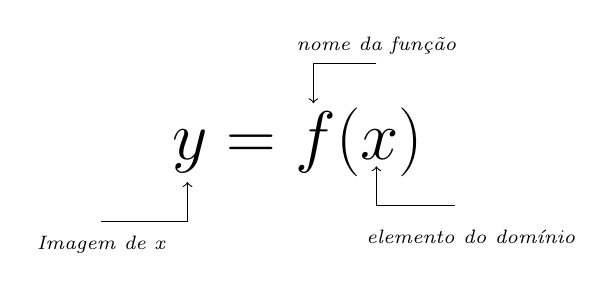
\begin{tikzpicture}
\draw(0,0) node {\Huge $y= f(x)$};
\draw[->](-2.5, -1)--(-1.4,-1)--(-1.4, -.5);
\draw(-2.5,-1.3) node {\em\scriptsize  Imagem de x};
\draw[->](1,1)--(.2,1)--(.2,.5);
\draw (1, 1)node[above]{\em \scriptsize nome da fun\c{c}\~ao};
\draw[->](2,-.8)--(1,-.8)--(1,-.3);
\draw (2.2,- 1.4)node[above]{\em \scriptsize elemento do dom\'{i}nio};
\end{tikzpicture}
\end{figure}

O conjunto \(A\) é chamado \index{domínio da função}domínio da função \(f\), o conjunto \(B\) é chamado \index{contradomínio}contradomínio de \(f\) e o subconjunto de \(B\) formado pelas imagens de todos os elementos de \(A\) é chamado \index{conjunto imagem}conjunto imagem da função \(f\).

\begin{figure}[H]
\centering


\begin{tikzpicture}
\begin{scope}[scale=.8]
\draw [rotate around={90.:(3.,3.5)},thin,fill=\currentcolor!80,fill opacity=0.1] (3.,3.5) ellipse (2.1 and 1.4);
\draw [rotate around={90.:(7.,3.5)},thin,fill=\currentcolor!80,fill opacity=0.1] (7.,3.5) ellipse (2.1 and 1.4);
\draw [line width=.5pt, rounded corners =10pt](5.3,1.2) rectangle(8.7,5.8) ;
\draw [latex-, shift={(5.,2.)},line width=.5pt]  plot[domain=0.8:2.4,variable=\t]({1.*2.8*cos(\t r)+0.*2.8*sin(\t r)},{0.*2.8*cos(\t r)+1.*2.8*sin(\t r)});
\draw(3,3.5) node { $x$};
\draw(7,3.5) node { $f(x)$};
\draw(4.7,5.2) node { $f$};
\draw(3,6) node { $A$};
\draw(7,6.2) node {$B$};
\end{scope}
\end{tikzpicture}
\end{figure}
De maneira geral, escreve-se:
\begin{equation*}
\begin{split}f:A \to B \\
x \mapsto f(x)\end{split}
\end{equation*}
Por exemplo, na {\hyperref[\detokenize{AF106-0:ativ-funcoes-pluviometria}]{Atividade: Pluviometria no Sistema Cantareira}}, se \(f\) é a função que associa a cada ano-mês o índice de chuva real naquele período, \(f(2014-3)=200\) nos informa que o índice de chuva real observada na região do sistema Cantareira no mês de março do ano de 2014 foi de \(200\) milímetros.

Em uma função \(f\) de \(A\) em \(B\), a dependência estabelecida entre as variáveis \(x \in A\) e \(y \in B\) permite que \(y\) seja identificada como “variável dependente” e \(x\) como  “variável independente”, uma vez que os valores assumidos por \(y\) são determinados em função da variação de \(x\) no domínio. Na atividade “Arranha-céu” por exemplo, a variável independente é aquela que representa os andares e a variável dependente é a altura do andar.

\begin{observation}{}

A definição de uma função \(f\) de \(A\) em \(B\) exige que a cada elemento \(x\in A\) corresponda uma imagem \(y=f(x)\in B\) e que não haja ambiguidade na determinação dessa imagem, ou seja, que ela seja única. Asssim, nem toda relação de \(A\) em {\color{red}\bfseries{}{}`}B é uma função. Por exemplo, a relação que associa a cada pessoa o número de seu telefone não é função, pois a imagem pode não ser única, ou seja, há ambiguidade: algumas pessoas têm mais de um número de telefone. E além disso, nem todas as pessoas têm telefone.
\end{observation}

\begin{reflection}
Junto com seus colegas, reflita sobre a definição que acabamos de ver. Vocês conseguem pensar em outros exemplos de relações do seu dia a dia que possam ser consideradas funções? Descrevam algumas delas e compartilhem com o restante da turma, destacando os conjuntos domínio e contradomínio dessas funções.
\end{reflection}
\newpage

\def\currentcolor{session2}
\begin{objectives}{Colorindo o mapa}
{
\begin{itemize}

\item Identificar, em um contexto, diferentes relações de dependência entre conjuntos de dados.

\item Identificar característica de univocidade (ou não) de uma relação..

\end{itemize}
}{1}{1}
\end{objectives}
\begin{sugestions}{Colorindo o mapa}
{
\begin{itemize}
\item Nível de abstração: \textbf{Processo/Ação}.

\item Nem todos os estudantes vão usar o mesmo critério para a distribuição das cores. Incentive-os a usarem as quatro cores e, no momento da discussão do item (b), chame a atenção para o fato de não haver uma única resposta correta para o item (a).

\item Deixamos a seu critério a escolha da unidade para a velocidade média. Os valores obtidos em km/min podem causar certa estranheza, uma vez que na maioria das situações cotidianas a velocidade é apresentada em km/h.

\end{itemize}
}{1}{1}
\end{sugestions}
\clearmargin
\begin{answer}{Colorindo o mapa}
{
\begin{enumerate}
\item {} 
Uma resposta possível é: associar a cor verde aos tempos de $13$ e $14$ minutos, a cor laranja aos tempos de $15$ e $16$ minutos, vermelha ao tempo de $18$ minutos e a cor vinho ao tempo de $23$ minutos.
\item {} 
Isso se deu pelo fato de haver somente 4 cores disponíveis e, na tabela, haver 6 tempos diferentes de travessia.

\item {} 
A velocidade média é determinada pela razão entre a distância percorrida e o tempo gasto para percorrê-la. Assim, os valores das velocidades médias nos diferentes poríodos do dia são, pela ordem em que aparecem na tabela: $1{,}00$ km/min, $0{,}72$ km/min, $0{,}87$ km/min, $0{,}81$ km/min, $0{,}56$ km/min e $1{,}00$ km/min.

\item {} 
Não. Como a velocidade média é calculada efetuando-se a divisão da distância percorrida pelo tempo gasto no percurso, uma vez que o trecho considerado é o mesmo, diferentes tempos de travessia da ponte irão resultar em velocidades médias diferentes.

\end{enumerate}
}{1}
\end{answer}
\begin{objectives}{É função?}
{
\begin{itemize}

\item Identificar, em um contexto, diferentes relações de dependência entre conjuntos de dados, reconhecendo quais são funções.

\item Identificar a univocidade (ou não) de uma relação.

\end{itemize}
}{1}{2}
\end{objectives}
\begin{sugestions}{É função?}
{
\begin{itemize}
\item Nível de abstração: \textbf{Processo}.

\item Esta é a oportunidade para reforçar as condições que garantem que uma relação é função, em particular, a univocidade.
\end{itemize}
}{1}{2}
\end{sugestions}
\begin{answer}{É função?}
{
Apenas as relações de $B$ em $A$ e de $B$ em $C$ não são funções. A primeira porque a uma mesma cor estão associados diferentes tempos de travessia, e a segunda porque a uma mesma cor estão assiciadas velocidades médias diferentes.

}{1}
\end{answer}
\clearmargin
\begin{objectives}{Não é função!}
{
\begin{itemize}

\item Identificar a univocidade (ou não) em uma relação

\end{itemize}
}{1}{1}
\end{objectives}
\marginpar{\vspace{-2em}}
\begin{sugestions}{Não é função!}
{
\begin{itemize}
\item Nível de abstração: \textbf{Processo}.

\item Esta é a oportunidade para reforçar as condições que garantem que uma relação é função, em particular, a univocidade.
\end{itemize}
}{1}{1}
\end{sugestions}
\begin{answer}{Não é função!}
{
\begin{enumerate}
\item {} 
$(2,8),(3,9), (1,1)$ e $(5,10)$ pertencem à relação.

\item {} 
Por exemplo, os pares $(3,12)$ e $(3,15)$ pertencem à relação e isso nos mostra que o número natural $3$ está associado a $12$ e a $15$. Portanto, a relação não pode ser função.

\item {} 
Infinitos.

\item {} 
Um exemplo não númerico: a relação associa cada livro ao seu autor

\end{enumerate}
}{1}
\end{answer}

\begin{objectives}{A família!}
{
\begin{itemize}

\item Identificar uma relação a partir de sua representação no plano cartesiano.

\item Identificar a univocidade (ou não) de uma relação a partir de sua representação no plano cartesiano.

\end{itemize}

}{1}{1}
\end{objectives}
\marginpar{\vspace{-2em}}
\begin{sugestions}{A família!}
{
\begin{itemize}
\item Nível de abstração \textbf{Processo}.

\item No item (b) o objetivo é que os estudantes percebam que, como as pessoas representadas pelos pontos $C$ (Márcia) e $D$ (Júlio) têm a mesma idade mas alturas diferentes, a relação apresentada no gráfico, que associa a idade com a altura nessa ordem, não é função.
\end{itemize}
}{1}{1}
\end{sugestions}
\begin{answer}{A família!}
{
\begin{enumerate}
\item O ponto $A$ representa o bebê Miguel, ponto $B$ Sofia, ponto $C$ Márcia, $D$ Júlio, $E$ Antônio e o ponto $F$ Laura.

\item Não é função, pois Márcia e Júlio têm a mesma idade mas alturas diferentes; no plano, os pontos $C$ e $D$ têm a mesma abscissa e ordenadas diferentes.

\end{enumerate}
}{1}
\end{answer}
\clearmargin
\begin{objectives}{Praticando a notação}
{
\begin{itemize}

\item Compreender funções a partir de sua representação analítica.


\end{itemize}
}{1}{1}
\end{objectives}
\begin{sugestions}{Praticando a notação}
{
\begin{itemize}
\item Nível de abstração: \textbf{Ação}.

\item Muitos estudantes cometem erros relacionados ao uso da expressão analítica que representa a função. É comum, por exemplo, que o cálculo de $f(-2)$ para $f(x)=x^2$ seja feito da seguinte forma: $f(-2)=-2^2=-4$. O que claramente está errado. Muito frequentemente, esse tipo de erro está relacionado à falta de compreensão do papel de uma varíavel em uma expressão algébrica. Aproveite a atividade para fazer uma revisão.
\end{itemize}
}{1}{1}
\end{sugestions}
\begin{answer}{Praticando a notação}
{
\begin{table}[H]
\centering
\begin{tabu} to \textwidth{|l|>{$}c<{$}|}
\hline
\cellcolor{\currentcolor!80}\textcolor{white}{\textbf{Função}} & $\cellcolor{\currentcolor!80}\textcolor{white}{\textbf{Valor}}$ \\
\hline
\(f(3)\) & 42\\ 
\hline
\(g(-1)\) & -1\\
\hline
\(k(2)\) & 6\\
\hline
\(f(1)+g(1)\) & 8\\
\hline
\(g(2)-k(-1)\) & -\frac{46}{3}\\
\hline
\(k(0).f(-2)\) & 20\\
\hline
\(f(0)+h(0)-1\) & -8\\
\hline
\(f(-2).g(-2)+k(2)\) & \frac{36}{5}\\
\hline
\(\dfrac{f(-3)}{k(0)}\) & \frac{6}{5}\\
\hline
\(x\) quando \(h(x)=0\) & \frac{7}{2}\\
\hline
\(x\) quando \(h(x)=3\) & 5\\
\hline
\end{tabu}
\end{table}
}{1}
\end{answer}
\clearmargin
\begin{objectives}{Enchendo o cone}
{
\begin{itemize}

\item Determinar valores da imagem (respectivamente, do domínio) de uma função a partir da sua expressão analítica e de ponto do domínio (respectivamente, da imagem).

\item Interpretar valores do domínio e da imagem de uma função dada que modela uma situação real específica.

\end{itemize}
}{1}{2}
\end{objectives}
\marginpar{\vspace{-2em}}
\begin{sugestions}{Enchendo o cone}
{
\begin{itemize}
\item Nível de abstração \textbf{Ação}.

\item É importante que o estudante identifique a relação existente entre a altura do nível da água no reservatório e o volume do mesmo.

\item Essa pode também ser uma oportunidade para explorar conversão de unidades. Sabemos que a expressão $V=\frac{1}{3}(\pi r^2)h$ fornece o volume do cone em função do raio $r$ e da altura $h$ do nível de água, desde que raio e altura estejam expressos na mesma unidade. A partir das dimensões dadas no enunciado, tem-se $r=\frac{h}{2}$ e, portanto, $V(h)=\frac{1}{3}\pi\frac{h^3}{4}$ é o volume de água no reservatório, em metros cúbicos, correspondente a uma altura de $h$ em metros. Considerando $3$ como aproximação de $\pi$ obtem-se que o volume, em metros cúbicos, é dado, aproximadamente, por $V(h)=\frac{h^3}{4}$, o que equivale em litros a $V(h)=250h^3$.

\item Destaque a “não proporcionalidade” da situação, observando por exemplo, que $2$ é a metade de $4$, mas $2000$ não é a metade de $16000$.
\end{itemize}
}{1}{2}
\end{sugestions}
\marginpar{\vspace{-2em}}
\begin{objectives}{Uniformemente variado}
{
\begin{itemize}

\item Compreender funções a partir de sua representação analítica, relacionando-a ao contexto descrito pelo problema.

\end{itemize}
}{1}{2}
\end{objectives}

\begin{sugestions}{Uniformemente variado}
{
\begin{itemize}
\item Nível de abstração: \textbf{Ação}.

\item Chamar atenção do estudante para o importante papel que as funções desempenham na Física, em especial na Mecânica Clássica, relacionando grandezas como tempo, deslocamento, velocidade e aceleração.
\end{itemize}
}{0}{1}
\end{sugestions}
\begin{answer}{Enchendo o cone}
{
\begin{enumerate}

\item $V(2)$, $V(3)$ e $V(4)$ são, respectivamente iguais a $2000, 6750$ e $16000$ litros e correspondem aos volumes quando a altura da água no reservatório é igual a $2,3$ e $4$ metros, respectivamente.

\item O menor volume observado é $V=0$ litros, que corresponde a $h=0$m, e o maior volume é $V(6)=54000$ litros.

\item Corresponde a uma altura de $2,4$ metros.

\end{enumerate}

\tcbsubtitle{Uniformemente variado}

\begin{enumerate}
\item Inicialmente o veículo está posicionado a $S(0)=2$ quilômetros da origem $O$.

\item Após $4$ horas.

\end{enumerate}
}{0}
\end{answer}


\practice{Conceito do Função}
\vspace{-2\parskip}
\begin{task}{ colorindo o mapa}
\label{\detokenize{AF106-2:atividade-colorindo-o-mapa}}\label{\detokenize{AF106-2:ativ-funcoes-colorindo-o-mapa}}


A imagem a seguir, que foi retirada do aplicativo Google Maps, exibe o trânsito na ponte Rio-Niterói e seus acessos em um determinado dia e hora. Várias informações podem ser observadas a partir dos elementos apresentados. Por exemplo, as cores nas vias informam a velocidade média dos veículos que trafegam por elas, conforme a legenda na parte inferior; a distância entre dois pontos quaisquer do mapa pode ser estimada usando a escala exibida no canto inferior direito. Gráficos como esse são produzidos a partir das relações entre diversas informações coletadas.

\begin{figure}[H]
\centering

\noindent\includegraphics[width=425bp]{{rio_niteroi_maps}.png}
\end{figure}

A tabela a seguir mostra os dados coletados sobre o tempo gasto pelos veículos (em média) para atravessar a ponte, ao longo de um dia.

\begin{table}[H]
\centering

\begin{tabu} to \textwidth{|c|c|>{\centering}m{.1\textwidth}|c|}
\hline
\thead
Período do Dia & Tempo (min) & Cor & Velocidade Média (km/min) \\
\hline
5:00 - 7:00 & 13 & & \\
\hline
7:00 - 9:00 & 18 & & \\
\hline
9:00 - 11:00 & 15 & & \\
\hline
11:00 - 13:00 & 15 & & \\
\hline
13:00 - 15:00 & 16 & & \\
\hline
15:00 - 17:00 & 16 & & \\
\hline
17:00 - 19:00 & 23 & & \\
\hline
19:00 - 21:00 & 14 & & \\
\hline
21:00 - 23:00 & 13 & & \\
\hline
\end{tabu}
\end{table}

\begin{enumerate}
\item {} 
Tomando como referência a ilustração anterior e utilizando a escala de cores a seguir, complete a terceira coluna da tabela com a cor que a ponte deveria estar colorida em cada período do dia destacado. Descreva os critérios que você utilizou na escolha de cada uma das cores e compare com os critérios dos seus colegas.
\begin{center}\begin{tikzpicture}[scale=3]
\tikzset{fontscale/.style = {font=\relsize{#1}}}
\fill[fill=green] (3.,1.) rectangle (3.6,1.2);
\fill[fill=orange] (3.65,1.) rectangle (4.25,1.2);
\fill[fill=red] (4.3,1.) rectangle (4.9,1.2);
\fill[fill=brown] (4.95,1.) rectangle (5.55,1.2);
\node[below left, font=\small] at (3,1.15) {RÁPIDO};
\node[below right, font=\small] at (5.55,1.15) {LENTO};
\node at ($(3,1)!0.5!(3.6,1.2)$) {verde};
\node at ($(3.65,1)!0.5!(4.25,1.2)$) {laranja};
\node at ($(4.3,1)!0.5!(4.9,1.2)$) {vermelho};
\node at ($(4.95,1)!0.5!(5.55,1.2)$) {marrom};
\end{tikzpicture}\end{center}
\item {} 
Você precisou associar uma mesma cor para para períodos diferentes do dia. Por que?

\item {} 
Sabendo que a ponte Rio-Niterói tem aproximadamente \(13\) km de extensão complete a quarta coluna da tabela com a velocidade média registrada em cada um dos períodos do dia.

\item {} 
É possível que uma mesma velocidade média esteja associada a dois tempos de travessia diferentes? Por quê?
\end{enumerate}
\end{task}

Na atividade anterior, observam-se diferentes relações entre os dados. Por exemplo, para cada tempo de travessia é possível associar uma única cor e uma única velocidade média. Da mesma maneira, a cada velocidade média está associada uma única cor e um único tempo de travessia. No entanto, a uma mesma cor é possível associar tempos diferentes e velocidades médias diferentes.

\begin{task}{ é função?}
\label{\detokenize{AF106-2:atividade-e-funcao}}\label{\detokenize{AF106-2:ativ-funcoes-e-funcao}}

No contexto da atividade anterior são observados diferentes conjuntos de dados: O conjunto dos tempos de travessia da ponte, \(A=\{13, 14, 15, 16, 18, 23\}\); O conjunto das cores que compoõem a escala, \(B=\{\)Verde, Laranja, Vermelho, Vinho\(\}\); e o conjunto de velocidades obtidas,{}`C{}`. Considere as diferentes relações de dependências estabelecidas entre esses conjuntos. Quais são funções?

\begin{table}[H]
\centering
\begin{tabu} to \textwidth{|c|c|>{\centering}m{6cm}|}
\hline
\thead
Relação & É função? &  Se não, por que? \\
\hline
De A em B
&&\\
\hline
De B em A
&&\\
\hline
De A em C
&&\\
\hline
De C em A
&&\\
\hline
De B em C
&&\\
\hline
De C em B
&&\\
\hline
\end{tabu}
\end{table}
\end{task}

Toda relação de um conjunto \(A\) em um conjunto \(B\) pode ser identificada por um conjunto de pares ordenados. Nesse caso, cada associação entre elementos do conjunto \(A\) e elementos do conjunto \(B\) fica representada por um par ordenado tal que o elemnto do conjunto \(A\) ocupa a primeira posição do par e o correspondente elemento do conjunto \(B\) a segunda posição.

Por exemplo, se consideramos a relação dos números reais em si mesmo que, a cada número real, associa o seu quadrado, os pares ordenados \((1,1), (2,4), (\sqrt{3},3), (-\pi,\pi^2)\) indicam elementos que estão relacinados. Já os pares ordenados \((9,5)\) e \((4,2)\), \((\sqrt{2},-2)\) formados por números reais, não indicam números associados pela mesma relação, uma vez que \(5\) não é quadrado de \(9\), \(2\) não é quadrado de \(4\) e \(-2\) não é o quadrado de \(\sqrt{2}\).

Como funções são um tipo especial de relação, a mesma ideia se estende para representação das funções. Assim, os pares ordenados de uma função \(f:A\to B\) serão da forma \((x,y)\) em que \(x\in A\) e \(y=f(x)\in B\).


\begin{task}{ não é função!}
\label{\detokenize{AF106-2:atividade-nao-e-funcao}}\label{\detokenize{AF106-2:ativ-funcoes-nao-e-funcao}}

Considere a relação formada por todos \((a,b)\) de números naturais tais que \(b\) é múltiplo de \(a\). Assim, \((2,4)\), \((2,6)\), \((3,6)\) e \((9, 9)\) são pares ordenado dessa relação, pois \(4\) é múltiplo de \(2\), \(6\) é múltiplo de \(2\) e de \(3\) e \(9\) é múltiplo de \(9\) . No entanto, \((4,2)\) e \((7,17)\) são pares ordenados de números naturais, mas não são pares dessa relação.
\begin{enumerate}
\item {} 
Exiba outros quatro pares ordenados dessa relação.

\item {} 
Explique porque essa relação não é uma função.

\item {} 
\((5, 405)\) é um par ordenado dessa relação. Quantos outros pares ordenados dessa relação têm 5 como primeiro elemento?

\item {} 
Dê exemplo de uma ou mais relações que não sejam funções. Não precisam ser exemplos numéricos.

\end{enumerate}
\end{task}

\begin{task}{ a família}
\label{\detokenize{AF106-2:atividade-a-familia}}

Cada ponto do gráfico a seguir representa uma das seguintes pessoas.

\begin{figure}[H]
\centering

\noindent\includegraphics[width=300bp]{{familia}.png}
\label{\detokenize{AF106-2:fig-altura-idade}}
\end{figure}

\begin{enumerate}
\item {} 
Associe cada ponto do gráfico à pessoa correspondente.

\item {} 
A relação expressa pelos pares ordenados (idade, altura) apresentados no gráfico é função? Por que?
\end{enumerate}


\begin{center}\begin{tikzpicture}[scale=1.4]
\draw[->](-0,0)--(6,0);
\draw(5.7,0) node [below]{idade};
\draw[->](0,-0)--(0,4);
\draw(0,3.95) node [above left, rotate =90]{altura};
\draw[fill](5.5,1.5) circle(1pt) node[right]{$F$};
\draw[dotted] (5.5,0)--(5.5,1.5)--(0,1.5);
\draw[fill](4.5,3.5) circle(1pt) node[above]{$E$};
\draw[dotted](4.5,0)--(4.5,3.5)--(0,3.5);
\draw[fill](3,3.5) circle(1pt) node[above]{$D$};
\draw[dotted](3,0)--(3,3.5);
\draw[fill](3,2.5) circle(1pt) node[right]{$C$};
\draw[dotted](3,2.5)--(0,2.5);
\draw[fill](2,1) circle(1pt) node[right]{$B$};
\draw[dotted](2,0) -- (2,1) --(0,1);
\draw[fill](.5,.3) circle(1pt) node[right]{$A$};
\draw[dotted](.5,0)--(.5,.3)--(0,.3);
\end{tikzpicture}\end{center}




{\color{red}\bfseries{}*}Adaptado de The Language of Functions and Graphs, Shell Centre for Mathematical Education Publications Ltd., 1985.
\end{task}

Quando nos deparamos com uma função é fundamental identificarmos os conjuntos domínio e contradomínio, e a maneira como os elementos desses conjuntos estão relacionados. Tal maneira pode ser muito variada, no entanto, principalmente quando os conjuntos envolvidos são numéricos, é comum considerar como contradomínio o conjunto \(\mathbb{R}\). Por isso, daqui por diante, quando estivermos considerando funções numéricas, o contradomínio será igual a \(\mathbb{R}\).

Em muitos casos, a forma de associação entre os elementos é dada por uma expressão analítica. Vejamos alguns exemplos.

\((I)\) Para calcular o perímetro de um quadrado de lado \(\ell\) usa-se a expressão \(P=4\ell\). Percebe-se então que o perímetro está relacionado com o lado. A partir daí pode-se definir a função perímetro:
\begin{equation*}
\begin{split}P: ]0,+\infty[\to \mathbb{R} \quad ; \quad P(\ell)=4\ell.\end{split}
\end{equation*}
Da mesma forma a área de um quadrado de lado \(\ell\) é dada por \(A=\ell^2\), que permite definir a função:
\begin{equation*}
\begin{split}A: ]0,+\infty[\to \mathbb{R} \quad ; \quad A(\ell)=\ell^2.\end{split}
\end{equation*}
A variável \(\ell\) pode assumir qualquer valor dentro do intervalo \(]0,+\infty[\) que é o domínio da função \(P\) . Se quisermos saber o valor do perímetro do quadrado de lado $5$cm, basta substituirmos \(\ell\) por 5 na expressão de  \(P(\ell)\). Ficamos assim com
\begin{equation*}
\begin{split}P(5)=4\times 5 = 20\mathrm{cm}.\end{split}
\end{equation*}
A área do quadrado de lado $9$cm é
\begin{equation*}
\begin{split}A(9)=9^2=81\text{cm}^2.\end{split}
\end{equation*}
\((II)\) A fórmula de Lorentz já foi muito utilizada pelos médicos para o cálculo do “peso ideal” \(p\), em kg, em função da altura \(h\), em centímetros, do paciente.
\begin{equation*}
\begin{split}p:]0,300[\to \mathbb{R}\quad ; \quad p(h)=h-100-\dfrac{h-150}{k}\end{split}
\end{equation*}
em que \(k\) vale 4 para homens e vale 2 para mulheres.

Que tal usar a fórmula acima para calcular o seu peso ideal?

\((III)\) Imagine que um objeto é solto, a partir do repouso, de uma altura de \(10\) metros e percorre uma trajetória vertical em queda livre. Da Física, sabemos que sua altura \(h\) em metros medida a partir do solo, em função do tempo \(t\) em segundos, quando desprezamos a resistência do ar, é dada por
\begin{equation*}
\begin{split}h:[0,+\infty[\to \mathbb{R}\quad ; \quad h(t)=10-\dfrac{gt^2}{2},\end{split}
\end{equation*}
em que \(g\) representa a aceleração da gravidade em \(m/s^2\).metros por segundo ao quadrado.

Fazer a variável tempo assumir o valor \(t=0\) segundos na expressão de \(h(t)\) significa que estamos medindo a altura no início da contagem do tempo, ou seja a altura inicial do corpo. Nesse caso teremos
\begin{equation*}
\begin{split}h(0)=10-\dfrac{g\ 0^2}{2}=10.\end{split}
\end{equation*}
\emph{Se por exemplo, quisermos saber em quanto tempo o corpo chegará ao solo, o que devemos fazer?} Como a medição é feita a partir do solo, dizer que o objeto chegou ao solo é o mesmo que dizer que sua altura é igual a 0. Portanto, precisamos descobrir o valor da variável \(t\), de maneira que \(h(t)=0\). A partir da expressão de \(h(t)\) e aproximando \(g\) por \(10 m/s^2\), obtemos \(10-5t^2=0\), donde concluímos que  \(t=\sqrt{2}\) aproximadamente.


\begin{task}{ praticando a notação}
\label{\detokenize{AF106-2:atividade-praticando-a-notacao}}\label{\detokenize{AF106-2:ativ-praticando-notacao}}

Considere as funções \(f\), \(g\), \(k\) e \(h\), todas de domínio \(\mathbb{R}\), tais que:
\begin{equation*}
\begin{split}f(x)=3x^2+5x\quad ; \quad g(x)=\frac{x-1}{x^3+3}\quad ; \quad k(x)=(x-2)^2+6\quad ; \quad h(x)=2x-7\end{split}
\end{equation*}
Determine o valor de:


\begin{table}[H]
\centering
\begin{tabu} to \textwidth{|l|c|}
\hline
\thead
Função & Valor \\
\hline
\(f(3)\) & \\ 
\hline
\(g(-1)\) & \\
\hline
\(k(2)\) & \\
\hline
\(f(1)+g(1)\) & \\
\hline
\(g(2)-k(-1)\) & \\
\hline
\(k(0).f(-2)\) & \\
\hline
\(f(0)+h(0)-1\) & \\
\hline
\(f(-2).g(-2)+k(2)\) & \\
\hline
\(\dfrac{f(-3)}{k(0)}\) & \\
\hline
\(x\) quando \(h(x)=0\) & \\
\hline
\(x\) quando \(h(x)=3\) & \\
\hline
\end{tabu}
\end{table}

\end{task}

\begin{task}{ enchendo o cone}
\label{\detokenize{AF106-2:atividade-enchendo-o-cone}}\label{\detokenize{AF106-2:ativ-funcoes-enchendo-o-cone}}

O reservatório representado a seguir tem a forma de um cone cuja altura é \(6 m\) e a base é um círculo de raio \(3 m\). O volume \(V\) em litros de água no reservatório pode ser estimado a partir altura do nível da água \(h\) (em metros) de acordo com a seguinte expressão:
\begin{equation*}
\begin{split}V(h)=250h^3\end{split}
\end{equation*}\begin{center}\begin{tikzpicture}
\fill[thick,color=\currentcolor!80,fill=\currentcolor!80,fill opacity=0.10000000149011612, left color =white, right color =\currentcolor!80] (1.,0.) -- (-0.5,3.) -- (2.5,3.) -- cycle;
\draw [rotate around={-180:(1.0047836744699097,3.1435102340973167)},thick,left color=\currentcolor!80, right color=\currentcolor!80, middle color=white] (1.0047836744699097,3.1435102340973167) ellipse (1.5611029721362464cm and 0.5184113668542463cm);
\draw [rotate around={-180:(1.0071755117048646,4.715265351145975)},thick, left color=gray!80, right color=gray!60, middle color=white] (1.0071755117048646,4.715265351145975) ellipse (2.341654458204363cm and 0.7776170502813675cm);
\draw [thick] (1.,0.)-- (-1.3303743315507686,4.660748663101537);
\draw [thick] (1.,0.)-- (3.347109515260305,4.69421903052061);
\draw[dashed](1,0) -- (3.4,0);
\draw[|-|, dashed](2.6,0)--(2.6,3);
\draw (2.7,1.6) node[right] {$h$};
\draw[|-|, dashed](3.4,0)--(3.4,4.6);
\draw (3.5,2) node[right] {6 m};
\end{tikzpicture}\end{center}\begin{enumerate}
\item {} 
Determine \(V(2), V(3)\) e \(V(4)\) e explique os seus significados no contexto.

\item {} 
Quais os volumes de água, mínimo e máximo, que o reservatório comporta?

\item {} 
A que altura do nível da água corresponde o volume igual a \(3 456\) litros?

\end{enumerate}
\end{task}

\begin{task}{ uniformemente variado}
\label{\detokenize{AF106-2:atividade-uniformemente-variado}}\label{\detokenize{AF106-2:ativ-funcoes-uniformemente-variado}}

A posição \(S\) (em quilômetros), medida a partir de um referencial, de um veículo que se desloca segundo um movimento retilíneo uniformemente variado (MRUV) é dada em função do tempo \(t\) (medido em horas) pela seguinte expressão:
\begin{equation*}
\begin{split}S(t)=2t^2-4t+2\end{split}
\end{equation*}\begin{enumerate}
\item {} 
Determine a posição inicial do veículo. Explique o significado desse resultado a partir do contexto.

\item {} 
Após quanto tempo o veículo estará a $18$km da origem?

\end{enumerate}
\end{task}

\clearpage
\def\currentcolor{session3}
\begin{objectives}{Por que não é função?}
{
\begin{itemize}

\item Identificar em contextos mais variados por que uma dada relação não define uma função.

\end{itemize}
}{1}{2}
\end{objectives}
\begin{sugestions}{Por que não é função?}
{
\begin{itemize}
\item Nível de abstração \textbf{Processo}.

\item Procure incentivar os estudantes a se manifesrem verbalmente, expressando seu entendimento sobre a relação dada. Para a primeira relação, por exemplo, sugerimos que seja considerado, em um primeiro momento, o conjunto formado por todos os estudantes da sala. Possivelmente haverá estudantes sem irmãos e estudantes com mais de um irmão.

\item No item (b) relembre com os alunos que a raiz quadrada é sempre um valor positivo. Por exemplo, $\sqrt{4}=2$. Apesar de a equação $x^2=4$ ter duas soluções: $2$ e $−2$.
\end{itemize}
}{1}{2}
\end{sugestions}
\begin{answer}{Por que não é função?}
{
\begin{enumerate}
\item Como existem filhos únicos no mundo e famílias com mais do que dois filhos, existem "pessoas" no conjunto $\mathcal{P}$ que não têm irmão e pessoas que têm mais do que um irmão. Portanto, pela relação dada, há no conjunto $\mathcal{P}$ elementos sem correspondente bem como elementos com mais do que um correspondente. Por isso, a relação dada não é função.

\item Como não existe $\mathbb{R}$ raiz quadrada de número negativo, a relação dada não se aplica aos números reais negativos, isto é, por exemplo o número real $-1$ não pode ser associado à $\sqrt{-1}$, uma vez que $\sqrt{-1}$ não pertence ao conjunto dos números reais. Portanto, haverá elementos (todos os números reais negativos) sem correspondente. Por isso, a relação dada não é função. Observe que, no entanto, a mesma relação considerada apenas para os números reais não negativos, ou seja, com domínio $\mathbb{R}^+$, seria uma função.

\item Considerando, por exemplo, o número real $15$ é possível construir dois triângulos distintos, ambos com área igual a $15$. Basta considerar para o primeiro base e altura iguais a $5$ e $6$ e para o segundo base e altura iguais a $10$ e $3$, que claramente não são triângulos congruentes. Dessa forma, haverá ambiguidade na determinação de correspondentes. Por isso, a relação dada não é função.

\end{enumerate}
}{0}
\end{answer}
\begin{objectives}{Domínio e imagem}
{
\begin{itemize}

\item Determinar a partir da expressão algébrica os conjuntos domínio e imagem.

\end{itemize}
}{1}{2}
\end{objectives}
\begin{sugestions}{Domínio e imagem}
{
\begin{itemize}
\item Nível de abstração: \textbf{Ação}.

\item É importante que o estudante perceba as restrições para a escolha de $x$ impostas por algumas das expressões dadas.
\end{itemize}
}{1}{2}
\end{sugestions}
\begin{answer}{Domínio e imagem}
{
Ajude o estudante a completar a tabela.

\begin{table}[H]
\centering
\begin{tabu} to \textwidth{|c|c|c|}
\hline
\thead
Expressão & Domínio $A$ & Imagem \\
\hline
\((a)\) & \(\mathbb{R}^+\) & $\mathbb{R}^+$\\
\hline
\((b)\) & $[5,+\infty[$ & $\mathbb{R}^+$\\
\hline
\((c)\) & $\mathbb{R}\setminus\{3\}$ & \(\mathbb{R}\setminus \{0\}\) \\
\hline
\((d)\) & \(\mathbb{R}\setminus \{-8\}\) & $\mathbb{R}\setminus\{0\}$ \\
\hline
\((e)\) & $]0,+\infty[$ & $]0,+\infty[$ \\ 
\hline
\((f)\) & $\mathbb{R}$ & \([7,+\infty[\) \\
\hline
\((g)\) & $\mathbb{R}$  & $[8,+\infty[$ \\
\hline
\((h)\) & $\mathbb{R}$  & $[-3,+\infty[$ \\
\hline
\end{tabu}
\end{table}
}{1}
\end{answer}

\know{}
\label{\detokenize{AF106-3::doc}}\label{\detokenize{AF106-3:sec-aprofundando}}\label{\detokenize{AF106-3:para-saber-mais}}

\begin{task}{ por que não é função?}
\label{\detokenize{AF106-3:ativ-nao-funcao}}\label{\detokenize{AF106-3:atividade-por-que-nao-e-funcao}}

Vimos que para que uma relação de \(A\) em \(B\) seja uma função não pode haver:

\((I)\) Elementos no conjunto \(A\) sem correspondente em \(B\);
\((II)\) Ambiguidade na determinação de correspondente em \(B\).

Determine se cada uma das relações apresentadas a seguir é função. Justifique suas respostas a partir das condições \((I)\) e \((II)\).
\begin{enumerate}
\item {} 
Seja \(\mathcal{P}\) o conjunto de todas as pessoas e considere a relação de \(\mathcal{P}\) em \(\mathcal{P}\), que a cada “pessoa” associa “irmão da pessoa”.

\item {} 
Seja \(\mathbb{R}\)  o conjunto dos números reais e considere a relação de \(\mathbb{R}\) em \(\mathbb{R}\), que a cada “número real \(x\) ” associa “raiz quadrada do número real \(x\) “.

\item {} 
Sejam \(\mathbb{R}^+\) o conjunto dos números reais positivos e \(\mathcal{T}\) o conjunto de todos os triângulos. Considere a relação de \(\mathbb{R}^+\) em \(\mathcal{T}\) que a cada “número real positivo \(x\) ” associa “triângulo de área \(x\) “.

\end{enumerate}

\end{task}

\begin{task}{ domínio e imagem}
\label{\detokenize{AF106-3:ativ-qual-e-imagem}}\label{\detokenize{AF106-3:atividade-dominio-e-imagem}}

Considere a seguinte lista de expressões algébricas.
\begin{multicols}{3}
\begin{enumerate}
\item {} 
\(f(x)=\sqrt{x}\)

\item {} 
\(G(z)=\sqrt{z-5}\)

\item {} 
\(h(s)=\frac{1}{3-s}\)

\item {} 
\(J(t)=\frac{1}{t+8}\)

\item {} 
\(T(x)=\frac{1}{\sqrt{x}}\)

\item {} 
\(R(x)=(x-2)^2+7\)

\item {} 
\(g(u)=5u^2+8\)

\item {} 
\(F(x)=(x+1)^2-3\)

\end{enumerate}
\end{multicols}

Veja que, em algumas das expressões, a variável independente não pode assumir alguns valores, por exemplo, na letra a) \(x\) não pode assumir valores negativos. Complete a tabela abaixo com o maior conjunto domínio possível que cada uma das funções pode ter e o correspondente conjunto imagem.


\begin{table}[H]
\centering
\begin{tabu} to \textwidth{|c|c|c|}
\hline
\thead
Expressão & Domínio $A$ & Imagem \\
\hline
\((a)\) & \(\mathbb{R}^+\) & \\
\hline
\((b)\) & & \\
\hline
\((c)\) & & \(\mathbb{R}\setminus \{0\}\) \\
\hline
\((d)\) & \(\mathbb{R}\setminus \{-8\}\) & \\
\hline
\((e)\) & & \\ 
\hline
\((f)\) & & \([7,+\infty[\) \\
\hline
\((g)\) & & \\
\hline
\((h)\) & & \\
\hline
\end{tabu}
\end{table}


\end{task}

\exercise

\begin{answer}{Exercícios}
{\exerciselist
  \begin{enumerate}
  \item 
  \begin{enumerate}
  \item \adjustbox{valign=t}
  {\resizebox{.95\linewidth}{!}
  {
  
    
\begin{tikzpicture}
    \draw [fill] (0.,0.) circle (.5pt);
    \draw [fill] (0.2,0.) circle (.5pt);
    \draw [fill] (0.2,0.2) circle (.5pt);
    \draw [fill] (0.,0.2) circle (.5pt);
    \draw [fill] (0.4,0.) circle (.5pt);
    \draw [fill] (0.4,0.4) circle (.5pt);
    \draw [fill] (0.,0.4) circle (.5pt);
    \draw [fill] (0.6,0.) circle (.5pt);
    \draw [fill] (0.6,0.6) circle (.5pt);
    \draw [fill] (0.,0.6) circle (.5pt);
    \draw [fill] (0.8,0.) circle (.5pt);
    \draw [fill] (0.8,0.8) circle (.5pt);
    \draw [fill] (0.,0.8) circle (.5pt);
    \draw [fill] (0.4,0.2) circle (.5pt);
    \draw [fill] (0.2,0.4) circle (.5pt);
    \draw [fill] (0.6,0.2) circle (.5pt);
    \draw [fill] (0.6,0.4) circle (.5pt);
    \draw [fill] (0.4,0.6) circle (.5pt);
    \draw [fill] (0.2,0.6) circle (.5pt);
    \draw [fill] (0.8,0.2) circle (.5pt);
    \draw [fill] (0.8,0.4) circle (.5pt);
    \draw [fill] (0.8,0.6) circle (.5pt);
    \draw [fill] (0.6,0.8) circle (.5pt);
    \draw [fill] (0.4,0.8) circle (.5pt);
    \draw [fill] (0.2,0.8) circle (.5pt);
    \begin{scope}[xshift=1.3cm]
    \draw [fill] (0.,0.) circle (.5pt);
    \draw [fill] (0.2,0.) circle (.5pt);
    \draw [fill] (0.2618033988749895,0.19021130325903063) circle (.5pt);
    \draw [fill] (0.1,0.3077683537175253) circle (.5pt);
    \draw [fill] (-0.06180339887498945,0.19021130325903074) circle (.5pt);
    \draw [fill] (0.4,0.) circle (.5pt);
    \draw [fill] (0.523606797749979,0.38042260651806126) circle (.5pt);
    \draw [fill] (0.2,0.6155367074350506) circle (.5pt);
    \draw [fill] (-0.1236067977499789,0.3804226065180615) circle (.5pt);
    \draw [fill] (0.6,0.) circle (.5pt);
    \draw [fill] (0.7854101966249685,0.570633909777092) circle (.5pt);
    \draw [fill] (0.3,0.9233050611525759) circle (.5pt);
    \draw [fill] (-0.18541019662496844,0.5706339097770922) circle (.5pt);
    \draw [fill] (0.8,0.) circle (.5pt);
    \draw [fill] (1.047213595499958,0.7608452130361225) circle (.5pt);
    \draw [fill] (0.4,1.2310734148701012) circle (.5pt);
    \draw [fill] (-0.2472135954999578,0.760845213036123) circle (.5pt);
    \draw [fill] (0.4618033988749895,0.19021130325903063) circle (.5pt);
    \draw [fill] (0.3618033988749895,0.49797965697655594) circle (.5pt);
    \draw [fill] (0.038196601125010596,0.49797965697655605) circle (.5pt);
    \draw [fill] (0.6618033988749895,0.19021130325903068) circle (.5pt);
    \draw [fill] (0.7236067977499789,0.3804226065180614) circle (.5pt);
    \draw [fill] (0.6236067977499793,0.6881909602355865) circle (.5pt);
    \draw [fill] (0.4618033988749902,0.8057480106940809) circle (.5pt);
    \draw [fill] (0.1381966011250101,0.8057480106940811) circle (.5pt);
    \draw [fill] (-0.023606797749979813,0.6881909602355861) circle (.5pt);
    \draw [fill] (0.86180339887499,0.19021130325903102) circle (.5pt);
    \draw [fill] (0.9236067977499794,0.38042260651806226) circle (.5pt);
    \draw [fill] (1.0075247947399484,0.5619653557018063) circle (.5pt);
    \draw [fill] (0.8831438349325862,0.880048871647975) circle (.5pt);
    \draw [fill] (0.7190740743652143,0.9992525302598276) circle (.5pt);
    \draw [fill] (0.5550043137978428,1.1184561888716802) circle (.5pt);
    \draw [fill] (0.24674654820709388,1.1160849093529024) circle (.5pt);
    \draw [fill] (0.09375519577774943,1.0007479119524167) circle (.5pt);
    \draw [fill] (-0.06488577814196421,0.8933141263850993) circle (.5pt);
    \begin{scope}[xshift=1.7cm]
    \draw [fill] (0.,0.) circle (0.5pt);
    \draw [fill] (0.2,0.) circle (0.5pt);
    \draw [fill] (0.3,0.17320508075688776) circle (0.5pt);
    \draw [fill] (0.2,0.34641016151377557) circle (0.5pt);
    \draw [fill] (0.,0.3464101615137756) circle (0.5pt);
    \draw [fill] (-0.1,0.1732050807568879) circle (0.5pt);
    \draw [fill] (0.4,0.) circle (0.5pt);
    \draw [fill] (0.6,0.3464101615137755) circle (0.5pt);
    \draw [fill] (0.4,0.6928203230275511) circle (0.5pt);
    \draw [fill] (0.,0.6928203230275513) circle (0.5pt);
    \draw [fill] (-0.2,0.3464101615137758) circle (0.5pt);
    \draw [fill] (0.6,0.) circle (0.5pt);
    \draw [fill] (0.9,0.5196152422706631) circle (0.5pt);
    \draw [fill] (0.6,1.0392304845413265) circle (0.5pt);
    \draw [fill] (0.,1.0392304845413265) circle (0.5pt);
    \draw [fill] (-0.3,0.5196152422706637) circle (0.5pt);
    \draw [fill] (0.8,0.) circle (0.5pt);
    \draw [fill] (1.2,0.692820323027551) circle (0.5pt);
    \draw [fill] (0.8,1.3856406460551023) circle (0.5pt);
    \draw [fill] (0.,1.3856406460551025) circle (0.5pt);
    \draw [fill] (-0.4,0.6928203230275516) circle (0.5pt);
    \draw [fill] (0.5,0.17320508075688776) circle (0.5pt);
    \draw [fill] (0.5,0.5196152422706634) circle (0.5pt);
    \draw [fill] (0.4,0.6928203230275511) circle (0.5pt);
    \draw [fill] (0.2,0.6928203230275511) circle (0.5pt);
    \draw [fill] (-0.1,0.5196152422706635) circle (0.5pt);
    \draw [fill] (0.7,0.1732050807568877) circle (0.5pt);
    \draw [fill] (0.8,0.34641016151377546) circle (0.5pt);
    \draw [fill] (0.8,0.6928203230275509) circle (0.5pt);
    \draw [fill] (0.7,0.8660254037844384) circle (0.5pt);
    \draw [fill] (0.4,1.0392304845413265) circle (0.5pt);
    \draw [fill] (0.2,1.0392304845413265) circle (0.5pt);
    \draw [fill] (-0.1,0.8660254037844397) circle (0.5pt);
    \draw [fill] (-0.2,0.6928203230275531) circle (0.5pt);
    \draw [fill] (0.9,0.17320508075688779) circle (0.5pt);
    \draw [fill] (1.,0.34641016151377557) circle (0.5pt);
    \draw [fill] (1.1,0.5196152422706637) circle (0.5pt);
    \draw [fill] (1.1,0.8660254037844383) circle (0.5pt);
    \draw [fill] (1.,1.039230484541325) circle (0.5pt);
    \draw [fill] (0.9,1.212435565298211) circle (0.5pt);
    \draw [fill] (0.6,1.385640646055102) circle (0.5pt);
    \draw [fill] (0.4,1.3856406460551023) circle (0.5pt);
    \draw [fill] (0.2,1.3856406460551023) circle (0.5pt);
    \draw [fill] (-0.1,1.2124355652982246) circle (0.5pt);
    \draw [fill] (-0.2,1.0392304845413458) circle (0.5pt);
    \draw [fill] (-0.3,0.8660254037844671) circle (0.5pt);
    \end{scope}
    \end{scope}
    \end{tikzpicture}
  }
  }
  \vspace{.5em}

  \item Para a primeira sequência (números quadrados perfeitos): $1,4,9,16,25,...$, para a segunda sequência (números pentagonais): $1,5,12,22,35,...$ e para a terceira sequência (números hexagonais): $1,6,15,28,45,...$

  \item Uma resposta possível: 

  \begin{itemize}
  \item O $n$-ésimo número quadrado perfeito é da forma $n^2$.
  
  \item Denotando por $P_n$ o $n$-ésimo número pentagonal, temos $P_{n+1}=P_n+(3(n-1)+4)$, ou ainda, $P_n=\dfrac{3n^2-n}{2}$.

  \item Denotando por $H_n$ o $n$-ésimo número hexagonal, temos $H_{n+1}=H_n+(4(n-1)+5)$, ou ainda, $H_n=2n^2-n$.
  \end{itemize}
  \end{enumerate}

  \end{enumerate}
}{1}
\end{answer}
\clearmargin
\begin{answer}{Exercícios}
{\exerciselist
  \begin{enumerate}\setcounter{enumi}{1}
  \item 
  \begin{enumerate}
  \item Na primeira sequência observa-se que o número seguinte é obtido pela soma dos dois números anteriores a ele. A sequência obtida dessa forma é conhecida como \textit{Sequência de Fibonacci}. Na segunda sequência nota-se que o número seguinte é obtido dividindo-se o anterior por $10$
  \item Na primeira, o vigésimo termo é $6765$ e na segunda $10^{-16}$.
  \end{enumerate}


  \item
  \begin{enumerate}
  \item O prisma seguinte é obtido a partir do anterior pela adição de $4$ cubos cinzas à pilha de cubos cinzas já existente.
  \item São necessários $16$ cubos cinzas.
  \item O número de cubos cinzas em qualquer um dos primas da sequência será sempre um múltiplo de $4$, e portanto um número par.
  \item O prisma $200$ terá $200\cdot4=800$ cubos cinzas.
  \item O prisma $n$ terá $n\cdot4$ cubos cinzas.
  \item A expressão $4n$, que fornece o número de cubos cinzas no Prisma $n$, é um número par qualquer que seja o valor de $n$ considerado.
  \item Cada Prisma da sequência possui $8$ cubos brancos, sendo assim, se $x$ representa o total de cubos (brancos e cinzas), então o número de cubox cinzas será dado por $x-8$.
  \end{enumerate}
  \end{enumerate}
}{1}
\end{answer}
\clearmargin
\begin{answer}{Exercícios}
{\exerciselist
  \begin{enumerate}\setcounter{enumi}{3}
  \item 
  \begin{enumerate}
  \item Ela gastou $6$s
  \end{enumerate}
  \item
  As duas primeiras afirmações são falsas, pois Ana prcorreu $\dfrac{4}{5}$ (mais da metade) da distância correndo e o $\dfrac{1}{5}$ restante andando. A terceira afirmação é falsa, uma vez que Ana correu durante $\dfrac{1}{4}$  do tempo apenas. De acordo com o gráfico, a quarta afirmação é verdadeira.
  \end{enumerate}
}{1}
\end{answer}
\clearmargin
\begin{answer}{Exercícios}
{\exerciselist
  \begin{enumerate}\setcounter{enumi}{5}
  \item 
  \begin{enumerate}
  \item No mês de janeiro o comprimento do cabelo de Vitor era de $3$cm e no mês de junho $10$cm.
  \item $1{,}4$cm.
  \item $C(M)=3+1{,}4M$
  \item A partir da expressão obtida no item anterior, resolvemos $19{,}8=3+1{,}4M$, obtendo $M=12$ meses.
  \end{enumerate}
  \item
  \begin{enumerate}
  \item $g(\sqrt{10})<g(\sqrt{5})<g(\sqrt{2})$.
  \item $x=1$ e $x=-1$.
  \item Não, pois $g(x)=9-x^2\leq 9$, qualquer que seja o $x\in\R$.
  \item $b$ deveria ser um número real menor ou igual a $9$.
  \end{enumerate}
  \item
  \begin{enumerate}
  \item $1+3+7+1+7=19$
  \item Uma resposta possível é $499$.
  \item Veja que os números $3,30,300,3000,12,120,1200,102,1020,\\1002,111,1101,1011,1110,21,210,201,2001,2100$ e $2010$ são tais que a soma de seus algarismos é igual a $3$ e são todos os números entre $1$ e $10000$ com essa propriedade. Portanto há 20 números com a propriedade requerida.
  \item Sim. Dado um número natural $n$, basta considerar o número com $n$ dígitos sendo cada dígito igual a $1$.
  \end{enumerate}
  \end{enumerate}
}{1}
\end{answer}

\begin{enumerate}
\item  Assim como os números triangulares (ver {\hyperref[\detokenize{AF106-4:ativ-funcoes-numeros-triangulares}]{Atividade: números triangulares no plano}}), fala-se nos números quadrados perfeitos, pentagonais, hexagonais, inspirados, respectivamente, pelas sequências abaixo.
\phantomsection\label{\detokenize{AF106-E1:fig-figurados}}
\begin{figure}[H]
\centering

\begin{tikzpicture}
\begin{scope}
\draw [fill=black] (0.,0.) circle (1.0pt);
\draw [fill=black] (0.5,0.) circle (1.0pt);
\draw [fill=black] (0.5,0.5) circle (1.0pt);
\draw [fill=black] (0.,0.5) circle (1.0pt);
\draw [fill=black] (1.5,0.) circle (1.0pt);
\draw [fill=black] (2.,0.) circle (1.0pt);
\draw [fill=black] (2.,0.5) circle (1.0pt);
\draw [fill=black] (1.5,0.5) circle (1.0pt);
\draw [fill=black] (2.5,0.) circle (1.0pt);
\draw [fill=black] (2.5,1.) circle (1.0pt);
\draw [fill=black] (1.5,1.) circle (1.0pt);
\draw [fill=black] (2.,1.) circle (1.0pt);
\draw [fill=black] (2.5,0.5) circle (1.0pt);
\draw [fill=black] (3.5,0.) circle (1.0pt);
\draw [fill=black] (4.,0.) circle (1.0pt);
\draw [fill=black] (4.,0.5) circle (1.0pt);
\draw [fill=black] (3.5,0.5) circle (1.0pt);
\draw [fill=black] (4.5,0.) circle (1.0pt);
\draw [fill=black] (4.5,1.) circle (1.0pt);
\draw [fill=black] (3.5,1.) circle (1.0pt);
\draw [fill=black] (5.,0.) circle (1.0pt);
\draw [fill=black] (5.,1.5) circle (1.0pt);
\draw [fill=black] (3.5,1.5) circle (1.0pt);
\draw [fill=black] (4.,1.) circle (1.0pt);
\draw [fill=black] (4.5,0.5) circle (1.0pt);
\draw [fill=black] (5.,0.5) circle (1.0pt);
\draw [fill=black] (5.,1.) circle (1.0pt);
\draw [fill=black] (4.5,1.5) circle (1.0pt);
\draw [fill=black] (4.,1.5) circle (1.0pt);
\draw [fill=black] (-1.,0.) circle (1.0pt);
\end{scope}
\end{tikzpicture}
\end{figure}
\begin{figure}[H]
\centering

\begin{tikzpicture}
\begin{scope}
\draw [fill=black] (-1.,0.) circle (1.0pt);
\draw [fill=black] (0.,0.) circle (1.0pt);
\draw [fill=black] (0.5,0.) circle (1.0pt);
\draw [fill=black] (0.6545084971874737,0.4755282581475766) circle (1.0pt);
\draw [fill=black] (0.25,0.7694208842938133) circle (1.0pt);
\draw [fill=black] (-0.15450849718747367,0.4755282581475768) circle (1.0pt);
\draw [fill=black] (2.,0.) circle (1.0pt);
\draw [fill=black] (2.5,0.) circle (1.0pt);
\draw [fill=black] (2.6545084971874737,0.4755282581475766) circle (1.0pt);
\draw [fill=black] (2.25,0.7694208842938133) circle (1.0pt);
\draw [fill=black] (1.8454915028125263,0.4755282581475768) circle (1.0pt);
\draw [fill=black] (3.,0.) circle (1.0pt);
\draw [fill=black] (3.3090169943749475,0.9510565162951532) circle (1.0pt);
\draw [fill=black] (2.5,1.5388417685876266) circle (1.0pt);
\draw [fill=black] (1.6909830056250525,0.9510565162951536) circle (1.0pt);
\draw [fill=black] (4.,0.) circle (1.0pt);
\draw [fill=black] (3.1545084971874737,0.4755282581475766) circle (1.0pt);
\draw [fill=black] (2.9045084971874737,1.2449491424413899) circle (1.0pt);
\draw [fill=black] (2.0954915028125263,1.24494914244139) circle (1.0pt);
\draw [fill=black] (4.5,0.) circle (1.0pt);
\draw [fill=black] (4.654508497187473,0.4755282581475766) circle (1.0pt);
\draw [fill=black] (4.25,0.7694208842938133) circle (1.0pt);
\draw [fill=black] (3.8454915028125263,0.4755282581475768) circle (1.0pt);
\draw [fill=black] (5.,0.) circle (1.0pt);
\draw [fill=black] (5.3090169943749475,0.9510565162951532) circle (1.0pt);
\draw [fill=black] (4.5,1.5388417685876266) circle (1.0pt);
\draw [fill=black] (3.6909830056250525,0.9510565162951536) circle (1.0pt);
\draw [fill=black] (5.154508497187473,0.4755282581475766) circle (1.0pt);
\draw [fill=black] (4.904508497187473,1.2449491424413899) circle (1.0pt);
\draw [fill=black] (4.095491502812527,1.24494914244139) circle (1.0pt);
\draw [fill=black] (5.5,0.) circle (1.0pt);
\draw [fill=black] (5.963525491562422,1.42658477444273) circle (1.0pt);
\draw [fill=black] (4.75,2.3082626528814396) circle (1.0pt);
\draw [fill=black] (3.5364745084375793,1.4265847744427305) circle (1.0pt);
\draw [fill=black] (5.654508497187474,0.4755282581475767) circle (1.0pt);
\draw [fill=black] (5.837430563354646,0.9408663263400823) circle (1.0pt);
\draw [fill=black] (5.557545365872711,1.7215466012812657) circle (1.0pt);
\draw [fill=black] (5.174750541804863,2.046031522986149) circle (1.0pt);
\draw [fill=black] (4.3461569097741055,2.014853473191221) circle (1.0pt);
\draw [fill=black] (3.942313819548215,1.7214442935010055) circle (1.0pt);
\end{scope}
\end{tikzpicture}
\end{figure}

\begin{figure}[H]
\centering

\begin{tikzpicture}
\begin{scope}
\draw [fill=black] (-1.,0.) circle (1.0pt);\draw [fill=black] (0.,0.) circle (1.0pt);\draw [fill=black] (-0.5,0.) circle (1.0pt);\draw [fill=black] (0.25,0.43301270189221935) circle (1.0pt);\draw [fill=black] (0.,0.8660254037844388) circle (1.0pt);\draw [fill=black] (-0.5,0.8660254037844389) circle (1.0pt);\draw [fill=black] (-0.75,0.43301270189221974) circle (1.0pt);\draw [fill=black] (1.,0.) circle (1.0pt);\draw [fill=black] (1.5,0.) circle (1.0pt);\draw [fill=black] (2.,0.) circle (1.0pt);\draw [fill=black] (2.5,0.8660254037844387) circle (1.0pt);\draw [fill=black] (2.,1.7320508075688776) circle (1.0pt);\draw [fill=black] (1.,1.7320508075688779) circle (1.0pt);\draw [fill=black] (0.5,0.8660254037844395) circle (1.0pt);\draw [fill=black] (1.75,0.43301270189221935) circle (1.0pt);\draw [fill=black] (1.5,0.8660254037844388) circle (1.0pt);\draw [fill=black] (1.,0.8660254037844389) circle (1.0pt);\draw [fill=black] (0.75,0.43301270189221974) circle (1.0pt);\draw [fill=black] (2.25,0.43301270189221935) circle (1.0pt);\draw [fill=black] (2.25,1.2990381056766582) circle(1.0pt);\draw [fill=black] (1.5,1.7320508075688776) circle (1.0pt);\draw [fill=black] (0.75,1.2990381056766587) circle (1.0pt);\draw [fill=black] (3.5,0.) circle (1.0pt);\draw[fill=black] (4.,0.) circle (1.0pt);\draw [fill=black] (4.5,0.) circle (1.0pt);\draw [fill=black] (5.,0.) circle (1.0pt);\draw [fill=black] (5.75,1.299038105676658) circle (1.0pt);\draw[fill=black] (5.,2.5980762113533165) circle (1.0pt);\draw [fill=black] (3.5,2.598076211353317) circle (1.0pt);\draw [fill=black] (2.75,1.2990381056766593) circle (1.0pt);\draw [fill=black] (5.,0.8660254037844387) circle (1.0pt);\draw [fill=black] (4.5,1.7320508075688776) circle (1.0pt);\draw [fill=black] (3.5,1.7320508075688779) circle (1.0pt);\draw [fill=black] (3.,0.8660254037844395) circle (1.0pt);\draw [fill=black] (4.25,0.43301270189221935) circle (1.0pt);\draw [fill=black] (4.,0.8660254037844388) circle (1.0pt);\draw [fill=black] (3.5,0.8660254037844389) circle (1.0pt);\draw [fill=black] (3.25,0.43301270189221974) circle (1.0pt);\draw [fill=black] (3.25,1.2990381056766587) circle (1.0pt);\draw [fill=black] (4.,0.8660254037844388) circle (1.0pt);\draw [fill=black] (4.,1.7320508075688776) circle (1.0pt);\draw [fill=black] (4.75,1.2990381056766582) circle (1.0pt);\draw [fill=black] (4.75,0.43301270189221935) circle (1.0pt);\draw [fill=black] (5.25,0.4330127018922193) circle (1.0pt);\draw [fill=black] (5.5,0.8660254037844386) circle (1.0pt);\draw [fill=black] (5.5,1.7320508075688752) circle (1.0pt);\draw [fill=black] (5.25,2.1650635094610884) circle (1.0pt);\draw [fill=black] (4.5,2.5980762113533156) circle (1.0pt);\draw [fill=black] (4.,2.5980762113533156) circle (1.0pt);\draw [fill=black] (3.25,2.1650635094611155) circle (1.0pt);\draw [fill=black] (3.,1.7320508075689163) circle (1.0pt);
\end{scope}
\end{tikzpicture}
\end{figure}

\begin{enumerate}
\item {} 
Para cada uma destas sequências, represente as próximas duas figuras;

\item {} 
Escreva uma sequência de números que possa estar associada a cada sequência de figuras;

\item {} 
Descreva a regra de formação de cada uma dessas sequências de números.

\end{enumerate}

 \clearpage
\item Observe as duas sequências que se seguem:
\begin{equation*}
\begin{split}1, 1, 2, 3, 5, 8, 13, \dots\end{split}
\end{equation*}\begin{equation*}
\begin{split}1000, 100, 10, \dots\end{split}
\end{equation*}\begin{enumerate}
\item {} 
Descreva, em palavras ou em linguagem simbólica, uma regra de formação que você percebe em cada uma das sequências apresentadas.

\item {} 
Baseado na regra que você identificou no item anterior, descubra qual é o 20º termo de cada uma das sequências anteriores.

\end{enumerate}

\item Cada prisma obtém-se empilhando cubos do mesmo tamanho, brancos e cinzas, segundo uma regra sugerida na figura.
\phantomsection\label{\detokenize{AF106-E1:fig-prismas}}

\begin{figure}[H]
\centering

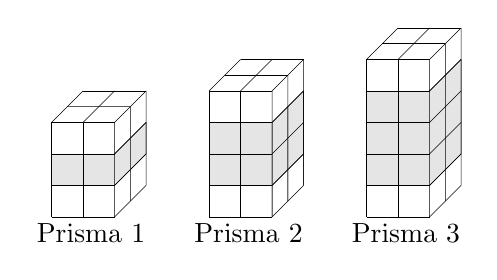
\begin{tikzpicture}[scale=2]
\fill[line width=2.pt,fill=black,fill opacity=0.10000000149011612] (0.,0.2) -- (0.400095,0.2) -- (0.6000712500000001,0.4) -- (0.6000475000000001,0.6) -- (0.4,0.4) -- (0.,0.4) -- cycle;
\draw[very thin] (0.,0.)-- (0.40019,0.);
\draw[very thin] (0.,0.4)-- (0.4,0.4);
\draw[very thin] (0.,0.6)-- (0.4,0.6);
\draw[very thin] (0.4,0.6)-- (0.6000237500000001,0.8);
\draw[very thin] (0.400095,0.2)-- (0.6000712500000001,0.4);
\draw[very thin] (0.4,0.4)-- (0.6000475000000001,0.6);
\draw[very thin] (0.400095,0.2)-- (0.,0.2);
\draw[very thin] (0.40019,0.)-- (0.600095,0.2);
\draw[very thin] (0.,0.6)-- (0.2,0.8);
\draw[very thin] (0.2,0.8)-- (0.6000237500000001,0.8);
\draw[very thin] (0.4,0.8)-- (0.2,0.6);
\draw[very thin] (0.1,0.7)-- (0.5000356207707869,0.7000237429513112);
\draw[very thin] (0.,0.)-- (0.,0.6);
\draw[very thin] (0.2,0.6)-- (0.2,0.);
\draw[very thin] (0.40019,0.)-- (0.4,0.6);
\draw[very thin] (0.6000237500000001,0.8)-- (0.600095,0.2);
\draw[very thin] (0.5001425,0.1)-- (0.5000356207707869,0.7000237429513112);
\draw[very thin] (0.,0.2)-- (0.400095,0.2);
\draw[very thin] (0.400095,0.2)-- (0.6000712500000001,0.4);
\draw[very thin] (0.6000712500000001,0.4)-- (0.6000475000000001,0.6);
\draw[very thin] (0.6000475000000001,0.6)-- (0.4,0.4);
\draw[very thin] (0.4,0.4)-- (0.,0.4);
\draw[very thin] (0.,0.4)-- (0.,0.2);
\draw(.25,-.1) node {Prisma 1};
\begin{scope}[xshift=1cm]
\fill[line width=2.pt,fill=black,fill opacity=0.10000000149011612] (0.,0.6) -- (0.,0.2) -- (0.400095,0.2) -- (0.6000712500000001,0.4) -- (0.6000237500000001,0.8) -- (0.4,0.6) -- cycle;
\draw[very thin] (0.600095,0.2)-- (0.6,1.);
\draw[very thin] (0.6,1.)-- (0.2,1.);
\draw[very thin] (0.,0.8)-- (0.,0.);
\draw[very thin] (0.,0.)-- (0.40019,0.);
\draw[very thin] (0.40019,0.)-- (0.4,0.8);
\draw[very thin] (0.4,0.8)-- (0.,0.8);
\draw[very thin] (0.,0.4)-- (0.4,0.4);
\draw[very thin] (0.2,0.8)-- (0.2,0.);
\draw[very thin] (0.,0.6)-- (0.4,0.6);
\draw[very thin] (0.4,0.6)-- (0.6000237500000001,0.8);
\draw[very thin] (0.5,0.9)-- (0.5001425,0.1);
\draw[very thin] (0.400095,0.2)-- (0.6000712500000001,0.4);
\draw[very thin] (0.4,0.4)-- (0.6000475000000001,0.6);
\draw[very thin] (0.400095,0.2)-- (0.,0.2);
\draw[very thin] (0.1,0.9)-- (0.5,0.9);
\draw[very thin] (0.2,0.8)-- (0.4,1.);
\draw[very thin] (0.40019,0.)-- (0.600095,0.2);
\draw[very thin] (0.4,0.8)-- (0.6,1.);
\draw[very thin] (0.,0.8)-- (0.2,1.);
\draw[very thin] (0.,0.)-- (0.,0.6);
\draw[very thin] (0.2,0.6)-- (0.2,0.);
\draw[very thin] (0.40019,0.)-- (0.4,0.6);
\draw[very thin] (0.6000237500000001,0.8)-- (0.600095,0.2);
\draw[very thin] (0.5001425,0.1)-- (0.5000356207707869,0.7000237429513112);
\draw[very thin] (0.,0.6)-- (0.,0.2);
\draw[very thin] (0.,0.2)-- (0.400095,0.2);
\draw[very thin] (0.400095,0.2)-- (0.6000712500000001,0.4);
\draw[very thin] (0.6000712500000001,0.4)-- (0.6000237500000001,0.8);
\draw[very thin] (0.6000237500000001,0.8)-- (0.4,0.6);
\draw[very thin] (0.4,0.6)-- (0.,0.6);
\draw(.25,-.1) node {Prisma 2};
\begin{scope}[xshift=1cm]
\fill[line width=2.pt,fill=black,fill opacity=0.10000000149011612] (0.,0.8) -- (0.4,0.8) -- (0.6,1.) -- (0.6000712500000001,0.4) -- (0.400095,0.2) -- (0.,0.2) -- cycle;
\draw[very thin] (0.,0.)-- (0.40019,0.);
\draw[very thin] (0.4,0.8)-- (0.,0.8);
\draw[very thin] (0.,0.4)-- (0.4,0.4);
\draw[very thin] (0.,0.6)-- (0.4,0.6);
\draw[very thin] (0.4,0.6)-- (0.6000237500000001,0.8);
\draw[very thin] (0.400095,0.2)-- (0.6000712500000001,0.4);
\draw[very thin] (0.4,0.4)-- (0.6000475000000001,0.6);
\draw[very thin] (0.400095,0.2)-- (0.,0.2);
\draw[very thin] (0.40019,0.)-- (0.600095,0.2);
\draw[very thin] (0.,1.)-- (0.2,1.2);
\draw[very thin] (0.,1.)-- (0.4,1.);
\draw[very thin] (0.4,1.)-- (0.6,1.2);
\draw[very thin] (0.2,1.)-- (0.4,1.2);
\draw[very thin] (0.2,1.2)-- (0.6,1.2);
\draw[very thin] (0.1,1.1)-- (0.5,1.1);
\draw[very thin] (0.,1.)-- (0.,0.);
\draw[very thin] (0.2,0.)-- (0.2,1.);
\draw[very thin] (0.4,1.)-- (0.40019,0.);
\draw[very thin] (0.5001425,0.1)-- (0.5,1.1);
\draw[very thin] (0.6,1.2)-- (0.600095,0.2);
\draw[very thin] (0.4,0.8)-- (0.6,1.);
\draw[very thin] (0.,0.8)-- (0.4,0.8);
\draw[very thin] (0.4,0.8)-- (0.6,1.);
\draw[very thin] (0.6,1.)-- (0.6000712500000001,0.4);
\draw[very thin] (0.6000712500000001,0.4)-- (0.400095,0.2);
\draw[very thin] (0.400095,0.2)-- (0.,0.2);
\draw[very thin] (0.,0.2)-- (0.,0.8);
\draw(.25,-.1) node{Prisma 3};
\end{scope}
\end{scope}
\end{tikzpicture}\end{figure}
\begin{enumerate}
\item {} 
Descreva, em palavras ou em linguagem simbólica, uma regra de formação sugerida pela figura.

\item {} 
Para construir o prisma \(4\) dessa sequência, segundo o padrão por você descrito, quantos cubos cinzas são necessários?

\item {} 
Justifique a afirmação: “O número total de cubos cinzas necessários para construir qualquer prisma desta sequência é par.”

\item {} 
Segundo o padrão por você descrito, quantos cubos cinzas terá o prisma 200?

\item {} 
Explicite uma expressão numérica que permita determinar o número de cubos cinzas do Prisma \(n\) em função de \(n\), isto é, uma expressão que de forma geral associe a ordem da figura à quantidade de cubos cinzas em sua composição.

\item {} 
Justifique novamente a afirmação do item (c), agora a partir da expressão que você explicitou no ítem anterior.

\item {} 
Se \(x\) representar o número total de cubos (brancos e cinzas) de um prisma desta sequência, qual das expressões seguintes representará o número de cubos cinzas desse prisma. Justifique sua escolha.

\end{enumerate}
\begin{equation*}
\begin{split}\square \ x-8 \quad \quad \square \ 2x-4 \quad \quad \square \ x-4 \quad \quad \square \ 4x\end{split}
\end{equation*}
\item  Ao final de um treino para a prova de 100 metros rasos, uma corredora recebe de seu treinador a seguinte tabela com as marcas intermediárias da sua melhor corrida.

\begin{table}[H]
\centering

\begin{tabu} to \textwidth{|c|c|}
\hline
\thead
Tempo (s) & Distância (m) \\
\hline
5 & $25$ \\
\hline
10 & $50$ \\
\hline
15 & $75$ \\
\hline
20 & $100$ \\
\hline
\end{tabu}
\end{table}

Considerando que a velocidade da atleta é constante ao longo dos 100 metros responda as seguintes perguntas.
\begin{enumerate}
\item {} 
Quanto tempo ela gastou para percorrer os primeiros \(30\) metros?

\item {} 
Pensando em uma estratégia para melhorar a preformance da atleta, seu treinador resolve detalhar a tabela com os tempos correspondentes a cada \(10\) metros. Construa essa tabela.

\end{enumerate}

\item Hoje de manhã a Ana saiu de casa e dirigiu-se para a escola. Fez uma parte do percurso andando e a outra parte correndo. O gráfico a seguir mostra a distância percorrida pela Ana, em função do tempo que decorreu desde o instante em que ela saiu de casa até ao instante em que chegou à escola.
\begin{center}\begin{tikzpicture}
\draw [->](0,0)--(6.5,0);
\draw (6.3,0) node[above]{tempo};
\draw[->](0,0)--(0,4);
\draw (0,4) node [right]{dist\^{a}ncia};
\draw(0,0)--(1.5,2.7)--(5.5,3.5);
\draw[dashed](1.5,0)--(1.5,2.7)--(0,2.7);
\draw[dashed](5.5,0)--(5.5,3.5)--(0,3.5);
\draw(1.5,-.3) node {$t_1$};
\draw(5.5,-.3) node {$t_2$};
\draw(-.3,2.7) node {$d_1$};
\draw(-.3,3.5) node {$d_1$};
\end{tikzpicture}\end{center}
Apresentam-se, a seguir, quatro afirmações. De acordo com o gráfico, apenas uma é verdadeira. Assinale-a com X, explicando por que motivo cada uma das demais opções é falsa.

( { } ) A Ana percorreu metade da distância andando e a outra metade correndo.

( { } ) A Ana percorreu maior distância andando do que correndo.

( { } ) A Ana esteve mais tempo correndo do que andando.

( { } ) A Ana iniciou o percurso correndo e terminou-o andando.

\item Em Janeiro, o Vitor, depois de ter vindo do barbeiro, decidiu estudar o comprimento do seu cabelo, registando todos os meses a sua medida. O gráfico seguinte representa o crescimento do cabelo do Vitor, desde o mês de Janeiro (mês 0), até ao mês de Junho (mês 5).
\phantomsection\label{\detokenize{AF106-E1:fig-cabelo}}

\begin{center}
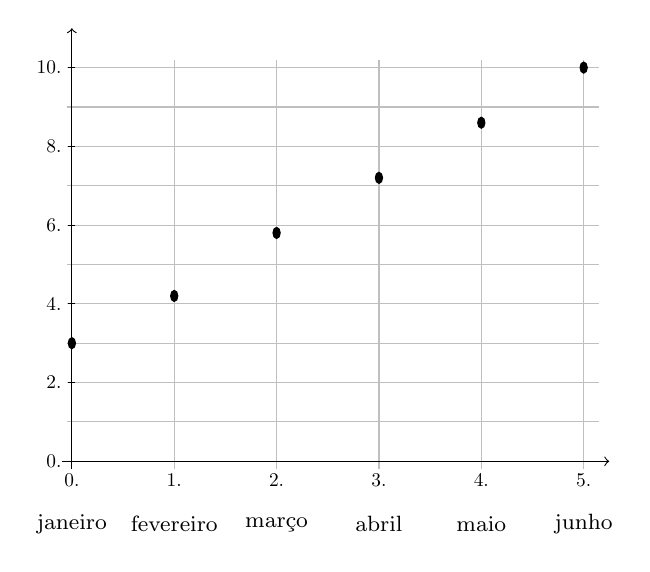
\begin{tikzpicture}[xscale=.65]
\draw [color=lightgray,, xstep=2.0cm,ystep=.5cm] (-.1,-.1) grid (10.3,5.1);
\draw[->,color=black] (-.2,0.) -- (10.5,0.);
\foreach \x in {0., 1.,2.,3.,4.,5.}
\draw[shift={(2*\x,0)},color=black] (0pt,-2pt) -- (0pt,-2pt) node[below, scale=.7] { $\x$};
\foreach \m[count=\x from 0]in {{janeiro} , {fevereiro} , {março}, {abril}, {maio}, {junho}}
\draw (2*\x, -.8) node {\footnotesize \m};
\draw[->,color=black] (0.,-.1) -- (0.,5.5);
\foreach \y in {0., 2.,4.,6., 8., 10.}
\draw[shift={(0,.5*\y)},color=black] (2pt,0pt) -- (-2pt,0pt) node[left, scale=.7] { $\y$};
\draw [fill](0,1.5) circle (2pt);
\draw [fill](2,2.1) circle (2pt);
\draw [fill](4,2.9) circle (2pt);
\draw [fill](6,3.6) circle (2pt);
\draw [fill](8,4.3) circle (2pt);
\draw [fill](10,5) circle (2pt);
\end{tikzpicture}\end{center}\begin{enumerate}
\item {} 
A partir dos dados apresentados no gráfico, complete a tabela acima.

\item {} 
Em cada mês, quantos centímetros cresceu o cabelo do Vitor?

\item {} 
Escreva uma expressão geral que represente o Comprimento (C) do cabelo do Vitor, em função do número de meses (M) passados após o corte de cabelo inicial.

\item {} 
Considerando o comportamento indicado no gráfico, se o cabelo do Vitor crescer \(19,8 \ cm\), se que haja cortes no período, quantos meses terão se passado desde o último corte de cabelo? Justifique.

\end{enumerate}

\item Considere a função \(g:\mathbb{R}\to\mathbb{R}\quad\) tal que \(\quad g(x)=9-x^2\).
\begin{enumerate}
\item {} 
Coloque em ordem crescente os números \(g(\sqrt{2})\), \(g(\sqrt{5})\) e  \(g(\sqrt{10})\).

\item {} 
Determine todos os possíveis valores de \(x\) do domínio que têm imagem igual a 8.

\item {} 
Existe algum \(x\in \mathbb{R}\) cuja imagem é igual a $10$? Por que?

\item {} 
Que condição deve satisfazer um número real \(b\) para que seja a imagem de algum número real \(x\), isto é, \(b=g(x)\) ?

\end{enumerate}

\item Considere o processo que associa \emph{cada número natural à soma de seus algarismos}.
\begin{enumerate}
\item {} 
Por meio do processo descrito acima o número natural \(13717\) será associado a que número?

\item {} 
Proponha um número cujo resultado do processo seja \(22\).

\item {} 
Quantos números entre \(1\) e \(10000\) nos levam ao resultado \(3\)?

\item {} 
É possível obter qualquer número natural como resultado desse processo? Explique.

\end{enumerate}
\end{enumerate}


\cleardoublepage
\def\currentcolor{session1}
\begin{objectives}{Ação promocional}
{
\begin{itemize}

\item Reconhecer vantagens da representação gráfica. Na questão, mais especificamente, em detrimento da representação na forma de tabela.

\item Argumentar a partir da análise de gráficos e/ou tabelas.

\end{itemize}
}{1}{1}
\end{objectives}
\begin{sugestions}{Ação promocional}
{
\begin{itemize}
\item Observe para os seus alunos que tabela e gráfico têm seus papéis. Ainda que um gráfico seja importante para um determinado objetivo, ele não exclui uso da tabela, que pode ser importante para outros objetivos. Uma tabela não substitui um gráfico se o domínio da função for um conjunto infinito, por exemplo.

\item Para os itens de análise do crescimento e decrescimento do valor dos dados numéricos da imagem em função da variação apresentada, pode ser útil conectar os pontos, formando uma linha poligonal. Contudo é importante destacar que os segmentos que conectam os pontos consecutivos não são pontos correspondentes da função, uma vez que o domínio dessa função é um conjunto discreto.

\item O item (e) está mais relacionado com o contexto do problema. Algumas possíveis justificativas para o crescimento seriam: início de veiculação de alguma propaganda em TV ou rádio, utilização da \textit{hashtag} por alguma celebridade (publipost) ou Blog famoso. Para o decrescimento pode-se pensar na ocorrência de algum fato de grande destaque na mídia, surgimento de algum \textit{meme}, evento negativo associado à empresa, dentre outros.

\item Explore o fato de ter-se aqui duas representações: para qual representação o aluno olhou, em cada um dos itens? Conclua apontando para o fato de que, muitas vezes, uma representação é mais “esclarecedora” que outra.
\end{itemize}
}{1}{1}
\end{sugestions}
\clearmargin
\begin{answer}{Ação promocional}
{
\begin{enumerate}

\item $6$ vezes.

\item No décimo segundo dia.

\item Do segundo ao sexto dia, do sétimo ao décimo segundo dia, do décimo quarto ao décimo sexto dia, entre o vigésimo e vigésimo primeiro dia e entre o vigésimo quarto e vigésimo sétimo dia.

\item Do primeiro para o segundo dia, do sexto para o sétimo dia, do décimo segundo ao décimo quarto dia, do décimo sexto ao vigésimo dia e entre o vigésimo primeiro ao vigésimo quarto dia.

\item Resposta variada.

\end{enumerate}
}{1}
\end{answer}
\clearmargin
\begin{objectives}{Do mapa para o gráfico}
{
\begin{itemize}

\item Estabelecer representação gráfica para pares ordenados com coordenada não numérica.

\item Estender o domínio da função para o conjunto dos números reais positivos, a partir de uma tabela.

\item Reconhecer diferentes representações gráficas para uma mesma função.

\end{itemize}
}{1}{1}
\end{objectives}
\begin{sugestions}{Do mapa para o gráfico}
{
\begin{itemize}
\item No item (a) espera-se que o estudante indique um conjunto de pares ordenados da forma: $\{(13, \text{Verde}),(15, \text{Laranja}),...\}$.

\item É natural que a primeira representação gráfica dos estudantes seja em um plano cartesiano, com as cores indicadas no eixo vertical. Essa é a resposta esperada para o item (b). No entanto, no último item, espera-se que sejam exploradas outras formas de representação, usando ou não eixos cartesianos. Uma representação possível é a partir de um retângulo colorido como a escala apresentada no item (a) da atividade "Colorindo o gráfico", em que se indique os tempos em que ocorre a mudança de cor, veja imagem na resposta da atividade.

\item Estimule a criatividade nas representações.

\item Caso algum estudante resolva simplesmente inverter os eixos, colocando as cores no eixo horizontal (como domínio), chame a atenção para o fato de que a relação inversa não é função.

\item No item (c) há várias respostas possíveis. Para que a resposta esteja correta, é necessário que todo o intervalo está coberto, ou seja, o domínio considerado é $[0,23]$. Além disso, não deve haver interseção entre os subintervalos.
\end{itemize}
}{0}{1}
\end{sugestions}
\begin{answer}{Do mapa para o gráfico}
{
\begin{enumerate}
\item Uma possibilidade é $\{(13,\text{verde}),(14,\text{verde}),(15,\text{laranja}),(18,\text{vermelha}),\\(23, \text{vinho})\}$

\item Três possíveis representações são:

\resizebox{.9\linewidth}{!}
{
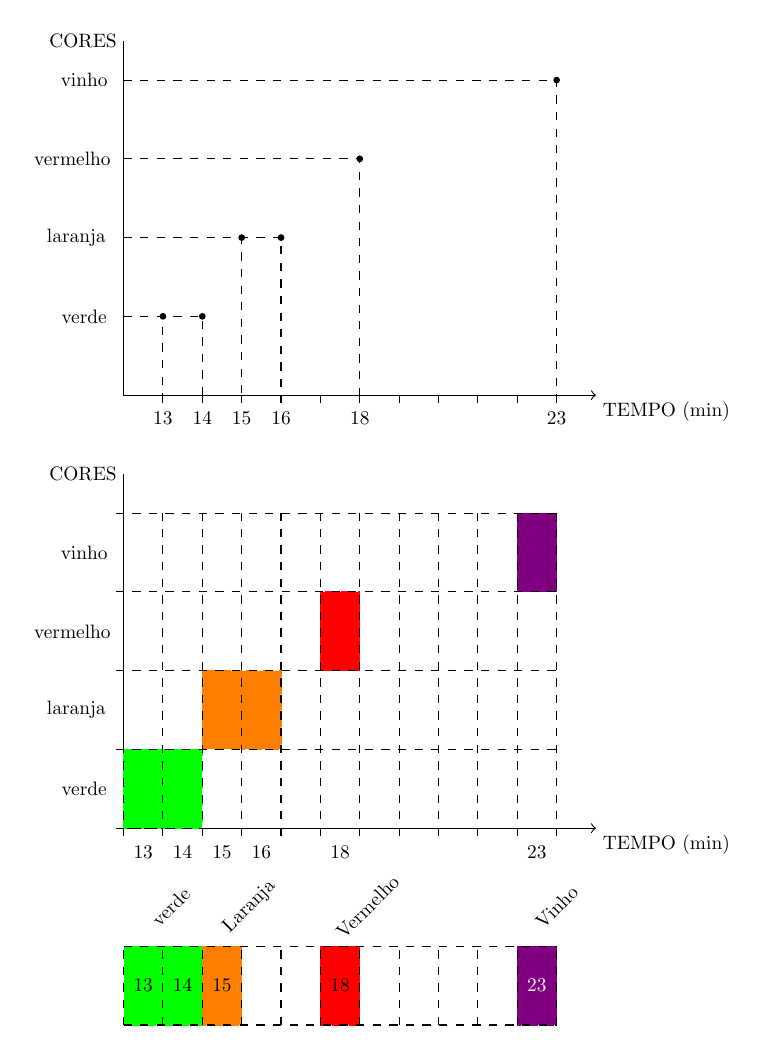
\begin{tikzpicture}
\draw[->](0,4.5) node[left, scale=.7]{CORES}--(0,0)--(6,0) node[below right, scale=.7]{TEMPO (min)};
\foreach \x in{1, 2, 3, 4, 5, 6, 7, 8, 9, 10, 11}
\draw(.5*\x, -.1)--(.5*\x,0);
\draw(.5,-.3) node[scale=.7]{13};
\draw(1,-.3) node[scale=.7]{14};
\draw(1.5,-.3) node[scale=.7]{15};
\draw(2,-.3) node[scale=.7]{16};
\draw(3,-.3) node[scale=.7]{18};
\draw(5.5,-.3) node[scale=.7]{23};
\draw(-.5,1)node[scale=.7]{verde};
\draw(-.6,2)node[scale=.7]{laranja};
\draw(-.65,3)node[scale=.7]{vermelho};
\draw(-.5,4)node[scale=.7]{vinho};
\draw[dashed](0,1)--(.5,1)--(.5,0);
\draw[dashed](0,1)--(1,1)--(1,0);
\draw[dashed](0,2)--(1.5,2)--(1.5,0);
\draw[dashed](0,2)--(2,2)--(2,0);
\draw[dashed](0,3)--(3,3)--(3,0);
\draw[dashed](0,4)--(5.5,4)--(5.5,0);
\draw[fill](.5,1)circle(1pt);
\draw[fill](1,1)circle(1pt);
\draw[fill](1.5,2)circle(1pt);
\draw[fill](2,2)circle(1pt);
\draw[fill](3,3)circle(1pt);
\draw[fill](5.5,4)circle(1pt);
\begin{scope}[yshift=-5.5cm]
\draw[->](0,4.5) node[left, scale=.7]{CORES}--(0,0)--(6,0) node[below right, scale=.7]{TEMPO (min)};
\foreach \x in{1, 2, 3, 4, 5, 6, 7, 8, 9, 10, 11}
\draw(.5*\x, -.1)--(.5*\x,0);
\draw(.25,-.3) node[scale=.7]{13};
\draw(.75,-.3) node[scale=.7]{14};
\draw(1.25,-.3) node[scale=.7]{15};
\draw(1.75,-.3) node[scale=.7]{16};
\draw(2.75,-.3) node[scale=.7]{18};
\draw(5.25,-.3) node[scale=.7]{23};
\draw(-.5,0.5)node[scale=.7]{verde};
\draw(-.6,1.5)node[scale=.7]{laranja};
\draw(-.65,2.5)node[scale=.7]{vermelho};
\draw(-.5,3.5)node[scale=.7]{vinho};
\draw[dashed,fill, color=green](0,0) rectangle (.5,1);
\draw[black,dashed,fill, color=green](.5,0) rectangle (1,1);
\draw[dashed,fill, color=orange](1,1) rectangle (1.5,2);
\draw[black,dashed,fill, color=orange](1.5,1) rectangle (2,2);
\draw[black,dashed,fill, color=red](2.5,2) rectangle (3,3);
\draw[black,dashed,fill, color=violet](5,3) rectangle (5.5,4);
\draw [color=black,dashed, xstep=.5cm,ystep=1cm] (-.1,-.1) grid (5.5,4);
\begin{scope}[yshift=-2.5cm]
\draw[dashed,fill, color=green](0,0) rectangle (1,1);
\draw[dashed,fill, color=orange](1,0) rectangle (1.5,1);
\draw[dashed,fill, color=red](2.5,0) rectangle (3,1);
\draw[black,dashed,fill, color=violet](5,0) rectangle (5.5,1);
\draw (.6,1.5)node[scale=.7, rotate=45]  {verde};
\draw (.25,.5)node[scale=.7]  {13};
\draw (.75,.5)node[scale=.7]  {14};
\draw(1.25,.5) node[scale=.7]{15};
\draw(2.75,.5) node[scale=.7]{18};
\draw[white](5.25,.5) node[scale=.7]{23};
\draw (1.6,1.5)node[scale=.7, rotate=45]  {Laranja};
\draw (3.1,1.5)node[scale=.7, rotate=45]  {Vermelho};
\draw (5.5,1.5)node[scale=.7, rotate=45]  {Vinho};
\draw [color=black,dashed, xstep=.5cm,ystep=1cm] (0,0) grid (5.5,1);
\end{scope}\end{scope}
\end{tikzpicture}
}

\item Uma possibilidade de reposta é: verde para $t\in [0,15[$, laranjar para $t\in[15,18[$, vermelho para $t\in[18,23[$ e vinho para $t\in[25,25]$

\item Ver item (b)

\end{enumerate}
}{0}
\end{answer}
\begin{objectives}{Números triangulares no plano}
{
\begin{itemize}

\item Representar graficamente.

\end{itemize}
}{1}{1}
\end{objectives}
\begin{sugestions}{Números triangulares no plano}
{
\begin{itemize}
\item Destaque para os seus alunos que nesse caso não cabe ligar os pontos. As abscissas indicam a ordem sequencial dos números triangulares, portanto, resumem-se apenas a números naturais.

\item Observe que os pontos do gráfico não são colineares.
\end{itemize}
}{1}{1}
\end{sugestions}
\begin{answer}{Números triangulares no plano}
{
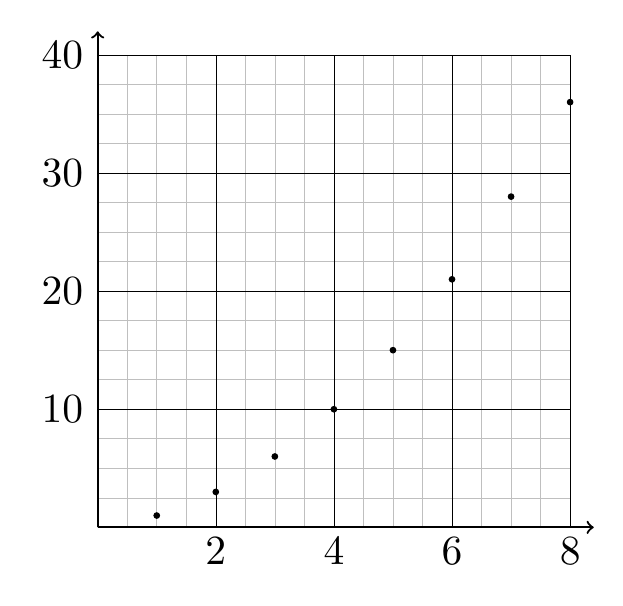
\begin{tikzpicture}[scale=1.5, every node/.style={scale=1.5, black}, every path/.style={color=black}]

\tikzstyle{ponto}=[circle, minimum size=2pt, inner sep=0, draw=black, fill=black, shift only]
\draw[help lines,xstep=.25,ystep=.25, lightgray] (0,0) grid (4,4);
\draw[help lines, black, xstep=1, ystep=1] (0,0) grid (4,4);
\draw[thick,->](0,0)--(4.2,0);
\draw[thick,->](0,0)--(0,4.2);
\foreach \x in {2, 4, 6, 8}
\draw(.5*\x,-.2)node{\x};
\foreach \x in{1, 2, 3, 4, 5, 6, 7, 8}
\node[ponto] at(.5*\x, {.05*\x*(1+\x)}){};
\foreach \y in{10, 20, 30, 40}
\draw(0,.1*\y) node[left]{\y};

\end{tikzpicture}
}{0}
\end{answer}
\clearmargin
\begin{objectives}{Jornada até a escola}
{
\begin{itemize}

\item  Representar pontos no plano cartesiano a partir de uma situação real.

\item  Estabelecer uma função a partir da seleção de pontos em um sistema cartesiano, associando a univocidade à identificação de apenas um ponto para cada valor da abscissa.

\end{itemize}
}{1}{2}
\end{objectives}
\begin{sugestions}{Jornada até a escola}
{
\begin{itemize}
\item Durante a discussão, chame a atenção para a necessidade de certificar-se da associação de um único valor de ordenada para cada valor de abscissa.

\item Discuta com os estudantes sobre o significado dos segmentos de reta que conectam os pontos.
\end{itemize}
}{1}{2}
\end{sugestions}
\begin{answer}{Jornada até a escola}
{
\begin{enumerate}

\item A jornada de Leonardo é descrita pelo gráfico abaixo:

\begin{tikzpicture}

\tikzstyle{ponto}=[circle, minimum size=2pt, inner sep=0, draw=black, fill=black, shift only]
\begin{scope}[yscale=.7, every node/.style={black}, every path/.style={black}]
\draw[help lines,xstep=.2,ystep=.25, lightgray] (0,0) grid (6.5,6.2);
\draw[help lines, black, xstep=1, ystep=1] (0,0) grid (6.5,6.2);
\draw[thick,->](-.6,0)--(6.5,0) node[below left, yshift =-.2cm]{\tiny tempo(minutos)};
\draw[thick,->](0,-.4)--(0,6.2) node[rotate=90,left,yshift =.7cm]{\tiny distância percorrida (km)};
\foreach \x in {5, 10, ..., 30}
\draw(.2*\x,-.3)node{\x};
\foreach \y in {1, 2, 3, 4, 5, 6}
\draw(-.3, \y)node{\y};
\node[ponto] at(0,0){};\node[ponto] at(0,1){};\node[ponto] at(1,.2){};\node[ponto] at(1,.51){};\node[ponto] at(1,1.2){};\node[ponto] at(1,2){};\node[ponto] at(2,0){};\node[ponto] at(2,0.9){};\node[ponto] at(2,1.4){};\node[ponto] at(2,1.6){};\node[ponto] at(2,3){};\node[ponto] at(3,1.2){};\node[ponto] at(3,2.5){};\node[ponto] at(3,1.4){};\node[ponto] at(3,2){};\node[ponto] at(3,4){};\node[ponto] at(4,1.6){};\node[ponto] at(4,2.7){};\node[ponto] at(4,2.9){};\node[ponto] at(4,3.2){};\node[ponto] at(4,4){};\node[ponto] at(5,2){};\node[ponto] at(5,3.2){};\node[ponto] at(5,4){};\node[ponto] at(5,5){};\node[ponto] at(5,6){};\node[ponto] at(6,2.5){};\node[ponto] at(6,4){};\node[ponto] at(6,5){};\node[ponto] at(6,5.8){};\node[ponto] at(6,6){};
\draw[thick, session3](0,0)--(1,0)--(2,3)--(3,4)--(4,4)--(5,6)--(6,6);
\end{scope}
\end{tikzpicture}


\item Aproximadamente $1{,}25$ km

\item Resposta pessoal.

\end{enumerate}
}{1}
\end{answer}

\explore{Gráficos}
Segundo informações do \href{http://www.bigdatabusiness.com.br/visualizacao-de-dados-por-que-transformar-big-data-em-graficos/}{Big Data Business}, as palavras estimulam o lado esquerdo do cérebro e são um recurso essencial para a manutenção da memória. No entanto, as imagens são ainda mais eficazes, porque elas conseguem ativar os dois lados do cérebro simultaneamente e, assim, permitem o resgate de ideias e informações com maior precisão e agilidade. Especialmente quando se quer analisar grande quantidade de dados, apresentá-los em uma imagem ou em um gráfico, pode favorecer a comunicação.

\begin{figure}[H]
\centering
\capstart

\noindent\includegraphics[width=400bp]{{grafico-final}.png}
\caption{Alguns exemplos de representações gráficas}\label{\detokenize{AF106-4:id1}}\end{figure}

Representar graficamente conjuntos de dados e suas relações pode fazer toda a diferença para transmitir informações. Há vários tipos de gráficos, cada um tem a sua particularidade e serve para transmitir as informações de forma específica. Nesta seção iremos estudar a representação gráfica de funções.

Vamos considerar a seguinte situação:


\begin{task}{ ação promocional}
\label{\detokenize{AF106-4:atividade-acao-promocional}}

Uma empresa resolve lançar uma ação promocional na internet usando uma \href{https://pt.wikipedia.org/wiki/Hashtag}{hashtag}. Um mês após o lançamento, o presidente dessa empresa resolve analisar o impacto da ação na rede. Para isso ele pede a um de seus funcionários que prepare um relatório sobre o número de vezes que a \emph{hashtag} foi mencionada nas redes sociais em cada dia durante aquele mês. O funcionário resolveu apresentar os dados das seguintes duas formas:
\begin{figure}[H]
\centering

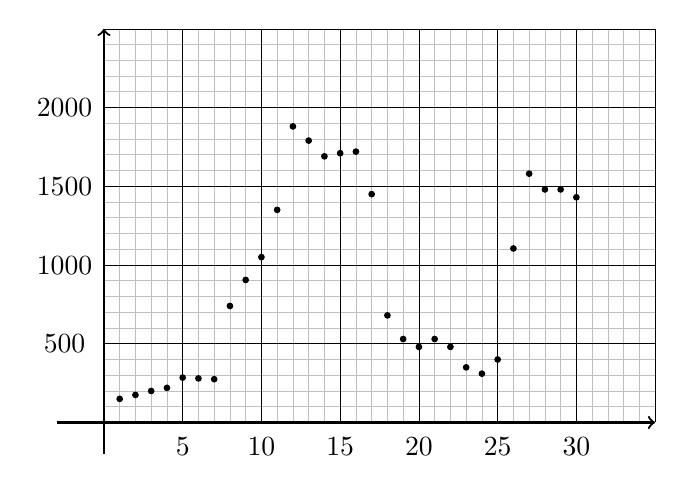
\begin{tikzpicture}
\tikzstyle{ponto}=[circle, minimum size=2pt, inner sep=0, draw=black, fill=black, shift only]
\draw[help lines,xstep=.2,ystep=.2, lightgray] (0,0) grid (7,5);
\draw[help lines, black, xstep=1, ystep=1] (0,0) grid (7,5);
\draw[thick,->](-.6,0)--(7,0);
\draw[thick,->](0,-.4)--(0,5);
\foreach \x in {5, 10, ..., 30}
\draw(.2*\x,-.3)node{\x};
\foreach \y in {500, 1000, 1500, 2000}
\draw(-.5, .002*\y)node{\y};
\node [ponto] at (.2,.3){};
\node [ponto] at (.4,.35){};\node [ponto] at (.6,.4){};\node [ponto] at (.8,.44){};   \node [ponto] at (1,.57){};\node [ponto] at (1.2,.56){};\node [ponto] at (1.4,.55){};\node [ponto] at (1.6,1.48){};\node [ponto] at (1.8,1.81){};\node [ponto] at (2,2.1){};\node [ponto] at (2.2,2.7){};\node [ponto] at (2.4,3.76){};\node [ponto] at (2.6,3.58){};\node [ponto] at (2.8,3.38){};\node [ponto] at (3,3.42){};\node [ponto] at (3.2,3.44){};\node [ponto] at (3.4,2.9){};\node [ponto] at (3.6,1.36){};\node [ponto] at (3.8,1.06){};\node [ponto] at (4,.96){};\node [ponto] at (4.2,1.06){};\node [ponto] at (4.4,.96){};\node [ponto] at (4.6,.7){};\node [ponto] at (4.8,.62){};\node [ponto] at (5.,.8){};\node [ponto] at (5.2,2.21){};\node [ponto] at (5.4,3.16){};\node [ponto] at (5.6,2.96){};;  \node [ponto] at (5.8,2.96){};;\node [ponto] at (6,2.86){};
\end{tikzpicture}
\end{figure}
\begin{enumerate}
\item {} 
Quantas vezes a \emph{hashtag} foi mencionada mais de 1500 vezes em um dia?

\item {} 
Em que dia a \emph{hashtag} foi mais citada?

\item {} 
Identifique todos os períodos em que houve crescimento no número de citações.

\item {} 
Faça o mesmo para o decrescimento.

\item {} 
Escreva um parágrafo explicando o comportamento global do gráfico, apontando possíveis causas para as variações observadas.

\end{enumerate}

\end{task}

Uma função, essencialmente, relaciona duas ou mais grandezas ou variáveis, de forma que são obtidos pares \((x,y)\), em que \(x\) pertence ao domínio da função e \(y=f(x)\). Perceba que a ordem em que os termos que compõem o par são apresentados é importante. Em matemática, chamamos esse tipo de objeto de \emph{par ordenado}, eles são objetos fundamentais para a compreensão do gráfico de uma função.

No caso de funções reais de variável real, isto é, cujos domínio e contradomínio são o conjunto dos números reais (ou subconjuntos dele) tanto \(x\) como \(y\) serão números reais.

A representação geométrica mais comum para esses pontos, e que você provavelmente já conhece, é no \index{plano cartesiano}plano cartesiano. Essa representação tem como base duas retas numéricas perpendiculares que se intersectam em suas origens conforme a figura abaixo.

\begin{center}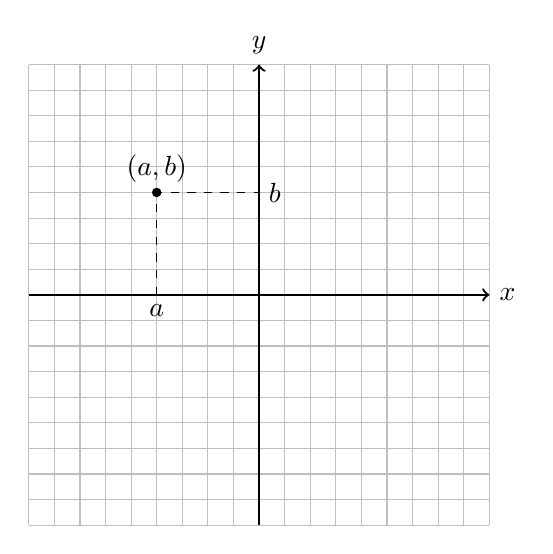
\begin{tikzpicture}[scale=.65]
\tikzstyle{ponto}=[circle, minimum size=3pt, inner sep=0, draw=black, fill=black, shift only]
\draw[lightgray](-4.5,-4.5)grid[xstep=.5,ystep=.5,line width =1pt](4.5,4.5);
\draw[->,thick](-4.5,0)--(4.5,0) node[right]{$x$};
\draw[->,thick](0,-4.5)--(0,4.5)node[above]{$y$};
\draw[dashed](-2,0)--(-2,2)--(0,2);
\node[ponto] at (-2,2){};
\node[above] at (-2,2){$(a,b)$};
\node[below] at (-2,0){$a$};
\node[right] at (0,2){$b$};
\end{tikzpicture}\end{center}

As retas que compõem um sistema cartesiano são chamadas de \index{eixos coordenados}eixos do plano cartesiano. O eixo em que são registradas as primeiras coordenadas do par é chamado de \index{eixo das abscissas}eixo das abscissas. O outro eixo, em que são registradas as segundas coordenadas do par é chamado de \index{eixo das ordenadas}eixo das ordenadas.

Já vimos alguns exemplos de funções em atividades anteriores, vamos explorá-los um pouco mais.


\begin{task}{ do mapa para o gráfico}
\label{\detokenize{AF106-4:ativ-funcoes-do-mapa-para-grafico}}\label{\detokenize{AF106-4:atividade-do-mapa-para-o-grafico}}

\begin{enumerate}
\item {} 
A partir das colunas \emph{Tempo de travessia} e \emph{Cor} da {\hyperref[\detokenize{AF106-2:ativ-funcoes-colorindo-o-mapa}]{Atividade: colorindo o mapa}}, escreva o conjunto de pares ordenados da forma (tempo, cor) respeitando o critério que você escolheu para a determinação das cores.

\item {} 
Represente graficamente este conjunto de pares ordenados.

\item {} 
Para colorir as vias de todo o mapa, precisamos distribuir as cores para outros valores de tempo. Como você faria a distribuição para o intervalo de \(0\) a \(25\) minutos considerando um trecho qualquer de \(13\) km (a mesma extensão da ponte)?

\item {} 
Encontre outra maneira de representar graficamente a associação entre os tempos e as cores.

\end{enumerate}

\end{task}

\begin{task}{ números triangulares no plano}
\label{\detokenize{AF106-4:atividade-numeros-triangulares-no-plano}}\label{\detokenize{AF106-4:ativ-funcoes-numeros-triangulares}}

Represente, no plano cartesiano, o conjunto de pontos que correspondem aos pares ordenados \(\{(n,T_n)\ ;\ n\in\{1,2,...,8\}\}\), em que \(T_n\) é o \(n\)-ésimo número triangular.

\end{task}

\begin{task}{ jornada até a escola}
\label{\detokenize{AF106-4:atividade-jornada-ate-a-escola}}\label{\detokenize{AF106-4:ativ-funcoes-jornada-ate-a-escola}}

Leonardo mora a \(6\) km da escola onde estuda e utiliza o transporte escolar, que o busca na porta de sua casa. Em um certo dia, o percurso de Leonardo até sua escola foi assim: Ele estava na porta de casa às \(7\) horas, como de costume, mas o transporte escolar atrasou, passando em sua casa somente às \(7h05min\). Leonardo entrou na van e sentou no penúltimo lugar vago. Ainda faltava Marina. “Ela mora a \(3\) km da minha casa!”, lembrou Leonardo. Às \(7h10min\) em ponto, o transporte escolar chegou à casa de Marina, que já estava pronta aguardando para embarcar. Para tentar compensar o atraso, o motorista resolveu tomar um atalho, mas a estratégia não funcionou. Às \(7h15min\) precisou ficar parado por \(5\) minutos em frente a uma cancela aguardando um trem de carga passar. Finalmente, às \(7h25min\) chegaram à escola, \(5\) minutos antes do sinal tocar.

No plano cartesiano a seguir, o eixo horizontal indica o tempo em minutos e o eixo vertical a distância percorrida em quilômetros. Os pontos marcados correspondem às distâncias percorridas por diversos estudantes da escola a cada \(5\) minutos no período das \(7h\) às \(7h30min\) da mesma manhã descrita na situação acima.

\phantomsection\label{\detokenize{AF106-4:fig-pontos-jornada}}
\begin{figure}[H]
\centering

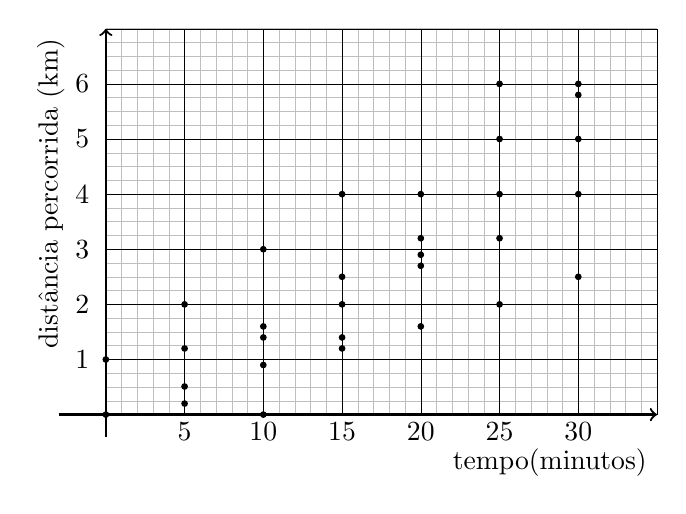
\begin{tikzpicture}
\tikzstyle{ponto}=[circle, minimum size=2pt, inner sep=0, draw=black, fill=black, shift only]
\begin{scope}[yscale=.7]
\draw[help lines,xstep=.2,ystep=.25, lightgray] (0,0) grid (7,7);
\draw[help lines, black, xstep=1, ystep=1] (0,0) grid (7,7);
\draw[thick,->](-.6,0)--(7,0) node[below left, yshift =-.3cm]{tempo(minutos)};
\draw[thick,->](0,-.4)--(0,7) node[rotate=90,left,yshift =.7cm]{ distância percorrida (km)};
\foreach \x in {5, 10, ..., 30}
\draw(.2*\x,-.3)node{\x};
\foreach \y in {1, 2, 3, 4, 5, 6}
\draw(-.3, \y)node{\y};
\node[ponto] at(0,0){};\node[ponto] at(0,1){};\node[ponto] at(1,.2){};\node[ponto] at(1,.51){};\node[ponto] at(1,1.2){};\node[ponto] at(1,2){};\node[ponto] at(2,0){};\node[ponto] at(2,0.9){};\node[ponto] at(2,1.4){};\node[ponto] at(2,1.6){};\node[ponto] at(2,3){};\node[ponto] at(3,1.2){};\node[ponto] at(3,2.5){};\node[ponto] at(3,1.4){};\node[ponto] at(3,2){};\node[ponto] at(3,4){};\node[ponto] at(4,1.6){};\node[ponto] at(4,2.7){};\node[ponto] at(4,2.9){};\node[ponto] at(4,3.2){};\node[ponto] at(4,4){};\node[ponto] at(5,2){};\node[ponto] at(5,3.2){};\node[ponto] at(5,4){};\node[ponto] at(5,5){};\node[ponto] at(5,6){};\node[ponto] at(6,2.5){};\node[ponto] at(6,4){}; \node[ponto] at(6,5){};\node[ponto] at(6,5.8){};\node[ponto] at(6,6){};
\end{scope}
\end{tikzpicture}
\end{figure}


\begin{enumerate}
\item {} 
Conecte os pontos que correspondem à jornada de Leonardo, desde a porta da sua casa até a chegada à escola, no dia descrito acima.

\item {} 
Faça uma estimativa da distância a que Leonardo estará de sua casa às \(7h07min\).

\item {} 
Escolha um conjunto de pontos que possa representar a jornada de um outro estudante da sua casa à escola e descreva essa jornada.

\end{enumerate}
\end{task}

\arrange{Gráficos}
\label{\detokenize{AF106-5:sec-organizando-graficos}}\label{\detokenize{AF106-5:organizando-as-ideias-graficos}}\label{\detokenize{AF106-5::doc}}
É hora de organizar as ideias sobre representação gráfica de uma função. Vimos que, para representar graficamente as funções, os pares ordenados são fundamentais. Cada par identifica as grandezas ou variáveis relacionadas e a ordem no par distingue o papel de cada uma delas: elemento do domínio, abscissa, e imagem, ordenada. Sendo assim, a representação gráfica de uma função exige: a identificação das variáveis do problema e a identificação da relação estabelecida entre as variáveis.

Para funções reais de variável real, isto é, funções cujo domínio é um subconjunto de \(\mathbb{R}\) e o contradomínio é \(\mathbb{R}\), sua representação gráfica no plano cartesiano será o conjunto dos pares ordenados \((x,f(x))\) em que \(x\) pertence ao domínio da função.

\begin{figure}[H]
\centering

\begin{tikzpicture}[scale=1.5]
\draw[line width=1.pt,color=\currentcolor!80,samples=100,domain=-2.05:1.8] plot(\x,{.5*sin((3.5*(\x)-3.2)*180/pi)-0.6*cos((4.5*(\x)+2.0)*180/pi)});
\draw[->](-.8,-1)--(-.8,1.5) ;
\draw[->](-2.3,0)--(2.5,0);
\draw[fill](.965,-.5)circle(1pt);
\draw[dashed](-.8,-.5)--(.965,-.5);
\draw[dashed](.965,-.5)--(.965,-0);
\draw(.965,-0)node[scale=.5, above]{$x$};
\draw[dashed](-.8,-.5)node[left]{$f(x)$};
\draw(.97,-.55) node[right] {($x, f(x)$)};
\end{tikzpicture}
\end{figure}

\begin{reflection}

Os conjuntos domínio e imagem ficam evidenciados na representação gráfica de uma  função a partir dos eixos coordenados. Observe a representação gráfica a seguir, em que estão destacados conjuntos sobre os eixos. Qual deles você identifica como domínio? A que conjunto corresponde o outro?
\begin{figure}[H]
\centering

\begin{tikzpicture}[scale=1.5]
\draw[line width=1.pt,color=\currentcolor!80,samples=100,domain=-1.5:1.8] plot(\x,{.5*sin((3.5*(\x)-3.2)*180/pi)-0.6*cos((4.5*(\x)+2.0)*180/pi)});
\draw[->](-.8,-1)--(-.8,2) ;
\draw[->](-2,0)--(2.5,0);
\draw[dashed](-2,.95)--(2.5,.95);
\draw[dashed](-2,-.67)--(2.5,-.67);
\draw[color=red, thick](-.8, -.67)--(-.8, .95);
\begin{scope}[xshift=5cm]
\draw[line width=1.pt,color=\currentcolor!80,samples=100,domain=-1.5:1.8] plot(\x,{.5*sin((3.5*(\x)-3.2)*180/pi)-0.6*cos((4.5*(\x)+2.0)*180/pi)});
\draw[->](-.8,-1)--(-.8,2) ;
\draw[->](-2,0)--(2.5,0);
\draw[dashed](-1.5,-1)--(-1.5,2);
\draw[dashed](1.8,-1)--(1.8,2);
\draw[color=blue, thick](-1.5,0)--(1.8,0);
\end{scope}
\end{tikzpicture}\
\end{figure}
\end{reflection}

\clearpage

\def\currentcolor{session2}
\begin{objectives}{Indo para escola}
{
\begin{itemize}

\item Fazer uso de simbologia matemática para representar informações apresentadas pictórica e verbalmente.

\item Interpretar e relacionar informações a partir da representação gráfica apresentada.

\end{itemize}
}{1}{2}
\end{objectives}
\begin{sugestions}{Indo para escola}
{
\begin{itemize}
\item É importante que os estudantes percebam o significado de dois pontos estarem na mesma horizontal ou na mesma vertical.

\item Chame a atenção para o uso da escala.
\end{itemize}
}{1}{2}
\end{sugestions}
\begin{answer}{Indo para escola}
{
\begin{enumerate}

\item\adjustbox{valign=t}{\begin{minipage}{\linewidth}
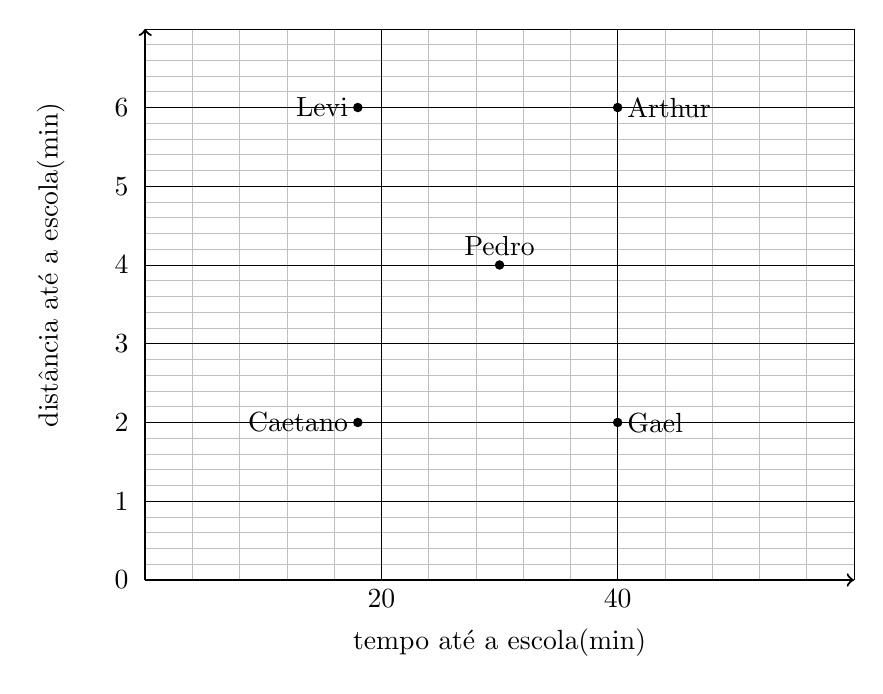
\begin{tikzpicture}
\tikzstyle{ponto}=[circle, minimum size=3pt, inner sep=0, draw=black, fill=black, shift only]
\begin{scope}[xscale=3, every node/.style={black}, every path/.style={black}]
\draw[help lines,xstep=.2,ystep=.2, lightgray] (0,0) grid (3,7);
\draw[help lines, black, xstep=1, ystep=1] (0,0) grid (3,7);
\draw[thick,->](0,0)--(3,0);
\draw[thick,->](0,0)--(0,7);
\draw(1.5,-.8)node{tempo até a escola(min)};
\draw(-.4,4)node[rotate=90]{distância até a escola(min)};
\node[ponto] at(.9,2){};
\node[ponto] at(.9,6){};
\node[ponto] at(1.5,4){};
\node[ponto] at(2,2){};
\node[ponto] at(2,6){};
\node[  left] at(.9,2){Caetano};
\node[left] at(.9,6){ Levi};
\node[above] at(1.5,4){Pedro};
\node[right] at(2,2){Gael};
\node[right] at(2,6){Arthur};
\foreach \y in{0,1, 2, 3, 4, 5, 6}
\draw(-.1,\y)node{\y};
\draw(1,0)node[below]{20};
\draw(2,0)node[below]{40};
\end{scope}
\end{tikzpicture}
\end{minipage}}

\item Pedro e Caetano foram para a escola de bicicleta ou correndo (ou de alguma forma que seja mais rápida do que ir a pé e mais lenta que ir de carro). Caetano e Gael moram ambos a $2$ km doa escola. Como Gael, que foi caminhando, levou $40$ minutos, Caetano que gastou aproximadamente $18$ minutos não pode ter ido caminhando. Caetano também não pode ter ido de carro, pois Levi que mora a $6$ km da escola demorou o mesmo tempo que ele e foi de carro.

\end{enumerate}
}{1}
\end{answer}
\clearmargin
\begin{objectives}{Qual é o gráfico?}
{
\begin{itemize}

\item  Reconhecer comportamentos crescente e decrescente em funções a partir de sua representação gráfica.


\item O “Para refletir”{} apresentado adiante, explora diferentes tipos de gráficos de funções decrescente e crescente. Procure fazer conexão desta atividade com esse “para Refletir”

\end{itemize}
}{1}{1}
\end{objectives}
\begin{sugestions}{Qual é o gráfico?}
{
\begin{itemize}
\item Fazer a conexão com o “Para refletir”{} apresentado mais adiante, onde são explorados diferentes tipos de gráficos de função decrescente e crescente.

\item Como os gráficos são apenas esboços, mais importante que os valores da tabela são as suas variações.
\end{itemize}
}{1}{1}
\end{sugestions}
\begin{answer}{Qual é o gráfico?}
{
\begin{enumerate}
\item (g)

\item (a)

\item (e) 

\item (k)

\end{enumerate}
}{1}
\end{answer}
\clearmargin
\begin{objectives}{Imaginando gráficos}
{
\begin{enumerate}

\item Reconhecer o comportamento crescente e decrescente de funções a partir de suas representações dadas. Sugere-se, associar esse comportamento a situações cotidianas.

\end{enumerate}
}{1}{2}
\end{objectives}
\begin{sugestions}{Imaginando gráficos}
{
\begin{itemize}
\item Não existe resposta única para cada item. Certifique-se de que seus estudantes tenham argumentos consistentes sobre as suas escolhas. Você pode sugerir que eles compartilhem entre si os seus argumentos.

\item É fundamental definir o que representa cada eixo, por exemplo, no item (I), se consideramos o tempo no eixo horizontal e a intensidade sonora no vertical, somente os gráficos (e) e (h) consideram o silêncio inicial, no entanto o gráfico (h) não leva em conta que “\textit{rapidamente} todos estavam aplaudindo e se manifestando”{} e ainda há diminuição na intensidade sonora. Portanto, o gráfico (e) é o mais adequado. Agora, caso coloquemos no eixo horizontal a quantidade pessoas aplaudindo, os mais adequados são os gráficos (a) ou (d), eles passam pela origem e são crescentes.
\end{itemize}
}{1}{2}
\end{sugestions}
\begin{answer}{Imaginando gráficos}
{
\begin{enumerate}[label=($\Roman*$)]
\item (e) eixo horizontal, eixo vertical: intensidade sonora.

\item (h) eixo horizontal: número de clientes, eixo vertical: lucro.

\item (k) eixo horizontal: tempo, eixo vertical: preço
\end{enumerate}
}{1}
\end{answer}
\clearmargin
\begin{objectives}{Para refletir}
{
  Aqui deseja-se que os alunos percebam que as funções que correspondem às representações gráficas da primeira linha são crescentes e as que correspondem às da segunda linha são decrescentes. Quanto às colunas, espera-se que tenham alguma ideia sobre a taxa de variação do crescimento (segunda derivada da função). Os da primeira coluna tem crescimento/decrescimento constante, os da segunda coluna, o crescimento/decrescimento é cada vez maior enquanto nos da terceira coluna é cada vez menor.
}{1}{1}
\end{objectives}

\clearmargin
\begin{objectives}{Leia no gráfico!}
{
\begin{itemize}

\item  Calcular, a partir da representação gráfica de uma função real de variável real, os valores de $f(x)$ e $x$ solicitados.

\end{itemize}
}{1}{2}
\end{objectives}
\begin{sugestions}{Leia no gráfico!}
{
\begin{itemize}
\item Todos os valores solicitados são exatos, esta opção foi feita com o intuito de facilitar a feitura da atividade. Caso julgue adequado você poderá explorar a determinação de valores aproximados, como por exemplo: $f(0,5)$ ou os valores aproximados de $x$ tais que $f(x)=0$.
\end{itemize}
}{1}{2}
\end{sugestions}
\begin{answer}{Leia no gráfico!}
{
\begin{table}[H]
\centering
\begin{tabu} to \textwidth{|l|>{$}c<{$}|}
\hline
\cellcolor{\currentcolor!80}\textcolor{white}{\textbf{Notação}} & \cellcolor{\currentcolor!80}\textcolor{white}{\textbf{Valor}} \\
\hline
\(f(1)-f(0)\) & 3 \\
\hline
\(4\cdot f(3)\) & 12 \\
\hline
\(f(4)/f(2)\) & 1/3 \\
\hline
\(f(6)\cdot f(2)\) & -6 \\
\hline
\(x\) quando \(f(x)=-2\) & x=6 \\
\hline
\(x\) quando \(f(x)=0\) & x=8 \\
\hline
\(f(3\cdot 2)-4\cdot f(\sqrt{81})+1\) & -21 \\
\hline
\end{tabu}
\end{table}
}{1}
\end{answer}
\clearmargin
\begin{objectives}{Imposto de renda}
{
\begin{itemize}

\item  Calcular imagens por uma função definida por mais de uma sentença

\item Transitar entre diferentes representações de função: tabela, expressão e gráfico

\end{itemize}
}{1}{1}
\end{objectives}
\begin{sugestions}{Imposto de renda}
{
\begin{itemize}
\item É bastante comum os estudantes acharem que se trata de várias funções em vez de uma única função definida por mais de uma sentença. Isso se dá pelo fato de fazerem confusão entre o conceito de função e a expressão que a define.
\end{itemize}
}{1}{1}
\end{sugestions}
\clearmargin
\begin{answer}{Imposto de renda}
{
\begin{enumerate}
\item Os valores são

\begin{enumerate}
\item R\$ $0$ 
\item R\$ $58{,}20$
\item R\$ $277{,}37$
\item R\$ $643{,}14$
\end{enumerate}

\item
\adjustbox{valign=t}{
\centering
\begin{tabu} to \textwidth{|c|c|c|}
\hline
\thead
Ponto & Alíquota & Salário \\
\hline
A & $7{,}5\%$ (segundo intervalo) & R\$ $2600{,}00$\\
\hline
B & $15\%$ (terceiro intervalo) & R\$ $3400{,}00$\\
\hline
C & $22{,}5\%$ (quarto intervalo) & R\$ $4000{,}00$\\ 
\hline
\end{tabu}}

\end{enumerate}
}{1}
\end{answer}
\clearmargin
\begin{objectives}{Planos telefônicos}
{
\begin{itemize}

\item Interpretar informações registradas textual e graficamente.

\item Visualizar o gráfico de uma função definida por mais de uma sentença.

\item  Utilizar informações de um gráfico para tomada de decisão.

\end{itemize}
}{1}{1}
\end{objectives}
\begin{sugestions}{Planos telefônicos}
{
\begin{itemize}
\item Não é esperado nesse momento que os estudantes apresentem uma expressão para a função cujo gráfico é apresentado.

\item Estimule uma discussão sobre os diferentes planos oferecidos pelas operadoras e as experiências de cada um.
\end{itemize}
}{1}{1}
\end{sugestions}
\begin{answer}{Planos telefônicos}
{
\begin{enumerate}
\item R\$ $80{,}00$
\item R\$ $0{,}15$
\item 1000MB
\item\adjustbox{valign=t}{
\resizebox{.9\linewidth}{!}
{
  
\begin{tikzpicture}[yscale=.5,scale=.75, every node/.style={scale=.75}]

\draw [->] (0,0) -- (14,0) node [below left, yshift=-.5cm] {Dados (MB)};
\draw [->] (0,0) -- (0,20) node [above left, rotate=90, yshift=.75cm] {Valor (R\$)};
\draw [help lines] (0,0) grid (14,20);

\foreach \x in {2,4,...,20} \node [left] at (0,\x) {\x0};
\foreach \x in {1,2,...,14} \node [below] at (\x,0) {\x00};

\node [below left] at (0,0) {0};

\draw [thick, session1] (0,8) -- (6,8) -- (14,20);

\draw [thick, session3] (0,14) -- (14,14);

\end{tikzpicture}
}
}
\end{enumerate}
}{1}
\end{answer}
\clearmargin
\begin{objectives}{Bandeiras tarifárias}
{
\begin{enumerate}

\item Interpretar informações registradas textual e graficamente.

\item  Visualizar o gráfico de uma função definida por mais de uma sentença.

\item Utilizar informações de um gráfico para tomada de decisão.

\end{enumerate}
}{1}{2}
\end{objectives}
\begin{sugestions}{Bandeiras tarifárias}
{
\begin{itemize}
\item Este é um tema que tem potencial interdisciplinar. Considere conversar com os professores de Geografia, Física, Química, Biologia, Sociologia para tratar de temas como: energia, formas alternativas de geração, custo de produção e distribuição, políticas públicas de fornecimento, roubos de carga, etc.

\item Caso haja a possibilidade assista com seus alunos o vídeo oficial da ANEEL sobre as bandeiras tarifárias \url{https://youtu.be/w1rS7_tGSvM}.
\end{itemize}
}{1}{2}
\end{sugestions}
\begin{answer}{Bandeiras tarifárias}
{

\begin{enumerate}
\item R\$ $0{,}80$ por kWh
\item R\$ $284{,}70$
\item $356$ kWh
\end{enumerate}
}{1}
\end{answer}
\practice{Gráficos}
\phantom{M}
\vspace{-1em}
%\label{\detokenize{AF106-5:sec-praticando-grafico}}\label{\detokenize{AF106-5:praticando}}

\begin{task}{ Indo para escola}
\label{\detokenize{AF106-5:ativ-indo-para-escola}}\label{\detokenize{AF106-5:atividade-indo-para-escola}}

Arthur, Caetano, Gael, Levi e Pedro utilizam a mesma avenida para ir à escola a cada manhã. Levi vai com seu pai de carro, Arthur de bicicleta e Gael caminhando. Os demais variam, a cada dia, a forma como percorrem o trajeto. O mapa a seguir mostra a posição da casa de cada um em relação à escola.
\phantomsection\label{\detokenize{AF106-5:fig-mapa-escola}}

\begin{figure}[H]
\centering

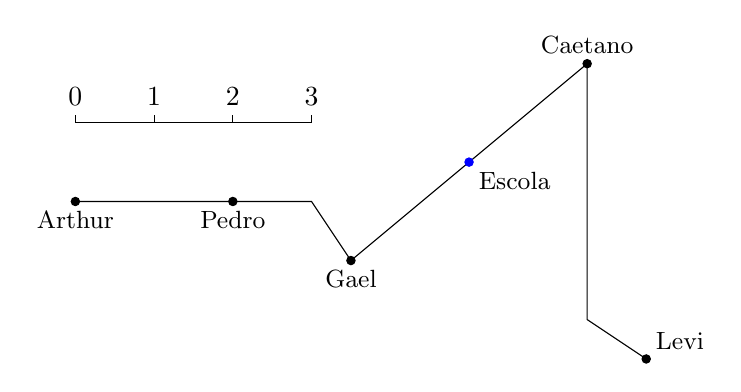
\begin{tikzpicture}
\tikzstyle{ponto}=[circle, minimum size=3pt, inner sep=0, draw=black, fill=black, shift only]
\draw(-2,2)grid(1,2.1);
\foreach \x in {0,1,2,3}
\node at (\x - 2,2.1)[above]{\x};
\coordinate (A) at (-2,1);
\coordinate (B) at (0,1);
\coordinate (C) at (1,1);
\coordinate (D) at (1.5,.25);
\coordinate (E) at (3,1.5);
\coordinate (F) at (4.5,2.75);
\coordinate (G) at (4.5,-.5);
\coordinate (H) at (5.25,-1);
\draw(A)--(B)--(C)--(D)--(E)--(F)--(G)--(H);
\node[ponto] at (A){};\node[ponto] at (B){};\node[ponto] at (D){};\node[ponto, blue] at (E){};\node[ponto] at (F){};\node[ponto] at (H){};
\node[below] at (A){\small Arthur};\node[below] at (B){\small Pedro };\node[below] at (D){\small Gael};\node[below right] at (E){\small Escola};\node[above] at (F){\small Caetano};\node[above right] at (H){\small Levi};
\end{tikzpicture}
\end{figure}

Os pontos marcados no plano cartesiano abaixo fornecem informações sobre a jornada de cada criança na última segunda-feira.
\phantomsection\label{\detokenize{AF106-5:fig-grafico-jornada}}

\begin{figure}[H]
\centering

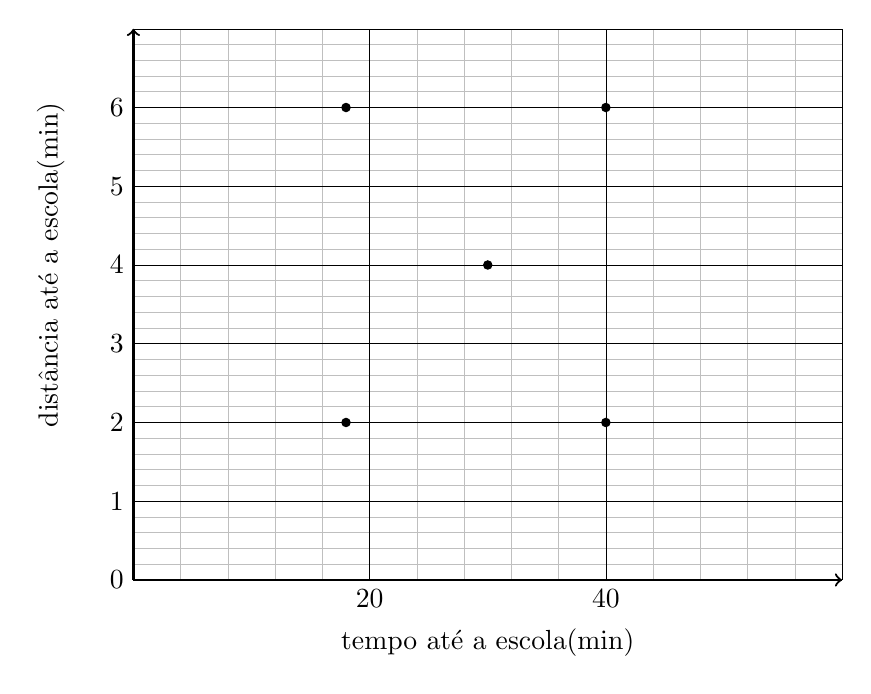
\begin{tikzpicture}
\tikzstyle{ponto}=[circle, minimum size=3pt, inner sep=0, draw=black, fill=black, shift only]
\begin{scope}[xscale=3]
\draw[help lines,xstep=.2,ystep=.2, lightgray] (0,0) grid (3,7);
\draw[help lines, black, xstep=1, ystep=1] (0,0) grid (3,7);
\draw[thick,->](0,0)--(3,0);
\draw[thick,->](0,0)--(0,7);
\draw(1.5,-.8)node{ tempo até a escola(min)};
\draw(-.35,4)node[rotate=90]{distância até a escola(min)};
\node[ponto] at(.9,2){};
\node[ponto] at(.9,6){};
\node[ponto] at(1.5,4){};
\node[ponto] at(2,2){};
\node[ponto] at(2,6){};
\foreach \y in {0,1, 2, 3, 4, 5, 6}
\draw(0,\y) [left] node {\y};
\draw(1,0)node[below]{20};
\draw(2,0)node[below]{40};
\end{scope}
\end{tikzpicture}
\end{figure}

\begin{enumerate}
\item {} 
Associe cada ponto do gráfico com o nome da criança que ele representa.

\item {} 
Como Pedro e Caetano foram para a escola na última segunda-feira? Por que?

\end{enumerate}

{\color{red}\bfseries{}{}`}\emph{{}`Adaptado de *The Language of Functions and Graphs}, Shell Centre for Mathematical Education Publications Ltd., 1985.

\end{task}

\begin{task}{ qual é o gráfico?}
\label{\detokenize{AF106-5:ativ-qual-e-o-grafico}}\label{\detokenize{AF106-5:atividade-qual-e-o-grafico}}

Dentre os gráficos apresentados a seguir identifique aquele que melhor descreve os dados apresentados em cada uma das tabelas seguintes.


\begin{enumerate}
\item  Café esfriando
\begin{table}[H]
\centering
\begin{tabu} to \textwidth{|c|c|c|c|c|c|c|c|}
\hline
\tcolor{Tempo (minutos)} & 0 & 5 & 10 & 15 & 20 & 25 & 30 \\
\hline
\tcolor{Temperatura ($^{\circ}$C)} & 90 & 79 & 70 & 62 & 55 & 49 & 44\\
\hline
\end{tabu}
\end{table}

\item Preparando a ceia

\begin{table}[H]
\centering
\begin{tabu} to \textwidth{|c|c|c|c|c|c|c|c|}
\hline
\tcolor{Peso (quilos)} & 3 & 4 & 5 & 6 & 7 & 8 & 9 \\
\hline
\tcolor{Tempo (horas)} & 2,5 & 3 & 3,5 & 4 & 4,5 & 5 & 5,5\\
\hline
\end{tabu}
\end{table}

\item Depois de três canecas de cerveja…

\begin{table}[H]
\centering
\begin{tabu} to \textwidth{|c|c|c|c|c|c|c|c|}
\hline
\tcolor{Tempo (horas)} & 1 & 2 & 3 & 4 & 5 & 6 & 7 \\
\hline
\tcolor{Álcool no sangue (mg/100ml)} & 90 & 75 & 60 & 45 & 30 & 15 & 0 \\
\hline
\end{tabu}
\end{table}

\item Como um bebê cresce antes do nascimento

\begin{table}[H]
\centering
\begin{tabu} to \textwidth{|c|c|c|c|c|c|c|c|c|}
\hline
\tcolor{Tempo de gestação (meses)} & 2 & 3 & 4 & 5 & 6 & 7 & 8 & 9 \\
\hline
\tcolor{Comprimento do bebê (cm)} & 4 & 9 & 16 & 24 & 30 & 34 & 38 & 42 \\
\hline
\end{tabu}
\end{table}
\end{enumerate}

\begin{figure}[H]
\centering

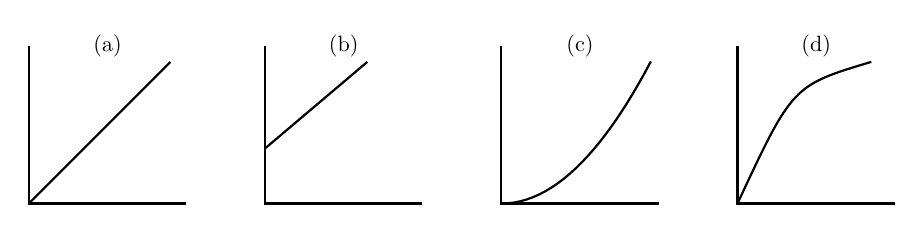
\begin{tikzpicture}
\draw[thick](0,2)--(0,0)--(2,0);
\draw(1,2)node[scale=.8]{(a)};
\draw[thick](0,0)--(1.8,1.8);
\begin{scope}[xshift=3cm]
\draw[thick](0,2)--(0,0)--(2,0);
\draw(1,2)node[scale=.8]{(b)};
\draw[thick](0,.7)--(1.3,1.8);
\begin{scope}[xshift=3cm]
\draw[thick](0,2)--(0,0)--(2,0);
\draw(1,2)node[scale=.8]{(c)};
\draw[domain=0:1.9,thick]plot(\x,.5*\x^2);
\begin{scope}[xshift=3cm]
\draw[thick](0,2)--(0,0)--(2,0);
\draw(1,2)node[scale=.8]{(d)};
\draw[thick](0,0).. controls (.7,1.5)..(1.7,1.8);
\end{scope}
\end{scope}
\end{scope}
\end{tikzpicture}

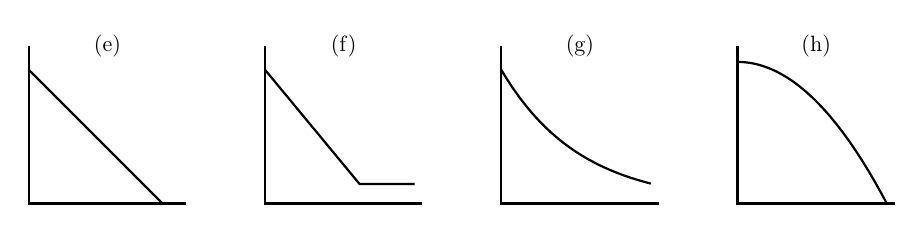
\begin{tikzpicture}
\draw[thick](0,2)--(0,0)--(2,0);
\draw(1,2)node[scale=.8]{(e)};
\draw[thick](0,1.7)--(1.7,0);
\begin{scope}[xshift=3cm]
\draw[thick](0,2)--(0,0)--(2,0);
\draw(1,2)node[scale=.8]{(f)};
\draw[thick](0,1.7)--(1.2,0.25)--(1.9,.25);
\begin{scope}[xshift=3cm]
\draw[thick](0,2)--(0,0)--(2,0);
\draw(1,2)node[scale=.8]{(g)};
\draw[domain=0:1.9,thick]plot(\x,{1.7*exp(-\x)});
\begin{scope}[xshift=3cm]
\draw[thick](0,2)--(0,0)--(2,0);
\draw(1,2)node[scale=.8]{(h)};
\draw[domain=0:1.9, thick]plot(\x,{(1.8-.5*\x^2} );
\end{scope}
\end{scope}
\end{scope}
\end{tikzpicture}

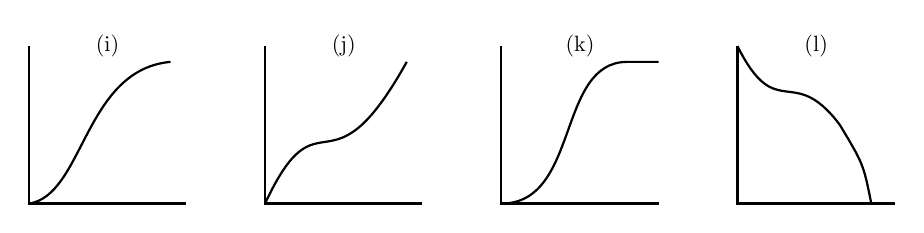
\begin{tikzpicture}
\draw[thick](0,2)--(0,0)--(2,0);
\draw(1,2)node[scale=.8]{(i)};
\draw[thick](0,0)..controls(.7,.1) and (.7,1.7) ..(1.8,1.8);
\begin{scope}[xshift=3cm]
\draw[thick](0,2)--(0,0)--(2,0);
\draw(1,2)node[scale=.8]{(j)};
\draw[thick](0,0)..controls(.7,1.5) and (.8,.0) ..(1.8,1.8);
\begin{scope}[xshift=3cm]
\draw[thick](0,2)--(0,0)--(2,0);
\draw(1,2)node[scale=.8]{(k)};
\draw[thick](0,0)..controls(1,0) and (.7,1.8) ..(1.6,1.8)..controls(1.9,1.8)..(2,1.8);
\begin{scope}[xshift=3cm]
\draw[thick](0,2)--(0,0)--(2,0);
\draw(1,2)node[scale=.8]{(l)};
\draw[thick](0,2)..controls(.5,1) and (.7,1.8) ..(1.3,1)..controls(1.6,.5)..(1.7,0);
\end{scope}
\end{scope}
\end{scope}
\end{tikzpicture}
\end{figure}

\(*\) Adaptado de \emph{The Language of Functions and Graphs}, Shell Centre for Mathematical Education Publications Ltd., 1985.
\end{task}

\begin{task}{ imaginando gráficos}
%\label{\detokenize{AF106-5:atividade-imaginando-graficos}}

Associe cada uma das situações apresentadas a seguir a um dos gráficos dados abaixo. Explique sua escolha e escreva, em cada um dos eixos, o que eles representam.
\begin{figure}[H]
\centering

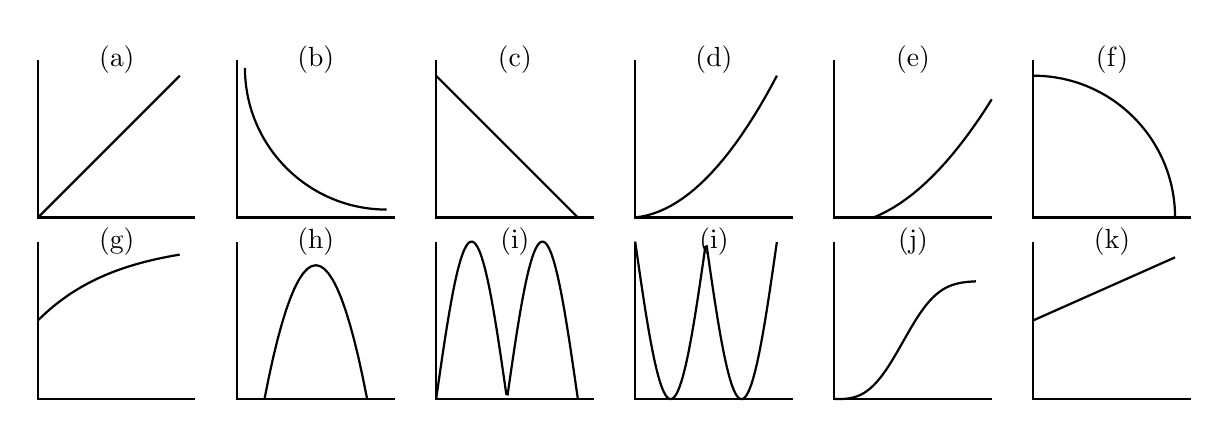
\begin{tikzpicture}
\node [matrix, column sep =.5cm] at (0,0)   {\draw[thick](0,2)--(0,0)--(2,0);\draw(1,2)node{(a)};\draw[thick](0,0)--(1.8,1.8);  &  \draw[thick](0,2)--(0,0)--(2,0);\draw(1,2)node{(b)};\draw[thick](0.1,1.9) arc(180:270:1.8);&\draw[thick](0,2)--(0,0)--(2,0);\draw(1,2)node{(c)};\draw[domain= 0:1.8,thick] plot(\x,1.8-\x); &\draw[thick](0,2)--(0,0)--(2,0);\draw(1,2)node{(d)};\draw[domain= 0:1.8,thick] plot(\x,.5*\x^2+.1*\x);&\draw[thick](0,2)--(0,0)--(2,0);\draw(1,2)node{(e)};\draw[domain= 0:2,thick] plot(\x,{max(0,.4*\x^2-.1)});&\draw[thick](0,2)--(0,0)--(2,0);\draw(1,2)node{(f)};\draw[thick](1.8,0) arc(0:90:1.8);\\  \draw[thick](0,2)--(0,0)--(2,0);\draw(1,2)node{(g)};\draw[domain=0:1.8,thick, samples=100]plot(\x, {2-exp(-\x)});& \draw[thick](0,2)--(0,0)--(2,0);\draw(1,2)node{(h)};\draw[domain=0.35:1.65,thick]plot(\x,{1.7-4*(1-\x)^2});& \draw[thick](0,2)--(0,0)--(2,0);\draw(1,2)node{(i)};\draw[domain=0:1.8, samples=100,thick]plot(\x,{abs(2*sin(200*\x))});&\draw[thick](0,2)--(0,0)--(2,0);\draw(1,2)node{(i)};\draw[domain=0:1.8, samples=100,thick]plot(\x,{2-(abs(2*sin(200*\x))});&\draw[thick](0,2)--(0,0)--(2,0);\draw(1,2)node{(j)};\draw[domain=0:1.8, samples=100,thick]plot(\x,{1.5-1.5*exp(-\x^3)});&       \draw[thick](0,2)--(0,0)--(2,0);\draw(1,2)node{(k)};\draw[thick](0,1)--(1.8,1.8);\\};
\end{tikzpicture}
\end{figure}

\begin{enumerate}[label=($\Roman*$)]
\item Após um concerto houve um grande silêncio. Então uma pessoa na platéia começou a aplaudir. Gradualmente, as pessoas à sua volta também começaram a apludir de forma que rapidamente todos estavam aplaudindo.

\item Se o preço cobrado pelo ingresso de um cinema for muito baixo, seu prorietário irá perder dinheiro. Por outro lado, se o valor cobrado for muito alto, poucas pessoas irão pagar e novamente o proprietário vai perder dinheiro. Um cinema deve portanto cobrar um preço moderado por seu ingresso de forma que seja lucrativo.

\item Preços estão agora subindo mais lentamente do que em qualquer época nos últimos cinco anos.
\end{enumerate}
\begin{itemize}
\item {} 
Adaptado do artigo \emph{Michal Ayalon \& Anne Watson \& Steve Lerman (2015). Progression Towards Functions: Students’ Performance on Three Tasks About Variables from Grades 7 to 12.}
\end{itemize}
\end{task}

\clearpage
\begin{reflection}
Observe as figuras abaixo
\begin{figure}[H]
\centering

\begin{tikzpicture}
\draw[->](0,0)--(2.5,0);
\draw[->](0,0)--(0,2.5);
\draw[domain=.2:2.2]plot (\x, \x+.2);
\foreach \x in{0.5,1,1.5}
\draw[dashed](\x,\x+.2)[->]--(\x+.5,\x+.2)--(\x+.5,\x+.7);
\foreach \x in{0.5,1,1.5}
\draw(\x+.2,\x+.15)--(\x+.2,\x+.25);
\foreach \x in{0.5,1,1.5}
\draw(\x+.25,\x+.15)--(\x+.25,\x+.25);
\begin{scope}[xshift=3cm]
\draw[->](0,0)--(2.5,0);
\draw[->](0,0)--(0,2.5);
\draw[domain=.2:2.3]plot(\x,{.3*(exp(\x))}) ;
\draw [->,dashed] (1.,0.4946163812100384) -- (1.,0.8154845485377135);
\draw [->,dashed] (1.5,0.8154845485377135) -- (1.5,1.3445067211014192);
\draw [->,dashed] (2.,1.3445067211014192) -- (2.,2.216716829679195);
\draw [dashed] (0.5,0.4946163812100384)-- (1.,0.4946163812100384);
\draw [dashed] (0.7274102214004744,0.5488318498488993) -- (0.7274102214004744,0.44040091257117747);
\draw [dashed] (0.7725897785995253,0.5488318498488993) -- (0.7725897785995253,0.44040091257117747);
\draw [dashed] (1.,0.8154845485377135)-- (1.5,0.8154845485377135);
\draw [dashed] (1.2274102214004736,0.8697000171765743) -- (1.2274102214004736,0.7612690798988525);
\draw [dashed] (1.2725897785995244,0.8697000171765743) -- (1.2725897785995244,0.7612690798988525);
\draw [dashed] (1.5,1.3445067211014192)-- (2.,1.3445067211014192);
\draw [dashed] (1.727410221400475,1.39872218974028) -- (1.727410221400475,1.290291252462558);
\draw [dashed] (1.7725897785995257,1.39872218974028) -- (1.7725897785995257,1.290291252462558);
\begin{scope}[xshift=3cm]
\draw[->](0,0)--(2.5,0);
\draw[->](0,0)--(0,2.5);
\draw[domain=.2:2.3]plot(\x,{2+(ln(\x))}) ;
\draw [->,dashed] (1.,1.3068528194400546) -- (1.,2.);
\draw [->,dashed] (1.5,2.) -- (1.5,2.4054651081081646);
\draw [->,dashed] (2.,2.4054651081081646) -- (2.,2.6931471805599454);
\draw [dashed] (0.5,1.3068528194400546)-- (1.,1.3068528194400546);
\draw [dashed] (0.7274102214004744,1.3610682880789153) -- (0.7274102214004744,1.2526373508011936);
\draw [dashed] (0.7725897785995253,1.3610682880789153) -- (0.7725897785995253,1.2526373508011936);
\draw [dashed] (1.,2.)-- (1.5,2.);
\draw [dashed] (1.2274102214004736,2.054215468638861) -- (1.2274102214004736,1.9457845313611395);
\draw [dashed] (1.2725897785995244,2.054215468638861) -- (1.2725897785995244,1.9457845313611395);
\draw [dashed] (1.5,2.4054651081081646)-- (2.,2.4054651081081646);
\draw [dashed] (1.727410221400475,2.4596805767470253) -- (1.727410221400475,2.3512496394693034);
\draw [dashed] (1.7725897785995257,2.4596805767470253) -- (1.7725897785995257,2.3512496394693034);
\end{scope}
\end{scope}
\begin{scope}[yshift=-3.5cm]
\draw[->](0,0)--(2.5,0);
\draw[->](0,0)--(0,2.5);
\draw[smooth,samples=100,domain=.2:2.2] plot(\x,{2.5-(\x)});
\draw [->,dashed] (1.,2.) -- (1.,1.5);
\draw [->,dashed] (1.5,1.5) -- (1.5,1.);
\draw [->,dashed] (2.,1.) -- (2.,0.5);
\draw [,dashed] (0.5,2.)-- (1.,2.);
\draw [dashed] (0.7274102214004744,2.054215468638861) -- (0.7274102214004744,1.9457845313611395);
\draw [dashed] (0.7725897785995253,2.054215468638861) -- (0.7725897785995253,1.9457845313611395);
\draw [dashed] (1.,1.5)-- (1.5,1.5);
\draw [dashed] (1.2274102214004736,1.5542154686388605) -- (1.2274102214004736,1.4457845313611388);
\draw [dashed] (1.2725897785995244,1.5542154686388605) -- (1.2725897785995244,1.4457845313611388);
\draw [dashed] (1.5,1.)-- (2.,1.);
\draw [dashed] (1.727410221400475,1.054215468638861) -- (1.727410221400475,0.9457845313611393);
\draw [dashed] (1.7725897785995257,1.054215468638861) -- (1.7725897785995257,0.9457845313611393);
\begin{scope}[xshift=3cm]
\draw[->](0,0)--(2.5,0);
\draw[->](0,0)--(0,2.5);
\draw[domain=.2:2.05]plot(\x,{2.5-.3*(exp(\x))}) ;
\draw [dashed] (0.7274102214004744,2.054215468638861) -- (0.7274102214004744,1.9457845313611395);
\draw [dashed] (0.7725897785995253,2.054215468638861) -- (0.7725897785995253,1.9457845313611395);
\draw [->,dashed] (1.,2.0053836187899616) -- (1.,1.6845154514622864);
\draw [->,dashed] (1.5,1.6845154514622864) -- (1.5,1.1554932788985808);
\draw [->,dashed] (2.,1.1554932788985808) -- (2.,0.2832831703208054);
\draw [dashed] (1.,1.6845154514622864)-- (1.5,1.6845154514622864);
\draw [dashed] (1.2274102214004736,1.7387309201011474) -- (1.2274102214004736,1.6302999828234255);
\draw [dashed] (1.2725897785995244,1.7387309201011474) -- (1.2725897785995244,1.6302999828234255);
\draw [dashed] (1.5,1.1554932788985808)-- (2.,1.1554932788985808);
\draw [dashed] (1.727410221400475,1.2097087475374417) -- (1.727410221400475,1.10127781025972);
\draw [dashed] (1.7725897785995257,1.2097087475374417) -- (1.7725897785995257,1.10127781025972);
\draw [dashed] (0.5,2.0053836187899616)-- (1.,2.0053836187899616);
\begin{scope}[xshift=3cm]
\draw[->](0,0)--(2.5,0);
\draw[->](0,0)--(0,2.5);
\draw[domain=.37:2.1]plot(\x,{1.0/(\x)}) ;
\draw [->,dashed] (1.,2.) -- (1.,1.);
\draw [->,dashed] (1.5,1.) -- (1.5,0.6666666666666666);
\draw [->,dashed] (2.,0.6666666666666666) -- (2.,0.5);
\draw [dashed] (0.7274102214004744,2.054215468638861) -- (0.7274102214004744,1.9457845313611395);
\draw [dashed] (0.7725897785995253,2.054215468638861) -- (0.7725897785995253,1.9457845313611395);
\draw [dashed] (1.,1.)-- (1.5,1.);
\draw [dashed] (1.2274102214004736,1.054215468638861) -- (1.2274102214004736,0.9457845313611393);
\draw [dashed] (1.2725897785995244,1.054215468638861) -- (1.2725897785995244,0.9457845313611393);
\draw [dashed] (1.5,0.6666666666666666)-- (2.,0.6666666666666666);
\draw [dashed] (1.727410221400475,0.7208821353055274) -- (1.727410221400475,0.6124511980278056);
\draw [dashed] (1.7725897785995257,0.7208821353055274) -- (1.7725897785995257,0.6124511980278056);
\draw [dashed] (0.5,2.)-- (1.,2.);
\end{scope}
\end{scope}
\end{scope}
\end{tikzpicture}
\end{figure}

O que os gráficos da primeira linha têm em comum? E as da segunda linha?

Agora observe-os por coluna. Você consegue identificar algo em comum?
\end{reflection}

\begin{description}
\item[{Função crescente e função decrescente\index{Função crescente e função decrescente|textbf}}] \leavevmode\phantomsection\label{\detokenize{AF106-5:term-funcao-crescente-e-funcao-decrescente}}
Uma função \(f: \mathbb{R} \to \mathbb{R}\) é dita \emph{crescente} quando os valores das imagens, \(f(x)\), aumentam à medida em que os valores de \(x\) aumentam, ou seja, para \(x_2>x_1\) tem-se \(f(x_2)>f(x_1)\).

\begin{figure}[H]
\centering

\begin{tikzpicture}
\draw[thick,->](-2,0)--(5,0);
\draw[thick,->](0,-1)--(0,4);
\draw[very thick,domain=-2:2.9, \currentcolor!80]plot(\x,{.5+.2*exp(\x)});
\draw[thick,dashed, ->](1,{.5+.2*exp(1)})--(2.5,{.5+.2*exp(1)})--(2.5,{.5+.2*exp(2.5)}) ;
\end{tikzpicture}
\end{figure}

E é dita \emph{decrescente} quando os valores das imagens, \(f(x)\), diminuem à medida em que os valores de \(x\) aumentam, ou seja, para \(x_2>x_1\) tem-se \(f(x_2)<f(x_1)\).
\begin{figure}[H]
\centering

\begin{tikzpicture}
\draw[thick,->](-2,0)--(5,0);
\draw[thick,->](0,-1)--(0,4);
\draw[very thick,domain=-2:3.6, \currentcolor!80]plot(\x,{3-.1*exp(\x)});
\draw[thick,dashed, ->](1,{3-.1*exp(1)})--(3,{3-.1*exp(1)})--(3,{3-.1*exp(3)}) ;
\end{tikzpicture}
\end{figure}

\end{description}


\begin{task}{ leia no gráfico!}
\label{\detokenize{AF106-5:atividade-leia-no-grafico}}\label{\detokenize{AF106-5:ativ-praticando-notacao}}

Seja \(f\) a função real cuja representação gráfica é apresentada a seguir.

\begin{figure}[H]
\centering

\begin{tikzpicture}
\tikzstyle{ponto}=[circle, minimum size=3pt, inner sep=0, draw=black, fill=black, shift only]
\draw[gray!40](0,-1.5)grid[xstep=.25,ystep=.25,line width =1pt](5.5,3);
\draw(0,-1.5)grid[xstep=1,ystep=1,line width =1pt, help lines](5.5,3);
\draw[->,thick](-.5,0)--(5.5,0) node[right]{$x$};
\draw[->,thick](0,-1.5)--(0,3)node[above]{$y$};
\draw[very thick, \currentcolor!80](0,-.5)--(.5,1)--(1,1.5)--(1.5,1.5)--(2,.5)--(2.5,0)--(3,-1)--(4,2)--(4.5,2.5)--(5,2.75);
\foreach \x in{2, 4, 6, ..., 10}
\draw(.5*\x,0)[below]node{\x};
\foreach \y in{-2, 2,4,6}
\draw(0,.5*\y)[left]node{\y};
\node[below left]at (0,0){0};
\end{tikzpicture}
\end{figure}

A partir da representação gráfica calcule os seguintes valores:

\begin{table}[H]
\centering
\begin{tabu} to \textwidth{|l|c|}
\hline
\thead
Notação & Valor \\
\hline
\(f(1)-f(0)\) & \\
\hline
\(4\cdot f(3)\) & \\
\hline
\(f(4)/f(2)\) & \\
\hline
\(f(6)\cdot f(2)\) & \\
\hline
\(x\) quando \(f(x)=-2\) & \\
\hline
\(x\) quando \(f(x)=0\) & \\
\hline
\(f(3\cdot 2)-4\cdot f(\sqrt{81})+1\) & \\
\hline
\end{tabu}
\end{table}

\end{task}

\begin{reflection}
Observe o gráfico da função real dada pela expressão \(f(x)=3x^2-15x+18\). Veja que ele possui interseções com o eixo das abscissas e com o eixo das ordenadas. Qual procedimento você utilizaria para determinar esses pontos de interseção?
\begin{center}\begin{tikzpicture}
\draw[->, thick](-.5,0)--(4,0);
\draw[->,thick](0,-.5)--(0,6);
\draw[very thick, domain=-.2:3.7, samples=100, \currentcolor!80]plot(\x,{1.5*(\x-1.5)*(\x-2)});
\end{tikzpicture}\end{center}
Os valores de \(x\) para os quais há interseção com o eixo das abscissas são chamados de \emph{zeros} da função.
\end{reflection}

\begin{task}{Imposto de renda}

A seguinte tabela é utilizada para o cálculo do Imposto de Renda para Pessoa Física (IRPF).

\begin{table}[H]
\centering

\large{\textbf{Tabela do IRF - Vigência a partir de 01/04/2015}}

(Medida Provisória 670/2015 convertida na Lei 13.149/2015)
\begin{tabu} to \textwidth{|l|c|r|}
\hline
\thead
Base de cálculo (R\$) & Alíquota (\%) & Parcela a deduzir do IR (R\$) \\
\hline
Até $1.903{,}98$ & - & - \\
\hline
De $1.903{,}99$ até $2.826{,}65$ & 7,5 & $142{,}80$ \\
\hline
De 2$.825{,}55$ até $3.751{,}05$ & 15 & $354{,}80$ \\
\hline
$3.751{,}06$ até $4.664{,}68$ & 22,5 & $636{,}13$ \\
\hline
Acima de $4.664{,}68$ & 27,5 & $869{,}36$ \\
\hline
\end{tabu}
\caption{Fonte: \url{http://www.portaltributario.com.br}}
\end{table}

Por esta tabela, um trabalhador cujo rendimento é inferior a R\$ $1.903{,}98$ está isento do imposto de renda. Já um trabalhador com rendimento de R\$ $3.000{,}00$ tem um desconto, em reais, de $15\%$ de $3.000{,}00$ (450,00) menos a dedução de 354,80, isto é, deverá pagar de importo de renda o valor $450-354{,}80=95{,}20$R\$.

\clearpage
\begin{enumerate}
\item Com os dados apresentados na tabela acima construímos a seguinte função que fornece o valor de importo de renda a ser pago, a partir do rendimento informado:
\[f(x)=
\begin{cases}
0, \text{ se } x\leq1.903{,}98\\
0{,}075x-142{,}90, \text{ se } 1.903{,}98<x<2.826{,}65\\
0{,}15x-354{,}90, \text{ se } 2.826{,}65\leq x<3.751{,}05\\
0{,}225x-636{,}13 \text{ se } 3.751{,}05 \leq x<4.664{,}68\\
0{,}275x-869{,}36 \text{ se } 4.664{,}68\leq x
\end{cases}
\]

Determine o imposto que deverá ser pago por um trabalhador cujo rendimento seja:
\begin{enumerate}
\item R\$ $1.750{,}00$
\item R\$ $2.680{,}00$
\item R\$ $4.060{,}00$
\item R\$ $5.500{,}00$
\end{enumerate}

\item Observe o gráfico a seguir. Nele estão destacados os impostos de renda pago por três trabalhadores, indicados pelas letras $A$, $B$ e $C$.

\begin{figure}[H]
\centering

\begin{tikzpicture}[xscale=.2,yscale=1.25]
\draw [->] (0,0) -- (52,0) node [below left, scale=.75] {Salários (R\$)};
\draw [->] (0,0) -- (0,5) node [above left, rotate=90, scale=.75] {Imposto (R\$)};

\draw [thick, \currentcolor!80] (0,0) -- (19.0390,0) -- (28.2665,28.25665*.075-1.428) -- (37.506,37.056*.15-3.548) -- (46.64468,46.64468*.225-6.3613) -- (50,50*.275-8.6936);

\draw [dashed,\currentcolor!80](28.2665,28.25665*.075-1.428) -- (28.2665,0);
\draw [dashed,\currentcolor!80] (37.506,37.056*.15-3.548) -- (37.506,0);
\draw [dashed,\currentcolor!80](46.64468,46.6468*.225-6.3613) -- (46.64468,0);

\draw [dashed] (0,.552) -- (26,.552) -- (26,0);
\draw [dashed] (0,1.522) -- (34,1.552) -- (34,0);
\draw [dashed] (0,2.6387) -- (40.3,2.6387) -- (40.3,0); 

\node (a) [circle,fill, inner sep=1pt,label=above:A] at (26,.522) {};
\node (b) [circle,fill, inner sep=1pt, label=above:B] at (34,1.522) {};
\node (c) [circle,fill, inner sep=1pt, label=above:C, xshift=.5mm] at (40,2.6387) {};

\node [left] at (0,.522) {52,20};
\node [left] at (0,1.5520) {155,20};
\node [left] at (0,2.6387) {263,87};
\end{tikzpicture}
\end{figure}

Segundo a tabela IRF, determine as alíquotas de desconto que estão sendo aplicadas a cada um destes trabalhadores e qual o salário de cada um deles.
\end{enumerate}

\end{task}

\clearpage
\begin{task}{Planos telefônicos}

Você deseja trocar o plano do seu telefone e ao consultar a sua operadora tem a opção de escolher entre dois planos: plano Prata e plano Ouro. No seu plano atual, você paga R\$ $70{,}00$ por 500MB de internet e os dados além disso custam R\$ $0{,}20$ por MB. 

O plano Ouro cobra R\$ $140{,}00$ por dados ilimitados e o plano Prata tem a mesma estrutura do seu plano atual. Os valores cobrados pelo plano Prata estão representados no gráfico a seguir.

\begin{figure}[H]
\centering


\begin{tikzpicture}[yscale=.5,scale=.75, every node/.style={scale=.75}]

\draw [->] (0,0) -- (14,0) node [below left, yshift=-.5cm] {Dados (MB)};
\draw [->] (0,0) -- (0,20) node [above left, rotate=90, yshift=.5cm] {Valor (R\$)};
\draw [help lines] (0,0) grid (14,20);

\foreach \x in {2,4,...,20} \node [left] at (0,\x) {\x0};
\foreach \x in {1,2,...,14} \node [below] at (\x,0) {\x00};

\node [below left] at (0,0) {0};

\draw [thick, \currentcolor!80] (0,8) -- (6,8) -- (14,20);

\end{tikzpicture}
\end{figure}

\begin{enumerate}
\item Qual o valor fixo cobrado no plano Prata e que quantidade de dados ele cobre?
\item Qual o valor por MB excedente do valor estipulado?
\item A partir de que quantidade de dados consumidos o plano Ouro passa a ser mais vantajoso?
\item Represente no sistema de coordenadas acima o gráfico do preço a pagar pelo plano Ouro.
\end{enumerate}

\end{task}

\clearpage

\begin{task}{Bandeiras tarifárias}

Desde o ano de 2015, as contas de energia passaram a trazer uma novidade: o Sistema de Bandeiras Tarifárias, que apresenta as seguintes modalidades: verde, amarela e vermelha - as mesmas cores dos semáforos - e indicam se haverá ou não acréscimo no valor de energia a ser repassada ao consumidor final, em função das condições de geração de eletricidade. Cada modalidade apresenta as seguintes características:


\begin{itemize}
\item[
{\begin{tikzpicture}[scale=.5,remember picture, overlay, shift={(-1,-.75))}]
      \draw [very thick] (0,-.25) -- (0,1);
      \draw [fill=session2] (0,1) .. controls (.25,1.25) and (.75,.75) .. (1,1) -- (1,.5) .. controls (.75,.25) and (.25,.75) .. (0,.5) -- cycle;
      \end{tikzpicture}}]

 \textbf{Bandeira verde}: condições favoráveis de geração de energia. A tarifa não sofre nenhum acréscimo;

\item[{\begin{tikzpicture}[scale=.5,remember picture, overlay, shift={(-1,-.75))}]
      \draw [very thick] (0,-.25) -- (0,1);
      \draw [fill=box2!50!yellow] (0,1) .. controls (.25,1.25) and (.75,.75) .. (1,1) -- (1,.5) .. controls (.75,.25) and (.25,.75) .. (0,.5) -- cycle;
      \end{tikzpicture}}]

\textbf{Bandeira amarela}: condições de geração menos favoráveis. A tarifa sobre acréscimo de R\$ $0{,}01343$ para cada quilowatt-hora (kWh) consumidos;

\item[{\begin{tikzpicture}[scale=.5,remember picture, overlay, shift={(-1,-.75))}]
      \draw [very thick] (0,-.25) -- (0,1);
      \draw [fill=session3!50!red!90!white] (0,1) .. controls (.25,1.25) and (.75,.75) .. (1,1) -- (1,.5) .. controls (.75,.25) and (.25,.75) .. (0,.5) -- cycle;
      \end{tikzpicture}}]

\textbf{Bandeira vermelha - patamar 1}: condições mais custosas de geração. A tarifa sofre acréscimo de R\$ $0{,}04169$ para cada quilowatt-hora (kWh) consumido.

\item[{\begin{tikzpicture}[scale=.5,remember picture, overlay, shift={(-1,-.75))}]
      \draw [very thick] (0,-.25) -- (0,1);
      \draw [fill=session3] (0,1) .. controls (.25,1.25) and (.75,.75) .. (1,1) -- (1,.5) .. controls (.75,.25) and (.25,.75) .. (0,.5) -- cycle;
      \end{tikzpicture}}]

\textbf{Bandeira vermelha - patamar 2}: condições mais custosas de geração. A tarifa sofre acréscimo de R\$ $0{,}06243$ para cada quilowatt-hora (kWh) consumido.
\end{itemize}

\flushright{\small

Texto extraído da página da ANEEL em 28/03/2020 \\ \url{https://www.aneel.gov.br/bandeiras-tarifárias}}

\justify
O sistema de coordenadas abaixo contém os gráficos para as funções que relacionam o preço a pagar pela energia em relação ao consumo em quilowatt-hora (kWh) para cada uma das bandeiras tarifárias, em uma cidade vizinha. Com base nas informações do gráfico a seguir, responda:

\begin{figure}[H]
\centering

\begin{tikzpicture}[yscale=2.5,scale=.75, every node/.style={scale=.75}]

\draw [->] (0,5) -- (11,5) node [below left, yshift=-.5cm] {consumo (kWh)};
\draw [->] (0,5) -- (0,9) node [above left, , rotate=90, yshift=1.5cm, overlay] {Preço a pagar (R\$)};

\foreach \x in {2,4,...,10} {\node [below] at (\x,5) {\x00};
\draw [help lines] (\x,5) -- (\x,9);
};
\foreach \x/\y in {8/{800,00},8.1343/{813,43},8.4169/{841,89},8.6243/{862,43}} {

\node [left,overlay] at (0,\x) {\y};

\draw [thick, \currentcolor!80] (0,5) -- (10,\x);
\draw [help lines] (0,\x) -- (10,\x);
};

\end{tikzpicture}
\end{figure}

\end{task}

\clearpage
\def\currentcolor{session3}
\begin{objectives}{Todo mundo tem Facebook?}
{
\begin{itemize}

\item Utilizar os conhecimentos adquiridos ao longo do Capítulo para investigar o crescimento do número de usuários ativos na rede social Facebook.

\item Fazer inferência baseado em um modelo matemático.

\end{itemize}
}{1}{1}
\end{objectives}
\begin{sugestions}{Todo mundo tem Facebook?}
{
\begin{itemize}
\item No item (e) os dados indicam que o número de usuários não irá ultrapassar $1.500.000.000$, mas isso pode não ser facilmente percebido. Espera-se, caso o estudante acredite que o número de usuários atinja os $2$ bilhões, que isso ocorra depois de um grande intervalo de tempo.
\end{itemize}
}{1}{1}
\end{sugestions}
\clearmargin
\begin{answer}{Todo mundo tem Facebook?}
{
\begin{enumerate}
\item $19999900\% , 450\%, 118\%, 483\%, 114\%, 147\%, 62\%, 33\%, 32\%, 16\%, 7\%$.

\item\adjustbox{valign=t}{
\resizebox{.9\linewidth}{!}
{
\begin{tikzpicture}[scale=1.5, every node/.style={black}, every path/.style={black}]
\draw [help lines, xstep=.5cm,ystep=.25cm] (-.1,-.1) grid (7.5,4.1);
\foreach \x in {0,1, 2,3, 4, 5, 6,7,8,9,10,11,12,13,14, 15}
\draw[shift={(.5*\x,0)},color=black] (0pt,-2pt) -- (0pt,-2pt) node[below] { $\x$};
\foreach \y in {100,200,300,400,500,600,700,800,900,1000,1100,1200,1300,1400,1500,1600}
\draw[shift={(-.3,.18 +.0025*\y)},color=black] (0pt,-2pt) -- (0pt,-2pt) node[below] { $\y$};
\draw[thick, ->](-.1,0)--(7.6,0);
\draw[thick, ->](0,-.1)--(0,4.1);
\draw[fill =session1](.5,0) circle(1pt);
\draw[fill =session1](1,.06) circle(1pt);
\draw[fill =session1](1.5,.08) circle(1pt);
\draw[fill =session1](2,.09) circle(1pt);
\draw[fill =session1](2.5,.2) circle(1pt);
\draw[fill =session1](3,.37) circle(1pt);
\draw[fill =session1](3.5,.92) circle(1pt);   
\draw[fill =session1](4,1.5) circle(1pt);
\draw[fill =session1](4.5,2) circle(1pt);
\draw[fill =session1](5,2.62) circle(1pt);
\draw[fill =session1](5.5,3.08) circle(1pt);
\draw[fill =session1](6,3.35) circle(1pt);
\end{tikzpicture}
}}
\end{enumerate}
}{1}
\end{answer}
\mspace{.25em}
\begin{answer}{Todo mundo tem Facebook?}
{
\begin{enumerate}\setcounter{enumi}{2}
\item No primeiro ano, observa-se um grande crescimento no número de usuários ativos, entre os anos de $2006$ e $2010$, o crescimento percentual oscila e, a partir de $2011$, é cada vez menor, indicando que o crescimento do número de usuários está com tendência a diminuir.

\item Espera-se para $2016$ um valor acima de $1.317.000.000$ e abaixo de $1.400.000.000$. Para $2017$ um valor maior que o anterior e que não ultrapasse $1.500.000.000$.

\item É razoável imaginar que o número de usuários continuará a aumentar. Com um crescimento percentual cada vez menor a tendência observada é que a marca de $2$ bilhões de usuários não será atingida.

\item Para o ano de $2013$ tem-se $f(9)=1.055.876.085$ e para o ano de $2014$ tem-se $f(10)=1.220.936.348$.

\item Para o ano de $2016$ o modelo prevê um número de usuários de $f(12)=1.359.620.842$ e para $2017$, $f(13)=1.381.536.488$.

\end{enumerate}
}{1}
\end{answer}
\begin{objectives}{Decodificando a mensagem}
{
\begin{itemize}

\item Estabelecer modelo matemático a partir de funções, mais especificamente, em uma situação que envolve codificação de mensagens.

\item Compreender intuitivamente as condições necessárias para a existência da inversa de uma função. (injetividade e sobrejetividade)

\end{itemize}
}{1}{2}
\end{objectives}
\begin{sugestions}{Decodificando a mensagem}
{
\begin{itemize}
\item Na solução do item \titem{d)} estimule seus estudantes a descrever com palavras de maneira precisa o que acontece com os números maiores que $26$ caso ele use a expressão $f(x)=x+14$.
\end{itemize}
}{1}{1}
\end{sugestions}
\begin{answer}{Decodificando a mensagem}
{
\begin{enumerate}
\item XBPVTB

\item Usaria a linha debaixo para descobrir a letra original correspondente: CRIPTOGRAFAR.

\item Resposta pessoal
\end{enumerate}
}{1}
\end{answer}

\begin{answer}{Decodificando a mensagem}
{
\begin{enumerate}\setcounter{enumi}{3}
\item Uma resposta possível seria:

\end{enumerate}
\begin{table}[H]
\centering
\resizebox{\linewidth}{!}
{
\setlength\tabcolsep{2.5pt}
\begin{tabu} to \textwidth{|c|*{26}{>{$}c<{$}|}}
\hline
\cellcolor{\currentcolor!80}{\textcolor{white}{\textbf{Original}}} & 1 & 2 & 3 & 4 & 5 & 6 & 7 & 8 & 9 & 10 & 11 & 12 & 13 & 14 & 15 & 16 & 17 & 18 & 19 & 20 & 21 & 22 & 23 & 24 & 25 & 26 \\
\hline
\cellcolor{\currentcolor!80}{\textcolor{white}{\textbf{Código}}} & 16 & 17 & 18 & 19 & 20 & 21 & 22 & 23 & 24 & 25 & 26 & 1 & 2 & 3 & 4 & 5 & 6 & 7 & 8 & 9 & 10 & 11 & 12 & 13 & 14 & 15 \\
\hline
\end{tabu}}
\end{table}

Outra possibilidade é escrever $f(x)=x+15$, subtraindo $26$ se $f(x)$ for maior que $26$.

\begin{enumerate}\setcounter{enumi}{4}

\item\adjustbox{valign=t}
{
\resizebox{.9\linewidth}{!}
{
\begin{tikzpicture}[every node/.style={black}, every path/.style={black}]
\draw[scale=.5](0,0)grid(26,26);
\foreach \i [count=\x from 0] in{{A}, {B},{C}, {D}, {E}, {F}, {G}, {H},{I},{J},{K},{L},{M},{N},{O},{P},{Q},{R},{S},{T},{U},{V},{W},{X},{Y},{Z}}
\draw (.2+.5*\x,-.4) node {\i};
\foreach \i [count=\x from 0] in{{A}, {B},{C}, {D}, {E}, {F}, {G}, {H},{I},{J},{K},{L},{M},{N},{O},{P},{Q},{R},{S},{T},{U},{V},{W},{X},{Y},{Z}}
\draw (-.4,.2+.5*\x) node {\i};
\fill[color=\currentcolor!80] ( 0.0 , 0.0 )--( 0.5 , 0.0 )--( 0.5 , 0.5 )--( 0.0 , 0.5 );
\fill[color=\currentcolor!80] ( 0.5 , 1.5 )--( 1.0 , 1.5 )--( 1.0 , 2.0 )--( 0.5 , 2.0 );
\fill[color=\currentcolor!80] ( 1.0 , 4.0 )--( 1.5 , 4.0 )--( 1.5 , 4.5 )--( 1.0 , 4.5 );
\fill[color=\currentcolor!80] ( 1.5 , 7.5 )--( 2.0 , 7.5 )--( 2.0 , 8.0 )--( 1.5 , 8.0 );
\fill[color=\currentcolor!80] ( 2.0 , 12.0 )--( 2.5 , 12.0 )--( 2.5 , 12.5 )--( 2.0 , 12.5 );
\fill[color=\currentcolor!80] ( 2.5 , 4.5 )--( 3.0 , 4.5 )--( 3.0 , 5.0 )--( 2.5 , 5.0 );
\fill[color=\currentcolor!80] ( 3.0 , 11.0 )--( 3.5 , 11.0 )--( 3.5 , 11.5 )--( 3.0 , 11.5 );
\fill[color=\currentcolor!80] ( 3.5 , 5.5 )--( 4.0 , 5.5 )--( 4.0 , 6.0 )--( 3.5 , 6.0 );
\fill[color=\currentcolor!80] ( 4.0 , 1.0 )--( 4.5 , 1.0 )--( 4.5 , 1.5 )--( 4.0 , 1.5 );
\fill[color=\currentcolor!80] ( 4.5 , 10.5 ) rectangle ( 5.0 , 11.0 );
\fill[color=\currentcolor!80] ( 5.0 , 8.0 ) rectangle ( 5.5 , 8.5 );
\fill[color=\currentcolor!80] ( 5.5 , 6.5 ) rectangle ( 6.0 , 7.0 );
\fill[color=\currentcolor!80] ( 6.0 , 6.0 ) rectangle ( 6.5 , 6.5 );
\fill[color=\currentcolor!80] ( 6.5 , 6.5 ) rectangle ( 7.0 , 7.0 );
\fill[color=\currentcolor!80] ( 7.0 , 8.0 ) rectangle ( 7.5 , 8.5 );
\fill[color=\currentcolor!80] ( 7.5 , 10.5 ) rectangle ( 8.0 , 11.0 );
\fill[color=\currentcolor!80] ( 8.0 , 1.0 ) rectangle ( 8.5 , 1.5 );
\fill[color=\currentcolor!80] ( 8.5 , 5.5 ) rectangle ( 9.0 , 6.0 );
\fill[color=\currentcolor!80] ( 9.0 , 11.0 ) rectangle ( 9.5 , 11.5 );
\fill[color=\currentcolor!80] ( 9.5 , 4.5 ) rectangle ( 10.0 , 5.0 );
\fill[color=\currentcolor!80] ( 10.0 , 12.0 ) rectangle ( 10.5 , 12.5 );
\fill[color=\currentcolor!80] ( 10.5 , 7.5 ) rectangle ( 11.0 , 8.0 );
\fill[color=\currentcolor!80] ( 11.0 , 4.0 ) rectangle ( 11.5 , 4.5 );
\fill[color=\currentcolor!80] ( 11.5 , 1.5 ) rectangle ( 12.0 , 2.0 );
\fill[color=\currentcolor!80] ( 12.0 , 0.0 ) rectangle ( 12.5 , 0.5 );
\fill[color=\currentcolor!80] ( 12.5 , 12.5 ) rectangle ( 13.0 , 13.0 );
\draw(12.3,-1)node{alfabeto};
\draw(-1,12.3) node[rotate=90.]{Código};   
\end{tikzpicture}
}
}

Para valores maiores que $26$ devemos subtrair $26$ sucessivamente até encontrar um valor positivo menor que ou igual a $26$ e então encontrar a letra correspondente. Isso equivale a tomar o resto da divisão por $26$.


\item Impossível decodificar, pois os códigos P, Q e X não têm correspondente no alfabeto e os códigos G e J têm mais de uma opção de escolha.

\item Códigos de D a K têm duas letras do alfabeto associadas a cada um. Códigos de P a T e de X a Z não têm correspondente no alfabeto.

\item Todo código deve possuir um único correspondente no alfabeto. Ou seja, a relação (código, alfabeto) deve ser uma função.

\end{enumerate}
}{1}
\end{answer}

\know{}
\label{\detokenize{AF106-A::doc}}\label{\detokenize{AF106-A:para-saber-mais}}\label{\detokenize{AF106-A:sec-aprofundando-grafico}}

\begin{task}{ Todo mundo tem \emph{Facebook}?}
\label{\detokenize{AF106-A:atividade-todo-mundo-tem-facebook}}\label{\detokenize{AF106-A:ativ-todo-mundo-tem-facebook}}

A rede social virtual \emph{Facebook} é um grande sucesso. O Facebook criado por Mark Zuckerberg em outubro de 2003, com o nome de \emph{Facemash}, quando ele era  um estudante do segundo ano em Harvard. Inicialmente \(450\) visitantes geraram \(22.000\) visualizações de fotos em suas primeiras \(4\) horas online. Em fevereiro de \(2004\), agora com o nome de \emph{Thefacebook}, ele já contava com a participação de mais da metade dos alunos de Harvard, e um mês depois, estudantes das Universidades de Stanford, Columbia, Yale, Boston, Nova Iorque e MIT tiveram acesso à rede social criada por Mark Zuckerberg. A partir de setembro de \(2005\), funcionários de várias empresas, dentre elas \emph{Apple} e \emph{Microsoft}, puderam ter acesso ao \emph{Facebook} e no final de \(2006\) o serviço ficou disponível para qualquer pessoa maior de \(13\) anos e com um endereço válido de \emph{e-mail}.

A tabela a seguir mostra o número de usuários ativos do \emph{Facebook} em janeiro dos anos de \(2004\) a \(2015\).

\begin{table}[H]
\centering
\begin{tabu} to \textwidth{|c|l|c|}
\hline
\thead
Ano & Número de usuários & Crescimento percentual \\
\hline
2004 & 5 & \textendash{} \\
\hline
2005 & 1.000.000 & \\
\hline
2006 & 5.500.000 & 450\% \\
\hline
2007 & 12.000.000 & \\
\hline
2008 & 70.000.000 & \\
\hline
2009 & 150.000.000 & \\
\hline
2010 & 370.000.000 & \\
\hline
2011 & 600.000.000 & \\
\hline
2012 & 800.000.000 & \\
\hline
2013 & 1.056.000.000 & \\
\hline
2014 & 1.228.000.000 & \\
\hline
2015 & 1.317.000.000 & \\
\hline
\end{tabu}
\end{table}


Imagine que queremos investigar o crescimento anual do número de usuários. E, a partir da investigação formular um modelo que nos permita fazer previsões sobre a base de usuários para os próximos anos.
\begin{enumerate}
\item {} 
Vamos começar investigando o crescimento percentual, preenchendo as lacunas da terceira coluna da tabela acima.

\item {} 
Marque no plano cartesiano os pontos correspondentes aos dados fornecidos pelas duas primeiras colunas da tabela, usando a seguinte escala: no eixo das abscissas \(1\) cm corresponde a \(1\) ano e no eixo das ordenadas \(1\) cm corresponde a \(200\) milhões de usuários ativos.

\item {} 
Como você descreveria o crescimento do número de usuários ativos do \emph{Facebook}? Você acha que o crescimento está com tendência a diminuir, a aumentar ou a permanecer estável?

\item {} 
Baseado no item c), faça uma previsão para o número de usuários para os anos de 2016 e 2017.

\item {} 
Usando os dados da tabela e a representação gráfica feita no item b), faça uma previsão para o futuro do \emph{Facebook}. Você acha que os números continuarão a aumentar? Se sim, quando ele atingirá a marca de \(2\) bilhões de usuários? Explique seu raciocínio.

\item {} 
Um modelo matemático que fornece uma aproximação para a relação entre os dados das duas primeiras colunas da tabela é dado por uma função \(f\) que tem a seguinte expressão
\begin{equation*}
\begin{split}f(x)=\dfrac{980}{0,7+670 \cdot 0,45^{(x+1)}}\end{split}
\end{equation*}
em que \(x\) representa o tempo decorrido desde \(2004\), isto é, para \(2010\) tem-se \(x=6\), e \(f(6)\) é o valor em milhões de usuários ativos no \emph{Facebook} naquele ano. Com a ajuda de uma calculadora científica, use a expressão acima para calcular a estimativa do número de usuários nos anos de \(2013\) e de \(2014\), e em seguida compare com a tabela.

\item {} 
Use a expressão anterior e calcule a estimativa para os anos de \(2016\) e \(2017\) e compare com as suas previsões do item (d).

\end{enumerate}

Os dados reais para os meses de janeiro de \(2016\) e \(2017\) são \(1.654.000.000\) e \(1.936.000.000\), respectivamente. Isso significa que apesar do modelo descrever de forma satisfatória o comportamento do crescimento do número de usuários até o ano de \(2015\), para os anos seguintes ele não se mostra adequado. Existia de fato uma tendência para diminuição do crescimento, no entanto essa trajetória foi possivelmente modificada por ações que foram tomadas pela empresa ao perceber tal comportamento.

Situações como essa são bastante comuns em Modelagem Matemática. O modelo se mostra adequado sob certas condições, mas quando outras variáveis são consideradas (investimento em propaganda, alteração no algoritmo que escolhe as atualizações que serão exibidas para cada usuário, etc) ele pode perder sua acurácia, momento em que se fazem necessárias revisões.

\end{task}

\begin{task}{ Decodificando a mensagem}
\label{\detokenize{AF106-A:atividade-decodificando-a-mensagem}}\label{\detokenize{AF106-A:ativ-decodificando}}

Um dos conceitos mais importantes para a segurança na \emph{internet} nos dias de de hoje é o que chamamos de \textbf{criptografia} (do grego \emph{criptos} = escondido, \emph{grafia} = escrita). Segundo o site \emph{wikipedia} ela é o estudo dos princípios e técnicas pelas quais a informação pode ser transformada da sua forma original para outra codificada, de forma que possa ser conhecida apenas por seu destinatário (detentor da “chave secreta”), o que a torna difícil de ser decifrada por alguém não autorizado. Em outras palavras, cria-se um código que pode ser facilmente desfeito (decodificado) mas apenas por aqueles que conhecem a codificação.

Considere a seguinte maneira de codificar o alfabeto

\begin{table}[H]
\centering
\setlength\tabcolsep{3pt}
\begin{tabu} to \textwidth{|c|c|c|c|c|c|c|c|c|c|c|c|c|c|c|c|c|c|c|c|c|c|c|c|c|c|c|}
\hline
\cellcolor{\currentcolor!80}{\textcolor{white}{\textbf{Original}}} & A & B & C & D & E & F & G & H & I & J & K & L & M & N & O & P & Q & R & S & T & U & V & W & X & Y & Z \\
\hline
\cellcolor{\currentcolor!80}{\textcolor{white}{\textbf{Código}}} & P & Q & R & S & T & U & V & W & X & Y & Z & A & B & C & D & E & F & G & H & I & J & K & L & M & N & O \\
\hline
\end{tabu}
\end{table}

\begin{enumerate}
\item {} 
Use o código acima para codificar a palavra IMAGEM.

\item {} 
Se você recebesse uma mensagem com a expressão RGXEIDVGPUPG, como faria para decodificá-la?

A codificação acima pode também ser representada em um gráfico em que no eixo horizontal estão as letras originais e no vertical os seus respectivos códigos.

\begin{figure}[H]
\centering

\begin{tikzpicture}
\draw[scale=.5](0,0)grid(26,26);
\foreach \i [count=\x from 0] in{{A}, {B},{C}, {D}, {E}, {F}, {G}, {H},{I},{J},{K},{L},{M},{N},{O},{P},{Q},{R},{S},{T},{U},{V},{W},{X},{Y},{Z}}
\draw (.2+.5*\x,-.4) node {\i};
\foreach \i [count=\x from 0] in{{A}, {B},{C}, {D}, {E}, {F}, {G}, {H},{I},{J},{K},{L},{M},{N},{O},{P},{Q},{R},{S},{T},{U},{V},{W},{X},{Y},{Z}}
\draw (-.4,.2+.5*\x) node {\i};
\fill[color=\currentcolor!80](5.5,0)--(6,0)--(6,.5)--(5.5,.5);
\fill[color=\currentcolor!80](6,.5)--(6.5,.5)--(6.5,1)--(6,1);
\fill[color=\currentcolor!80](6.5,1)--(7,1)--(7,1.5)--(6.5,1.5);
\fill[color=\currentcolor!80](7,1.5)--(7.5,1.5)--(7.5,2)--(7,2);
\fill[color=\currentcolor!80] ( 7.5 , 2.0 )--( 8.0 , 2.0 )--( 8.0 , 2.5 )--( 7.5 , 2.5 );
\fill[color=\currentcolor!80] ( 8.0 , 2.5 )--( 8.5 , 2.5 )--( 8.5 , 3.0 )--( 8.0 , 3.0 );
\fill [color=\currentcolor!80]( 8.5 , 3.0 )--( 9.0 , 3.0 )--( 9.0 , 3.5 )--( 8.5 , 3.5 );
\fill [color=\currentcolor!80]( 9.0 , 3.5 )--( 9.5 , 3.5 )--( 9.5 , 4.0 )--( 9.0 , 4.0 );
\fill [color=\currentcolor!80]( 9.5 , 4.0 )--( 10.0 , 4.0 )--( 10.0 , 4.5 )--( 9.5 , 4.5 );
\fill [color=\currentcolor!80]( 10.0 , 4.5 )--( 10.5 , 4.5 )--( 10.5 , 5.0 )--( 10.0 , 5.0 );
\fill[color=\currentcolor!80] ( 10.5 , 5.0 )--( 11.0 , 5.0 )--( 11.0 , 5.5 )--( 10.5 , 5.5 );
\fill[color=\currentcolor!80] ( 11.0 , 5.5 )--( 11.5 , 5.5 )--( 11.5 , 6.0 )--( 11.0 , 6.0 );
\fill[color=\currentcolor!80] ( 11.5 , 6.0 )--( 12.0 , 6.0 )--( 12.0 , 6.5 )--( 11.5 , 6.5 );
\fill[color=\currentcolor!80] ( 12.0 , 6.5 )--( 12.5 , 6.5 )--( 12.5 , 7.0 )--( 12.0 , 7.0 );
\fill[color=\currentcolor!80] ( 12.5 , 7.0 )--( 13.0 , 7.0 )--( 13.0 , 7.5 )--( 12.5 , 7.5 );
\fill[color=\currentcolor!80] ( 0.0 , 7.5 )--( 0.5 , 7.5 )--( 0.5 , 8.0 )--( 0.0 , 8.0 );
\fill[color=\currentcolor!80] ( 0.5 , 8.0 )--( 1.0 , 8.0 )--( 1.0 , 8.5 )--( 0.5 , 8.5 );
\fill[color=\currentcolor!80] ( 1.0 , 8.5 )--( 1.5 , 8.5 )--( 1.5 , 9.0 )--( 1.0 , 9.0 );
\fill[color=\currentcolor!80] ( 1.5 , 9.0 )--( 2.0 , 9.0 )--( 2.0 , 9.5 )--( 1.5 , 9.5 );
\fill[color=\currentcolor!80] ( 2.0 , 9.5 )--( 2.5 , 9.5 )--( 2.5 , 10.0 )--( 2.0 , 10.0 );
\fill[color=\currentcolor!80] ( 2.5 , 10.0 )--( 3.0 , 10.0 )--( 3.0 , 10.5 )--( 2.5 , 10.5 );
\fill[color=\currentcolor!80] ( 3.0 , 10.5 )--( 3.5 , 10.5 )--( 3.5 , 11.0 )--( 3.0 , 11.0 );
\fill[color=\currentcolor!80] ( 3.5 , 11.0 )--( 4.0 , 11.0 )--( 4.0 , 11.5 )--( 3.5 , 11.5 );
\fill[color=\currentcolor!80] ( 4.0 , 11.5 )--( 4.5 , 11.5 )--( 4.5 , 12.0 )--( 4.0 , 12.0 );
\fill[color=\currentcolor!80] ( 4.5 , 12.0 )--( 5.0 , 12.0 )--( 5.0 , 12.5 )--( 4.5 , 12.5 );
\fill[color=\currentcolor!80] ( 5.0 , 12.5 )--( 5.5 , 12.5 )--( 5.5 , 13.0 )--( 5.0 , 13.0 );
\draw(12.3,-1)node{alfabeto};
\draw(-1,12.3) node[rotate=90.]{C\'{o}digo};
\end{tikzpicture}
\end{figure}
\item {} 
Usando ainda o código acima escreva uma mensagem codificada com duas ou três palavras e troque com algum colega seu de classe. Decodifique a mensagem que recebeu.

Você deve ter percebido que a codificação é uma função do conjunto das letras do alfabeto em si mesmo: todas as letras precisam ter um código e uma mesma letra não pode ter mais de um código associada a si.

\item {} 
Seja \(X\) o conjunto dos números naturais de \(1\) a \(26\). Fazendo a correspondência, \(A \mapsto 1, B \mapsto 2, C \mapsto 3\), e assim por diante até \(Z \mapsto 26\), determine uma função \(f:X\to X\) que corresponda ao código acima. Observe que por exemplo, \(f(1)=16\).

\item {} 
Usando a expressão \(f(x)=x^2\) crie um novo código entre as letras, representando-o no gráfico. O que devemos fazer quando os valores são  maiores que 26?

\item {} 
Considerando o código do gráfico abaixo, tente decodificar a palavra APQGJXV.

\begin{figure}[H]
\centering

\begin{tikzpicture}
\draw[scale=.5](0,0)grid(26,26);
\foreach \i [count=\x from 0] in{{A}, {B},{C}, {D}, {E}, {F}, {G}, {H},{I},{J},{K},{L},{M},{N},{O},{P},{Q},{R},{S},{T},{U},{V},{W},{X},{Y},{Z}}
\draw (.2+.5*\x,-.4) node {\i};
\foreach \i [count=\x from 0] in{{A}, {B},{C}, {D}, {E}, {F}, {G}, {H},{I},{J},{K},{L},{M},{N},{O},{P},{Q},{R},{S},{T},{U},{V},{W},{X},{Y},{Z}}
\draw (-.4,.2+.5*\x) node {\i};
\fill[color=\currentcolor!80] ( 0.0 , 1.5 )--( 0.5 , 1.5 )--( 0.5 , 2.0 )--( 0.0 , 2.0 );
\fill[color=\currentcolor!80] ( 0.5 , 2.0 )--( 1.0 , 2.0 )--( 1.0 , 2.5 )--( 0.5 , 2.5 );
\fill[color=\currentcolor!80] ( 1.0 , 2.5 )--( 1.5 , 2.5 )--( 1.5 , 3.0 )--( 1.0 , 3.0 );
\fill[color=\currentcolor!80] ( 1.5 , 3.0 )--( 2.0 , 3.0 )--( 2.0 , 3.5 )--( 1.5 , 3.5 );
\fill[color=\currentcolor!80] ( 2.0 , 3.5 )--( 2.5 , 3.5 )--( 2.5 , 4.0 )--( 2.0 , 4.0 );
\fill[color=\currentcolor!80] ( 2.5 , 4.0 )--( 3.0 , 4.0 )--( 3.0 , 4.5 )--( 2.5 , 4.5 );
\fill[color=\currentcolor!80] ( 3.0 , 4.5 )--( 3.5 , 4.5 )--( 3.5 , 5.0 )--( 3.0 , 5.0 );
\fill[color=\currentcolor!80] ( 3.5 , 5.0 )--( 4.0 , 5.0 )--( 4.0 , 5.5 )--( 3.5 , 5.5 );
\fill[color=\currentcolor!80] ( 4.0 , 0.0 )--( 4.5 , 0.0 )--( 4.5 , 0.5 )--( 4.0 , 0.5 );
\fill[color=\currentcolor!80] ( 4.5 , 0.5 )--( 5.0 , 0.5 )--( 5.0 , 1.0 )--( 4.5 , 1.0 );
\fill[color=\currentcolor!80] ( 5.0 , 1.0 )--( 5.5 , 1.0 )--( 5.5 , 1.5 )--( 5.0 , 1.5 );
\fill[color=\currentcolor!80] ( 5.5 , 1.5 )--( 6.0 , 1.5 )--( 6.0 , 2.0 )--( 5.5 , 2.0 );
\fill[color=\currentcolor!80] ( 6.0 , 2.0 )--( 6.5 , 2.0 )--( 6.5 , 2.5 )--( 6.0 , 2.5 );
\fill[color=\currentcolor!80] ( 6.5 , 2.5 )--( 7.0 , 2.5 )--( 7.0 , 3.0 )--( 6.5 , 3.0 );
\fill[color=\currentcolor!80] ( 7.0 , 3.0 )--( 7.5 , 3.0 )--( 7.5 , 3.5 )--( 7.0 , 3.5 );
\fill[color=\currentcolor!80] ( 7.5 , 3.5 )--( 8.0 , 3.5 )--( 8.0 , 4.0 )--( 7.5 , 4.0 );
\fill[color=\currentcolor!80] ( 8.0 , 4.0 )--( 8.5 , 4.0 )--( 8.5 , 4.5 )--( 8.0 , 4.5 );
\fill[color=\currentcolor!80] ( 8.5 , 4.5 )--( 9.0 , 4.5 )--( 9.0 , 5.0 )--( 8.5 , 5.0 );
\fill[color=\currentcolor!80] ( 9.0 , 5.0 )--( 9.5 , 5.0 )--( 9.5 , 5.5 )--( 9.0 , 5.5 );
\fill[color=\currentcolor!80] ( 9.5 , 5.5 )--( 10.0 , 5.5 )--( 10.0 , 6.0 )--( 9.5 , 6.0 );
\fill[color=\currentcolor!80] ( 10.0 , 6.0 )--( 10.5 , 6.0 )--( 10.5 , 6.5 )--( 10.0 , 6.5 );
\fill[color=\currentcolor!80] ( 10.5 , 6.5 )--( 11.0 , 6.5 )--( 11.0 , 7.0 )--( 10.5 , 7.0 );
\fill[color=\currentcolor!80] ( 11.0 , 7.0 )--( 11.5 , 7.0 )--( 11.5 , 7.5 )--( 11.0 , 7.5 );
\fill[color=\currentcolor!80] ( 11.5 , 10.0 )--( 12.0 , 10.0 )--( 12.0 , 10.5 )--( 11.5 , 10.5 );
\fill[color=\currentcolor!80] ( 12.0 , 10.5 )--( 12.5 , 10.5 )--( 12.5 , 11.0 )--( 12.0 , 11.0 );
\fill[color=\currentcolor!80] ( 12.5 , 11.0 )--( 13.0 , 11.0 )--( 13.0 , 11.5 )--( 12.5 , 11.5 );
\draw(12.3,-1)node{alfabeto};
\draw(-1,12.3) node[rotate=90.]{C\'{o}digo};
\end{tikzpicture}
\end{figure}

\item {} 
Quais letras do código acima são impossíveis de decodificar e por quê?

\item {} 
Que propriedades deve ter um código para que seja possível decodificá-lo?

\end{enumerate}

\end{task}

\clearpage
\def\currentcolor{cor2}
\begin{sugestions}{Projeto Aplicado}
{
  Este problema fica mais simples se for adotada uma abordagem prática e recomenda-se que seja realizado em grupos. Serão necessárias algumas tesouras e quadrados de cartolina de lados medindo 40 cm. Isso permitirá que os alunos construam modelos de várias caixas diferentes. Calculadoras poderão ser necessárias para ajudar no cálculo dos volumes. Desafie cada grupo de alunos a fazer a caixa de maior volume a partir do quadrado de cartolina dado. Inicialmente, poucos alunos provavelmente adotarão uma abordagem algébrica. Normalmente eles preferem começar a realizar uma série de experiências até que tenham adquirido uma forte intuição para a situação, e só então consideram adotar um método sistematizado. Esta é uma sequência natural de raciocinar em matemática, portanto recomendamos que eles não sejam desencorajados ou apressados. A seguir fornecemos uma solução gráfica para o problema. A relação entre o volume V da caixa (em centímetros cúbicos) e o tamanho x do lado do quadrado (medido em centímetros) é dada por $V(x)=(40−2x)\cdot(40−2x)\cdot x=(40−2x)^2\cdot x$.
}{1}1
\end{sugestions}

\begin{project}

\label{\detokenize{AF106-A:projeto-aplicado}}\label{\detokenize{AF106-A:sec-projeto-aplicado}}

\textbf{Como construir uma caixa de volume máximo?}

Vamos utilizar uma folha de cartolina quadrada de lado \(40\) cm para construir uma caixa sem tampa. Para isso, cortamos quadrados nos quatro cantos da cartolina e dobramos as partes retangulares restantes, para formar os lados da caixa. O objetivo é obter a caixa com o maior volume possível.

\begin{figure}[H]
\centering

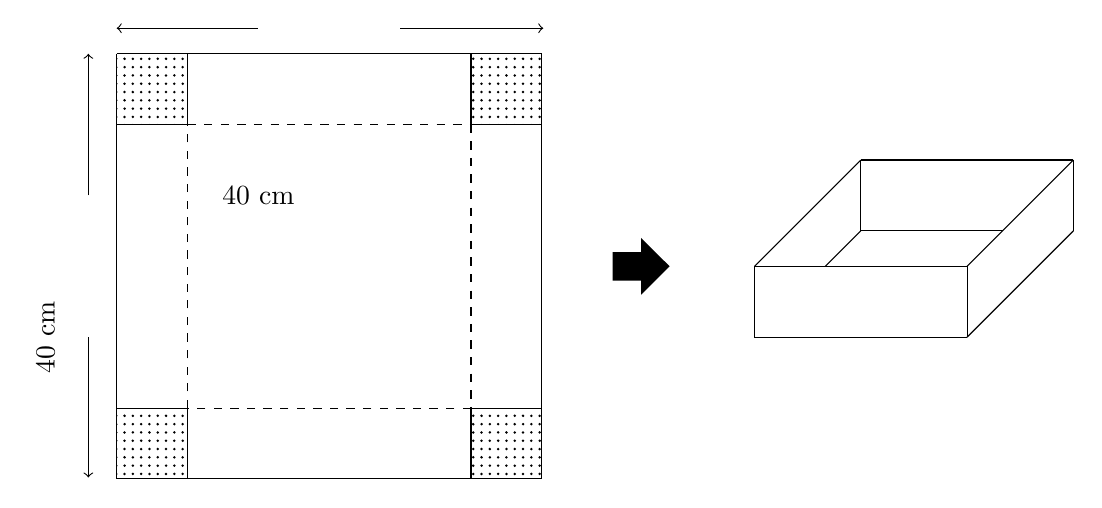
\begin{tikzpicture}[scale=.9]
\usetikzlibrary[patterns]
\fill[fill=black,pattern=dots,pattern color=black] (-3.,3.) -- (-2.,3.) -- (-2.,2.) -- (-3.,2.) -- cycle;
\fill[fill=black,pattern=dots,pattern color=black] (-3.,-2.) -- (-2.,-2.) -- (-2.,-3.) -- (-3.,-3.) -- cycle;
\fill[fill=black,pattern=dots,pattern color=black] (2.,-3.) -- (2.,-2.) -- (3.,-2.) -- (3.,-3.) -- cycle;
\fill[line width=2.pt,fill=black,pattern=dots,pattern color=black] (2.,2.) -- (2.,3.) -- (3.,3.) -- (3.,2.) -- cycle;
\draw [line width=0.4pt, dashed] (-2.,2.)-- (2.,2.);
\draw [line width=0.4pt,dashed] (2.,2.)-- (2.,-2.);
\draw [line width=0.4pt,dashed] (2.,-2.)-- (-2.,-2.);
\draw [line width=0.4pt,dashed] (-2.,-2.)-- (-2.,2.);
\draw [line width=0.4pt] (-3.,2.)-- (-3.,-2.);
\draw [line width=0.4pt] (-2.,-3.)-- (2.,-3.);
\draw [line width=0.4pt] (3.,-2.)-- (3.,2.);
\draw [line width=0.4pt] (2.,3.)-- (-2.,3.);
\draw [line width=0.4pt] (-3.,3.)-- (-2.,3.);
\draw [line width=0.4pt] (-2.,3.)-- (-2.,2.);
\draw [line width=0.4pt] (-2.,2.)-- (-3.,2.);
\draw [line width=0.4pt] (-3.,2.)-- (-3.,3.);
\draw [line width=0.4pt] (-3.,-2.)-- (-2.,-2.);
\draw [line width=0.4pt] (-2.,-2.)-- (-2.,-3.);
\draw [line width=0.4pt] (-2.,-3.)-- (-3.,-3.);
\draw [line width=0.4pt] (-3.,-3.)-- (-3.,-2.);
\draw [line width=0.4pt] (2.,-3.)-- (2.,-2.);
\draw [line width=0.4pt] (2.,-2.)-- (3.,-2.);
\draw [line width=0.4pt] (3.,-2.)-- (3.,-3.);
\draw [line width=0.4pt] (3.,-3.)-- (2.,-3.);
\draw [line width=0.4pt] (2.,2.)-- (2.,3.);
\draw [line width=0.4pt] (2.,3.)-- (3.,3.);
\draw [line width=0.4pt] (3.,3.)-- (3.,2.);
\draw [line width=0.4pt] (3.,2.)-- (2.,2.);
\draw [<-,line width=0.4pt] (-3.4,-2.98) -- (-3.4,-1.);
\draw [->,line width=0.4pt] (-3.4,1) -- (-3.4,3.);
\draw (-4,-1) node[rotate=90] {40 cm};
\draw [<-,line width=0.4pt] (-3.,3.36) -- (-1,3.36);
\draw [->,line width=0.4pt] (1,3.36) -- (3.02,3.36);
\draw (-1,) node {40 cm};
\begin{scope}[xshift=4cm]
\fill[line width=2.pt,fill=black,fill opacity=1.0] (0.,-0.2) -- (0.,0.2) -- (0.4,0.2) -- (0.4,0.4) -- (0.8025630171471898,0.) -- (0.4,-0.4) -- (0.4,-0.2) -- cycle;
\begin{scope}[xshift=2cm, yshift=-1cm]
\draw [line width=.4pt] (0.,0.)-- (0.,1.);
\draw [line width=.4pt] (0.,1.)-- (3.,1.);
\draw [line width=.4pt] (3.,1.)-- (3.,0.);
\draw [line width=.4pt] (3.,0.)-- (0.,0.);
\draw [line width=.4pt] (1.,1.)-- (1.5,1.5);
\draw [line width=.4pt] (3.,0.)-- (4.5,1.5);
\draw [line width=.4pt] (4.5,1.5)-- (4.5,2.5);
\draw [line width=.4pt] (4.5,2.5)-- (1.5,2.5);
\draw [line width=.4pt] (1.5,2.5)-- (1.5,1.5);
\draw [line width=.4pt] (1.5,1.5)-- (3.5,1.5);
\draw [line width=.4pt] (0.,1.)-- (1.5,2.5);
\draw [line width=.4pt] (3.,1.)-- (4.5,2.5);
\end{scope}
\end{scope}
\end{tikzpicture}
\end{figure}
\begin{enumerate}
\item {} 
Discuta com seus colegas de grupo a melhor estratégia para se obter a caixa de volume máximo. Em seguida construa a caixa e calcule o seu volume.

\item {} 
Faça uma comparação com os volumes das caixas construídas pelos demais grupos. Organize os dados em uma tabela que relacione a medida do lado \(x\) do quadrado recortado com o volume \(V(x)\) da caixa obtida.

\begin{figure}[H]
\begin{table}[H]
\centering
\begin{tabu} to \textwidth{|c|c|c|c|c|c|c|c|c|c|c|}
\hline
\cellcolor{\currentcolor!80}{\textcolor{white}{\textbf{x}}} & & & & & & & & & & \\
\hline
\cellcolor{\currentcolor!80}{\textcolor{white}{\textbf{V(x)}}} & & & & & & & & & & \\
\hline
\end{tabu}
\end{table}
\end{figure}

\item {} 
Encontre a expressão que fornece o volume \(V(x)\) da caixa em função do lado \(x\) do quadrado recortado.

\item {} 
No contexto do problema, em que intervalo real a variável independente \(x\) pode ser considerada?

\item {} 
Baseado nos itens anteriores, faça uma conjectura sobre qual o valor de \(x\) fornece o volume máximo.

\item {} 
Utilize um software ou uma calculadora gráfica para visualizar a representação gráfica da função \(V(x)\). A partir dessa representação gráfica determine, aproximadamente, o valor de \(x\) que fornece o volume máximo.

\end{enumerate}
\end{project}

\exercise

\begin{answer}{Exercícios}
{\exerciselist
  \begin{enumerate}
  \item Tempo (variável independente) e altura do nível de água na piscina (variável dependente). A diminuição na altura do nível de água observada nas primeiras 5h deve ser causada pelo vazamento. No período entre 5h e 8h a piscina foi enchida (entrando uma quantidade maior de água do que aquela que está sendo perdida pelo vazamento). A partir das 8h a piscina parou de ser enchida e o vazamento fez com que a altura do nível de água voltasse a diminuir.

  \item
  \begin{enumerate}
  \item $D$
  \item $B$
  \item $A$ e $E$. As garrafas que correspondem a esses pontos são vendidas pelo mesmo preço.
  \item $B$ e $E$. As garrafas que correspondem a esses pontos armazenam a mesma quantidade de água.
  \item $E$ apresenta melhor custo-benefício que $A$, uma vez que ambas são vendidas pelo mesmo preço e $E$ armazena maior quantidade de água. Com relação à $B$, $E$ também apresenta melhor custo-benefício, pois armazena a mesma quantidade de água e custa menos.

  \end{enumerate}
  \end{enumerate}
}{1}
\end{answer}


\label{\detokenize{AF106-E2:sec-exercicios-grafico}}\label{\detokenize{AF106-E2:exercicios}}\label{\detokenize{AF106-E2::doc}}

\begin{enumerate}
\item O gráfico abaixo mostra a altura do nível de água em uma piscina com vazamento. Identifique as variáveis na situação descrita e representada a partir do gráfico. Observe a relação apresentada no gráfico e indique possíveis causas para o comportamento observado.
\begin{center}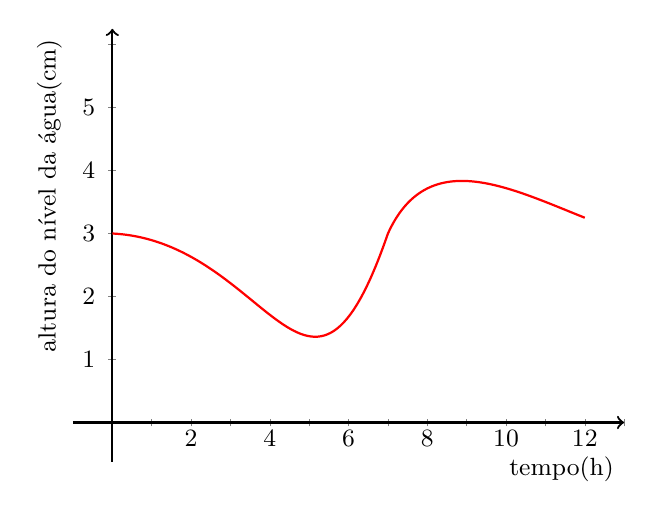
\begin{tikzpicture}
\draw[help lines, gray](0,-.05)grid[xstep=.5](6.5,.05);
\draw[help lines, gray](-.05,0)grid[ystep=.8](.05,5);
\draw[->,  thick](-.5,0)--(6.5,0)node[yshift=-.3cm,below left]{\small tempo(h)};
\draw[->,  thick](0,-0.5)--(0,5)node[left,xshift=-.8cm,rotate=90]{\small altura do nível da água(cm)};
\foreach \x in {2, 4, 6, 8, 10, 12}
\draw(.5*\x,-.2)node{\small \x};
\foreach \x in {1, 2, 3, 4, 5}
\draw(-.3,.8*\x)node{\small \x};
\draw [red,thick,smooth](0,2.4) .. controls (2,2.3)and(2.5,-.5) .. (3.5,2.4)
      (3.5,2.4) .. controls (4,3.5) and (5,3) .. (6,2.6);
\end{tikzpicture}\end{center}

\item Garrafas de água potável são vendidas em vários tamanhos e preços. Cada ponto no gráfico abaixo representa uma garrafa de água.
\begin{center}\begin{tikzpicture}[scale=1.5]
\draw[help lines,xstep=.5cm,ystep=.5cm](0,0)grid(4.7,2.3);
\draw[thick, ->](0,0)--(4.7,0);
\draw[thick, ->](0,0)--(0,2.3);
\draw(3.9,-.2) node {quantidade de \'{a}gua};
\draw(-.15,2) node[rotate=90]{pre\c{c}o};
\draw[fill=\currentcolor!80](1.5,1) circle (1pt) node[above left] {$A$};
\draw[fill=\currentcolor!80](3.5,2) circle (1pt) node[above left] {$B$};
\draw[fill=\currentcolor!80](.5,.5) circle (1pt) node[above left] {$C$};
\draw[fill=\currentcolor!80](4.5,1.5) circle (1pt) node[above left] {$D$};
\draw[fill=\currentcolor!80](3.5,1) circle (1pt) node[above left] {$E$};
\end{tikzpicture}\end{center}\begin{enumerate}
\item {} 
Qual garrafa armazena a maior quantidade de água?

\item {} 
Qual garrafa é vendida pelo preço mais alto?

\item {} 
Identifique dois pontos que estejam sobre uma mesma reta paralela ao eixo das abscissas (reta horizontal) e interprete o que isso significa.

\item {} 
Identifique dois pontos que estejam sobre uma mesma reta paralela ao eixo das ordenadas (reta vertical) e interprete o que isso significa.

\item {} 
Entre as garrafas \(A\) e \(E\), qual tem o melhor custo-benefício? Por que? E entre \(B\) e \(E\)? Por que?

\end{enumerate}
\end{enumerate}


\ifnum\aluno=1
\clearpage
\else
\notasfinais
\fi

\bibliographystyle{apalike-pt}
\bibliography{../Bibliografia/funcoes_bibliografia.bib}

\nocite{*}